% Options for packages loaded elsewhere
\PassOptionsToPackage{unicode}{hyperref}
\PassOptionsToPackage{hyphens}{url}
%
\documentclass[
  12pt,
]{book}
\usepackage{amsmath,amssymb}
\usepackage{lmodern}
\usepackage{iftex}
\ifPDFTeX
  \usepackage[T1]{fontenc}
  \usepackage[utf8]{inputenc}
  \usepackage{textcomp} % provide euro and other symbols
\else % if luatex or xetex
  \usepackage{unicode-math}
  \defaultfontfeatures{Scale=MatchLowercase}
  \defaultfontfeatures[\rmfamily]{Ligatures=TeX,Scale=1}
\fi
% Use upquote if available, for straight quotes in verbatim environments
\IfFileExists{upquote.sty}{\usepackage{upquote}}{}
\IfFileExists{microtype.sty}{% use microtype if available
  \usepackage[]{microtype}
  \UseMicrotypeSet[protrusion]{basicmath} % disable protrusion for tt fonts
}{}
\makeatletter
\@ifundefined{KOMAClassName}{% if non-KOMA class
  \IfFileExists{parskip.sty}{%
    \usepackage{parskip}
  }{% else
    \setlength{\parindent}{0pt}
    \setlength{\parskip}{6pt plus 2pt minus 1pt}}
}{% if KOMA class
  \KOMAoptions{parskip=half}}
\makeatother
\usepackage{xcolor}
\IfFileExists{xurl.sty}{\usepackage{xurl}}{} % add URL line breaks if available
\IfFileExists{bookmark.sty}{\usepackage{bookmark}}{\usepackage{hyperref}}
\hypersetup{
  pdftitle={New User Guide - Drone Use in the UC System},
  pdfauthor={UC Center of Excellence on UAS Safety},
  hidelinks,
  pdfcreator={LaTeX via pandoc}}
\urlstyle{same} % disable monospaced font for URLs
\usepackage{longtable,booktabs,array}
\usepackage{calc} % for calculating minipage widths
% Correct order of tables after \paragraph or \subparagraph
\usepackage{etoolbox}
\makeatletter
\patchcmd\longtable{\par}{\if@noskipsec\mbox{}\fi\par}{}{}
\makeatother
% Allow footnotes in longtable head/foot
\IfFileExists{footnotehyper.sty}{\usepackage{footnotehyper}}{\usepackage{footnote}}
\makesavenoteenv{longtable}
\usepackage{graphicx}
\makeatletter
\def\maxwidth{\ifdim\Gin@nat@width>\linewidth\linewidth\else\Gin@nat@width\fi}
\def\maxheight{\ifdim\Gin@nat@height>\textheight\textheight\else\Gin@nat@height\fi}
\makeatother
% Scale images if necessary, so that they will not overflow the page
% margins by default, and it is still possible to overwrite the defaults
% using explicit options in \includegraphics[width, height, ...]{}
\setkeys{Gin}{width=\maxwidth,height=\maxheight,keepaspectratio}
% Set default figure placement to htbp
\makeatletter
\def\fps@figure{htbp}
\makeatother
\setlength{\emergencystretch}{3em} % prevent overfull lines
\providecommand{\tightlist}{%
  \setlength{\itemsep}{0pt}\setlength{\parskip}{0pt}}
\setcounter{secnumdepth}{5}
\usepackage{booktabs}
\usepackage[margin=1.0in]{geometry}
\usepackage{parskip}
\usepackage{titletoc}
\usepackage[hyphens]{url}
\usepackage{pifont}
\usepackage{amsmath}
\usepackage{amsfonts}
\usepackage{amssymb}

\usepackage{xcolor}
\usepackage{framed}
\setlength{\fboxsep}{.8em}

\newenvironment{notebox}{
  \definecolor{shadecolor}{gray}{.8}  % gray
  \color{black}
  \begin{shaded}}
 {\end{shaded}}
\ifLuaTeX
  \usepackage{selnolig}  % disable illegal ligatures
\fi
\usepackage[]{natbib}
\bibliographystyle{apalike}

\title{New User Guide - Drone Use in the UC System}
\author{UC Center of Excellence on UAS Safety}
\date{}

\begin{document}
\maketitle

{
\setcounter{tocdepth}{1}
\tableofcontents
}
\hypertarget{introduction}{%
\chapter*{Introduction}\label{introduction}}
\addcontentsline{toc}{chapter}{Introduction}

\begin{center}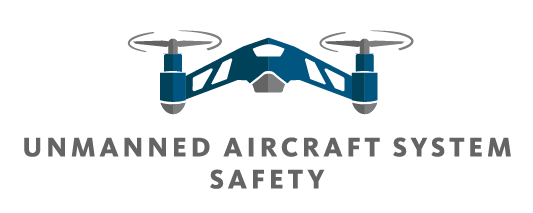
\includegraphics[width=0.5\linewidth]{images/COE_logo} \end{center}

\textbf{The University of California Center of Excellence on Unmanned Aircraft System Safety Presents: New User Guide For Drones}

This guide will walk you through the steps for you start flying for your work or research. This page will be a work in progress and new resources will be added periodically. Feel free to reach out to us at \href{mailto:UASSafety@ucmerced.edu}{\nolinkurl{UASSafety@ucmerced.edu}} if you have any questions or would like to see additional resources added.

Want to schedule an online appointment to chat? Use our \href{https://outlook.office365.com/owa/calendar/UCCenterofExcellenceonUASSafety@merced.onmicrosoft.com/bookings/}{Booking link}. Find a time that works for you and the system will schedule a MS Teams meeting for us.

\textbf{UC Drone Policy}

There is a University of California Drone Policy that governs the use of drones owned by the University of California, the use of drones at any University property, or the use of drones for any University purpose (including teaching, outreach and research). More information about the UC UAS Policy can be found in the UC UAS Policy Guidance Document located at \url{http://UCDrones.github.io/Policy_Guidance/}

\textbf{Policy Requirements}

The Policy establishes that anyone who seeks to operate a UAS under the jurisdiction of the policy must:

\begin{itemize}
\tightlist
\item
  Comply with any applicable regulation, including but not limited to any applicable FAA regulation.
\item
  Have prior approval from the Campus Drone Person or the Systemwide Designated Authority.
\item
  Operate in a manner that ensures public safety, right to privacy, civil rights and civil liberties.
\item
  Maintain sufficient liability insurance coverage.
\end{itemize}

The UC Center of Excellence on UAS Safety is here to help you guide you through the process.

\textbf{Step-by-step UC Drone Process}

\begin{enumerate}
\def\labelenumi{\arabic{enumi}.}
\tightlist
\item
  Register your drone with the \protect\hyperlink{registration}{FAA} and UC
\item
  Get an \protect\hyperlink{license}{FAA Drone License} (or figure out if you're \protect\hyperlink{difference}{exempt}) and register yourself with the UC
\item
  Find a place to fly - review \protect\hyperlink{airspace-info}{airspace}, \protect\hyperlink{safety-guidelines}{safety guidelines} and \protect\hyperlink{local-regulations}{local regulations}
\item
  Submit a \protect\hyperlink{UCDrones-project}{UC Flight Request}
\item
  Fly Safely
\item
  Submit a Post-Flight Report
\end{enumerate}

\textbf{Click the Next Arrow, or Choose a Chapter to Begin}

\hypertarget{regulations}{%
\chapter{Drone Rules and Regulations}\label{regulations}}

Welcome to the world of Drones! We're always happy to see new drone pilots and new drone projects. But first, we have to introduce you to the ever-changing drone regulations.

\begin{notebox}
Don't forget that following the \textbf{DRONE} regulations are only one part of the UC Drone Policy. Local rules, environmental regulations, export control, and even insurance requirements may require additional steps or have additional restrictions. Helping you navigate through all of this is part of the UC Drone Flight Request process.

\end{notebox}

\textbf{The Main 7 Rules}

\begin{enumerate}
\def\labelenumi{\arabic{enumi}.}
\tightlist
\item
  Don't do anything unsafe
\item
  All drones must be registered
\item
  All pilots must have either a Drone License or a TRUST certificate
\item
  No flying farther than you can see
\item
  No flying over people
\item
  No flying above 400 ft
\item
  Stay away from other aircraft
\end{enumerate}

There's a lot of details behind the above rules, including several exceptions. So let's dive into them in more detail.

\hypertarget{basic-drone-rules}{%
\section{Basic Drone Rules}\label{basic-drone-rules}}

In this page, we'll introduce some of the basic drone rules. Basically, the rules for operating a drone can be boiled down to \textbf{``Do not do anything unsafe''} - but sometimes they have to be spelled out.

\hypertarget{drone-operating-rules}{%
\subsection{Drone Operating Rules}\label{drone-operating-rules}}

\begin{itemize}
\tightlist
\item
  No flying farther than you can clearly see the drone

  \begin{itemize}
  \tightlist
  \item
    You must be able to see the drone at all times
  \end{itemize}
\end{itemize}

\begin{figure}

{\centering 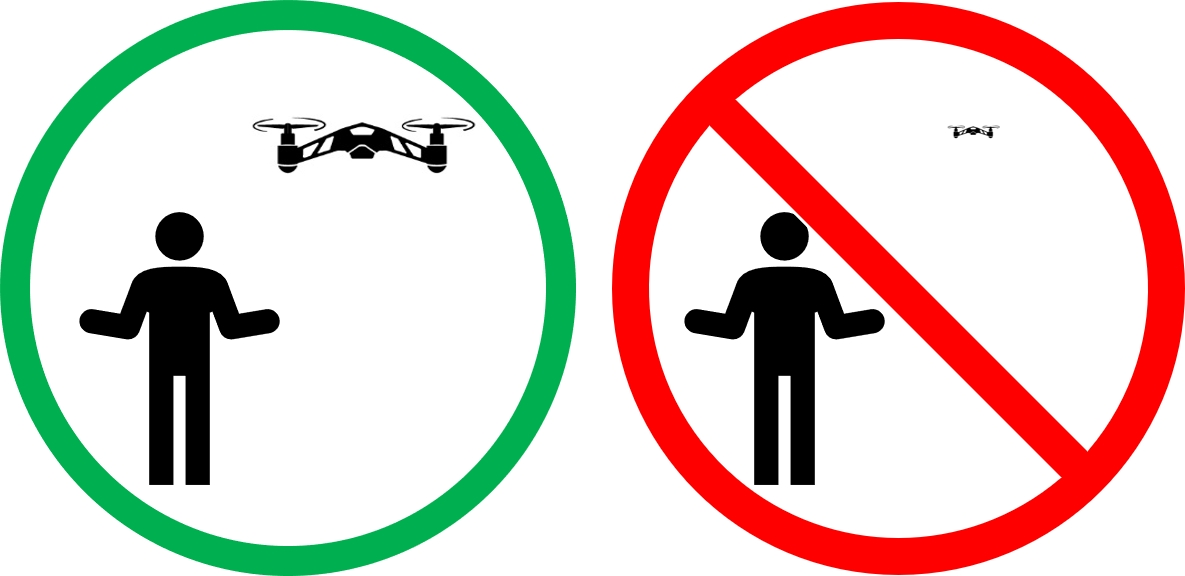
\includegraphics[width=0.7\linewidth]{images/VLOS_simple} 

}

\caption{Visual Line of Sight}\label{fig:VLOS}
\end{figure}

\begin{itemize}
\tightlist
\item
  No flying above non-participants or moving cars
\item
  No flying higher than 400 ft above the ground
\item
  No reckless or careless flying that endangers the life or property of another
\item
  No flying when the horizon visibility drops below 3 miles

  \begin{itemize}
  \tightlist
  \item
    This includes smog, fog, or haze
  \end{itemize}
\item
  No flying within 2000 ft laterally or 500 ft vertically of any cloud

  \begin{itemize}
  \tightlist
  \item
    Including fog and low cloud layers on overcast days
  \end{itemize}
\end{itemize}

\begin{figure}

{\centering 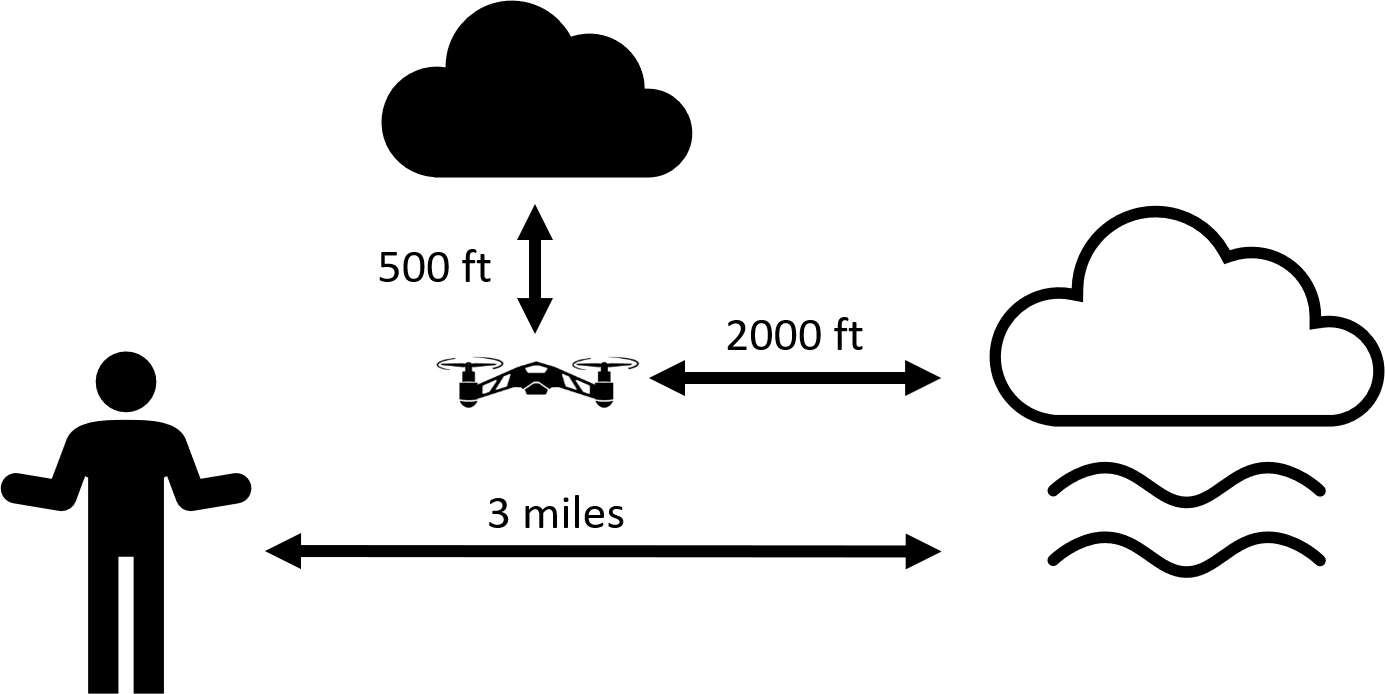
\includegraphics[width=0.7\linewidth]{images/cloud_distance} 

}

\caption{Minimum Distances from Clouds, Fog or Haze}\label{fig:cloud-distance}
\end{figure}

\begin{itemize}
\tightlist
\item
  No flying faster than 100 mph
\item
  No flying at night
\item
  No operating a drone from a moving vehicle
\end{itemize}

\hypertarget{airspace-rules}{%
\subsection{Airspace Rules}\label{airspace-rules}}

\begin{itemize}
\tightlist
\item
  The drone must always get out of the way and always stay well-clear of all manned aviation traffic, including airplanes, helicopters, gliders, paragliders, hot air balloons and parachutes.

  \begin{itemize}
  \tightlist
  \item
    Even if ``you were there first''
  \end{itemize}
\item
  Permission is required to fly in any controlled airspace (Class B, C, D, and surface Class E)

  \begin{itemize}
  \tightlist
  \item
    Controlled airspace is typically found within 5 miles of most airports for commercial travel and large general aviation airports (non-commercial travel) - See Figure \ref{fig:SUAS-airspace-regs}
  \end{itemize}
\end{itemize}

\begin{figure}

{\centering 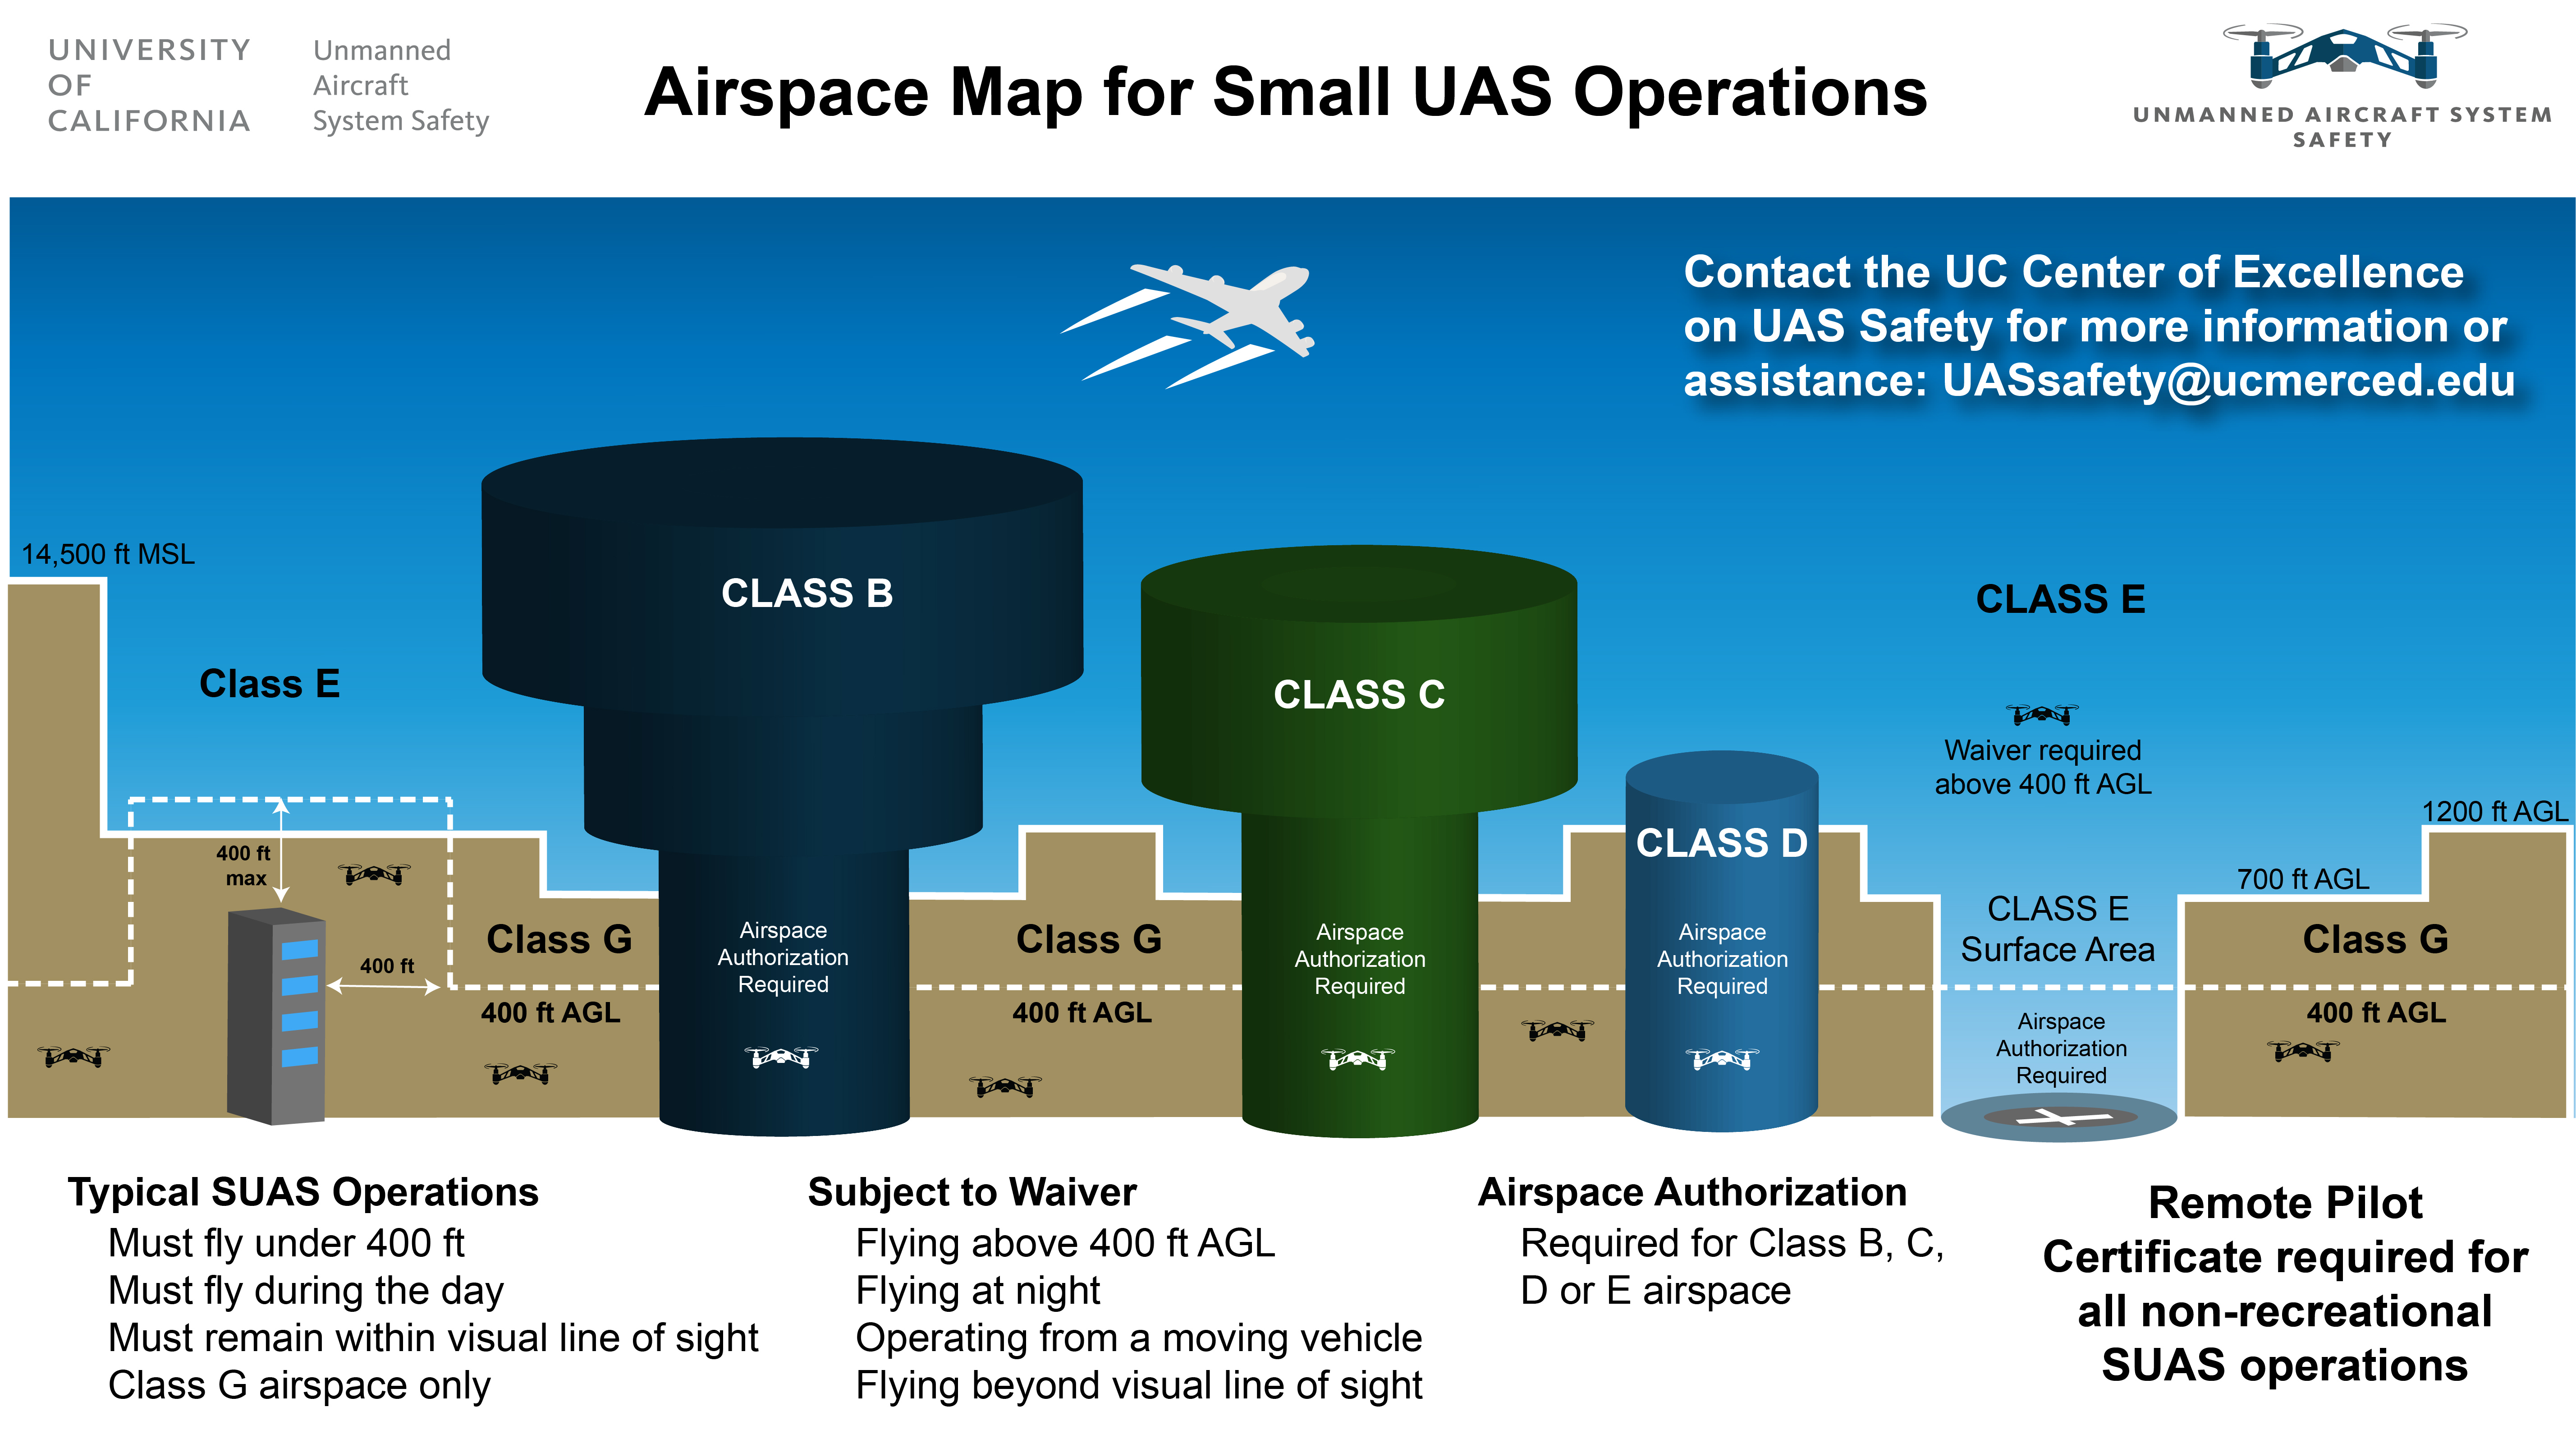
\includegraphics[width=0.9\linewidth]{images/SUAS_airspace_map} 

}

\caption{Small UAS Airspace Rules}\label{fig:SUAS-airspace-regs}
\end{figure}

\begin{itemize}
\tightlist
\item
  No interfering with aviation traffic patterns at any airport, heliport, or seaplane base

  \begin{itemize}
  \tightlist
  \item
    Traffic patterns include more than just the immediate take off and landing - it also includes the downwind and base legs (See Figure \ref{fig:traffic-patterns})
  \end{itemize}
\end{itemize}

\begin{figure}

{\centering 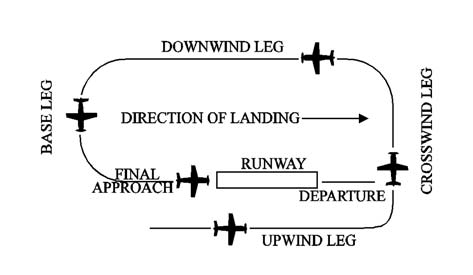
\includegraphics[width=0.6\linewidth]{images/faa_traffic_pattern} 

}

\caption{Typical Airport Traffic Patterns (FAA Aeronautical Information Manual)}\label{fig:traffic-patterns}
\end{figure}

\hypertarget{operator-rules}{%
\subsection{Operator Rules}\label{operator-rules}}

\begin{itemize}
\tightlist
\item
  There must always be a Remote Pilot in Command (RPIC)

  \begin{itemize}
  \tightlist
  \item
    The RPIC is the one in charge of the flight operations and is ultimately responsible for all safety and operations
  \item
    The RPIC doesn't always have to be the one manipulating the flight controls of the drone - it could be the RPIC is letting a student learn to fly under his/her direct supervision.
  \item
    The RPIC may only operate (supervise) one drone at a time
  \end{itemize}
\item
  The RPIC must have an FAA Drone License (or be exempt*)

  \begin{itemize}
  \tightlist
  \item
    More Info Here: \protect\hyperlink{ch-license}{FAA Drone License}
  \end{itemize}
\item
  The RPIC must be at least 16 years of age, and must be able to speak, write and understand English.

  \begin{itemize}
  \tightlist
  \item
    No restriction on nationality but a license does require Federal documentation such as a Passport.
  \end{itemize}
\item
  No one may operate a drone or act as any direct participant in the operation of a drone if he or she knows, or has reason to know, that he or she has a physical or mental condition that would interfere with the safe operation of the drone.
\item
  No one may operate a drone or act as any direct participant in the operation of a drone under the influence of alcohol or any drug that may inhibit decision making
\end{itemize}

\begin{figure}

{\centering 
\includegraphics[width=0.7\linewidth]{images/no_drugs} 

}

\caption{No drugs, alcohol or altered mind-states allowed during flight operations}\label{fig:drugs}
\end{figure}

\hypertarget{drone-rules}{%
\subsection{Drone Rules}\label{drone-rules}}

\begin{itemize}
\tightlist
\item
  All drones that weigh more than 0.55 lbs (250 grams) must be registered with the FAA

  \begin{itemize}
  \tightlist
  \item
    Only use the FAA DroneZone website for registration (More Info here: \protect\hyperlink{ch-registration}{Register your Drone})
  \end{itemize}
\end{itemize}

\begin{figure}

{\centering 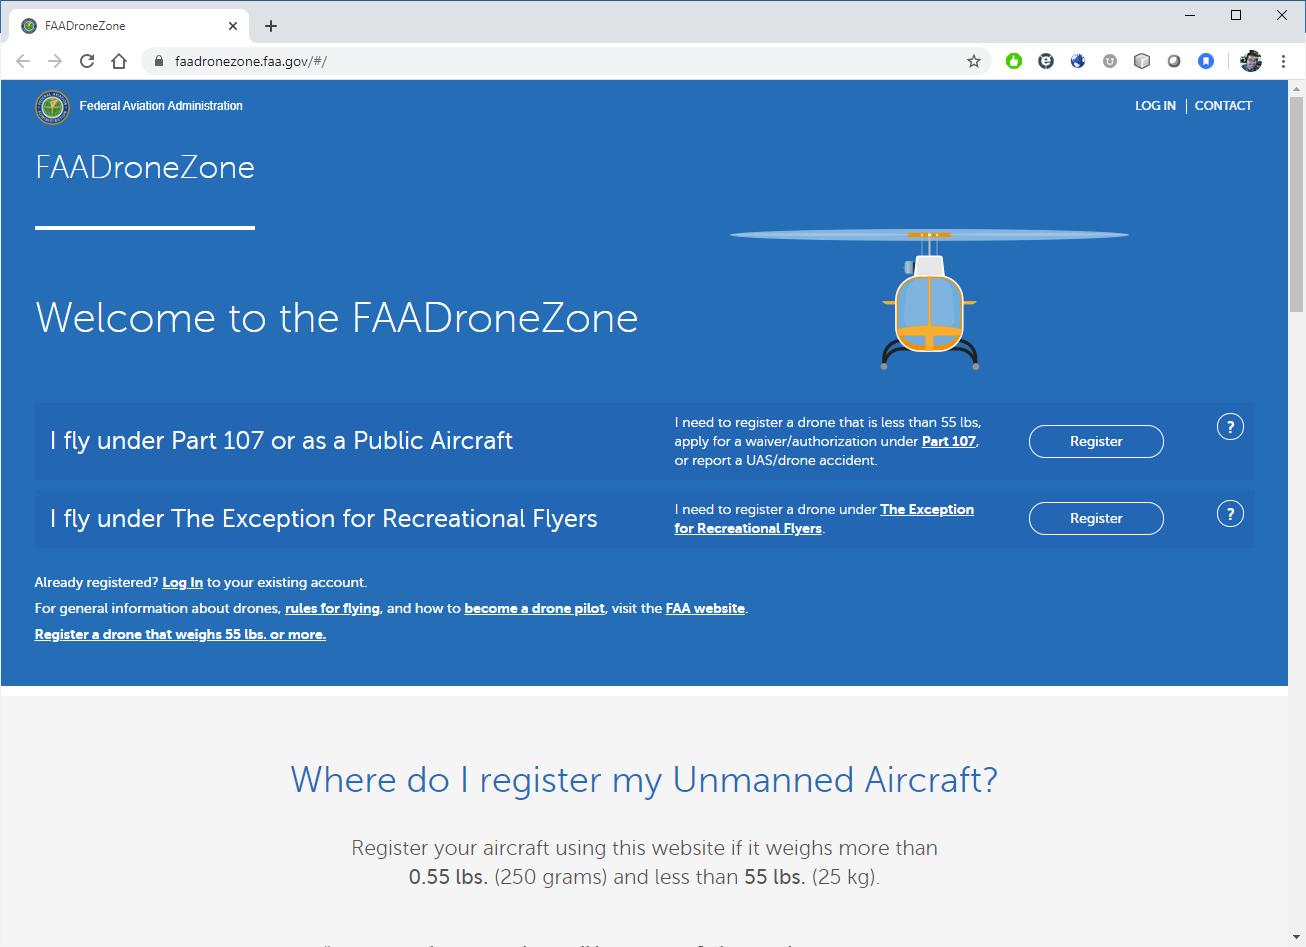
\includegraphics[width=0.8\linewidth]{images/reg_site} 

}

\caption{FAA DroneZone}\label{fig:reg-page2}
\end{figure}

\begin{itemize}
\tightlist
\item
  Drones must weigh less than 55 lbs

  \begin{itemize}
  \tightlist
  \item
    Drones that weigh more than 55 lbs require rare special FAA authorization
  \end{itemize}
\item
  Drones may not drop or release hazardous material

  \begin{itemize}
  \tightlist
  \item
    Drones that drop biological or chemical agents for Agriculture require additional Federal and State authorizations
  \item
    While not illegal, please do not drop glitter or confetti from a drone
  \end{itemize}
\item
  Any payload that is attached to the drone must be securely attached and may not adversely affect the controllability of the drone
\item
  Weapons are not allowed to be attached or used on drones
\item
  Tethered drones are not exempt from drone regulations
\end{itemize}

\begin{notebox}
The topic of drone regulations can be very nuanced and complex. We've shortened it to the basics in this section, but there may be scenarios or situations that may be exempt or have additional restrictions. Always feel free to reach out to us at \href{mailto:UASsafety@ucmerced.edu}{\nolinkurl{UASsafety@ucmerced.edu}} for a one-on-one consultation.

\end{notebox}

\hypertarget{registration}{%
\section{Drone Registration}\label{registration}}

\begin{notebox}
This page is for the registration of your drone with the Federal Aviation Administration. For information on how to register your drone with the UC system, see Chapter \ref{UCDrones-drone}.

\end{notebox}

\hypertarget{drone-registration-requirements}{%
\subsection{Drone Registration Requirements}\label{drone-registration-requirements}}

All drones that weigh more than 0.55 lbs (250 grams) must be registered with the Federal Aviation Administration (FAA) to it's legal owner.

Any drone purchased through the University of California for university business, including teaching and research, is owned by the \textbf{Regents of the University of California}.

\hypertarget{how-to-register}{%
\subsection{How to Register}\label{how-to-register}}

You can register the drone through the FAA Drone Zone (\url{https://faadronezone.faa.gov}). Registration costs only \$5 per aircraft and only takes a couple of minutes.

\hypertarget{create-an-account-at-dronezone}{%
\subsection{Create an account at DroneZone}\label{create-an-account-at-dronezone}}

Head to the FAA DroneZone (\url{https://faadronezone.faa.gov}) and select ``I fly under Part 107 or as a Public Aircraft'' \ref{fig:reg-page}

\begin{figure}

{\centering 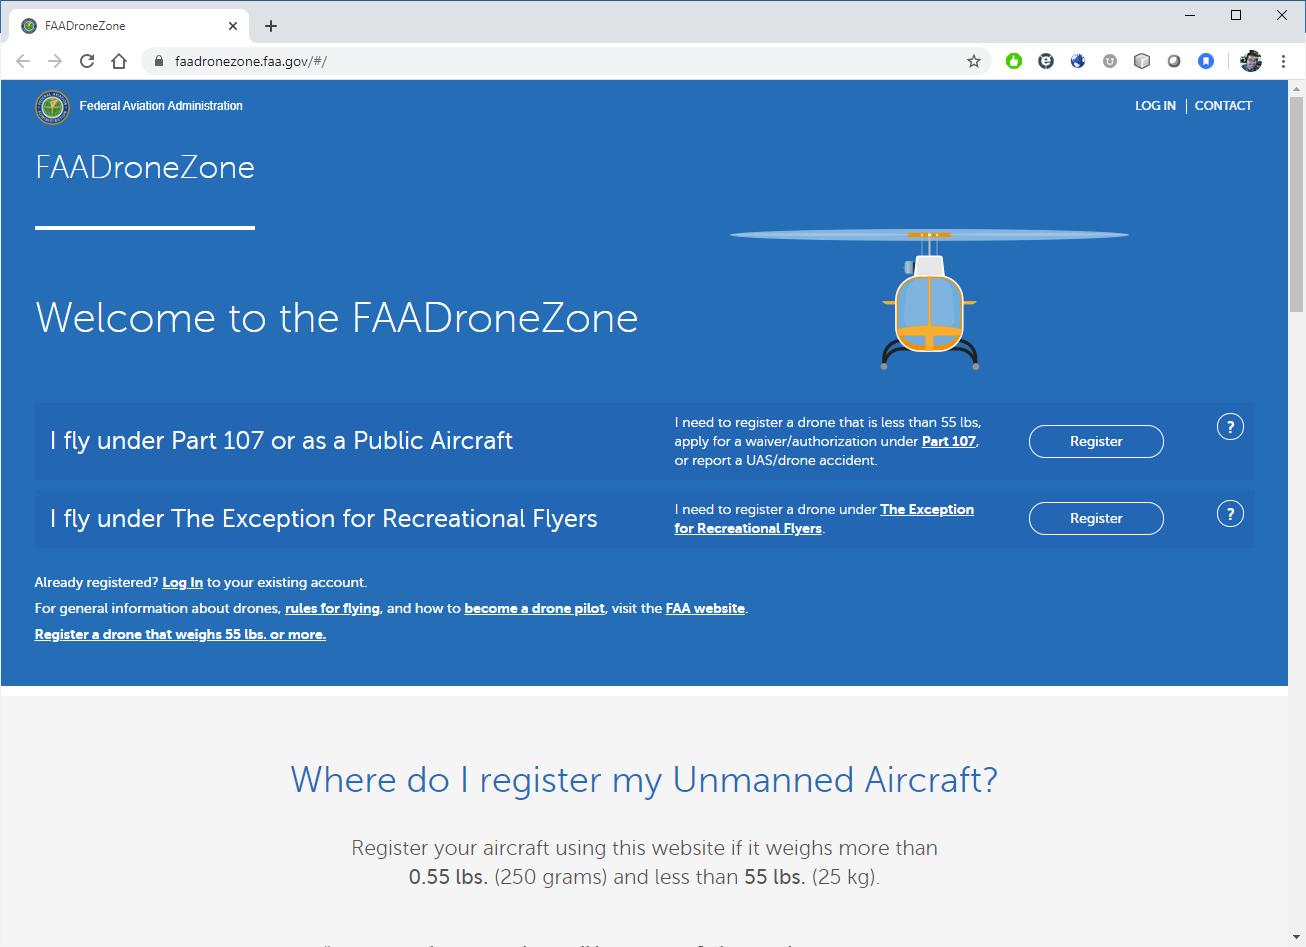
\includegraphics[width=0.8\linewidth]{images/reg_site} 

}

\caption{FAA DroneZone}\label{fig:reg-page}
\end{figure}

\textbf{Important Note} Unfortunately, the FAA's drone registration website does not allow you to register drones for multiple groups or organizations. If you're registering a drone on behalf of the University of California, you should use your UC email address as your account log in, and use a personal email address account for any personally-owned drones.

When you enter your Part 107 Account information, enter \textbf{Regents of the University of California} as your Part 107 Account Name to correctly register the drone to the UC system.

\begin{notebox}
If you already have an account, go into your profile settings, and you can modify the \textbf{Part 107 Account Name} on the popup.

\end{notebox}

\hypertarget{drone-registration}{%
\subsection{Drone Registration}\label{drone-registration}}

Once you have an account, on the dashboard will be an option to `Manage sUAS Inventory.' On that page, you'll be able to `Add UAS' (in the upper right corner). This will bring up a dialog box (Figure \ref{fig:add-UAS}) for you to enter your information. Enter all the relevant information.

\begin{figure}

{\centering 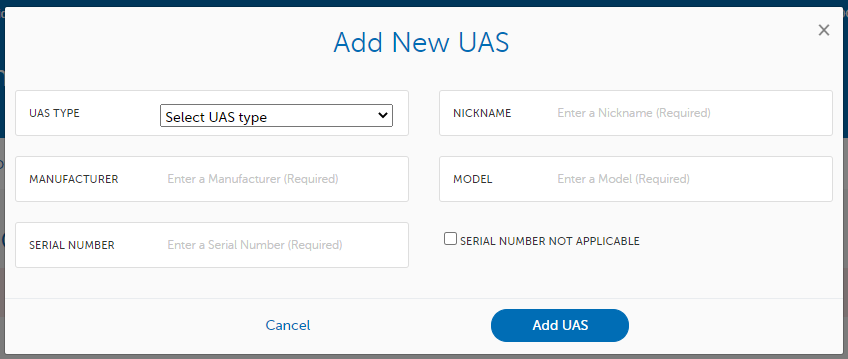
\includegraphics[width=0.8\linewidth]{images/Add_new_UAS} 

}

\caption{Add new UAS Dialog Box}\label{fig:add-UAS}
\end{figure}

Once completed, `Your Shopping Cart' will now show this drone's information and a new buttom for `Checkout' will appear. Click the button and the system will guide you through paying for the registration fee.

\hypertarget{registration-certificate}{%
\subsection{Registration Certificate}\label{registration-certificate}}

Upon completion of paying for registration, the DroneZone will send you two emails, one with a receipt of payment and the other is a pdf copy of your UAS registration certificate (Figure \ref{fig:reg-cert}). Keep a copy of this registration certificate available at all times while you operate. This can be done by either printing it out and placing it with your drone, or keeping a digital copy on your phone.

\begin{figure}

{\centering 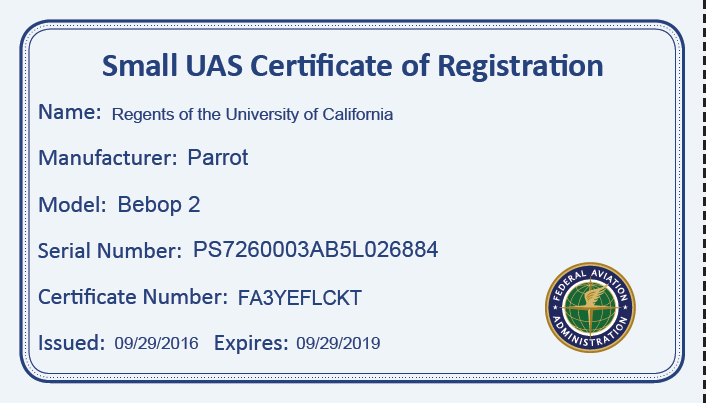
\includegraphics[width=0.5\linewidth]{images/reg_cert} 

}

\caption{Example UAS Registration Certificate}\label{fig:reg-cert}
\end{figure}

\hypertarget{marking-the-drone}{%
\subsection{Marking the Drone}\label{marking-the-drone}}

Your drone's registration number is the 10 digit alphanumeric code that starts with \textbf{FA}. You must mark this on your drone on an external location, where it can be plainly visible.

We recommend either using a permanent oil-based fine tip paint marker (Figure \ref{fig:markers}) or creating a label that can be strongly affixed to the drone. We've found that regular sharpies or markers are rubbed off too easily to be effective.

\begin{figure}

{\centering 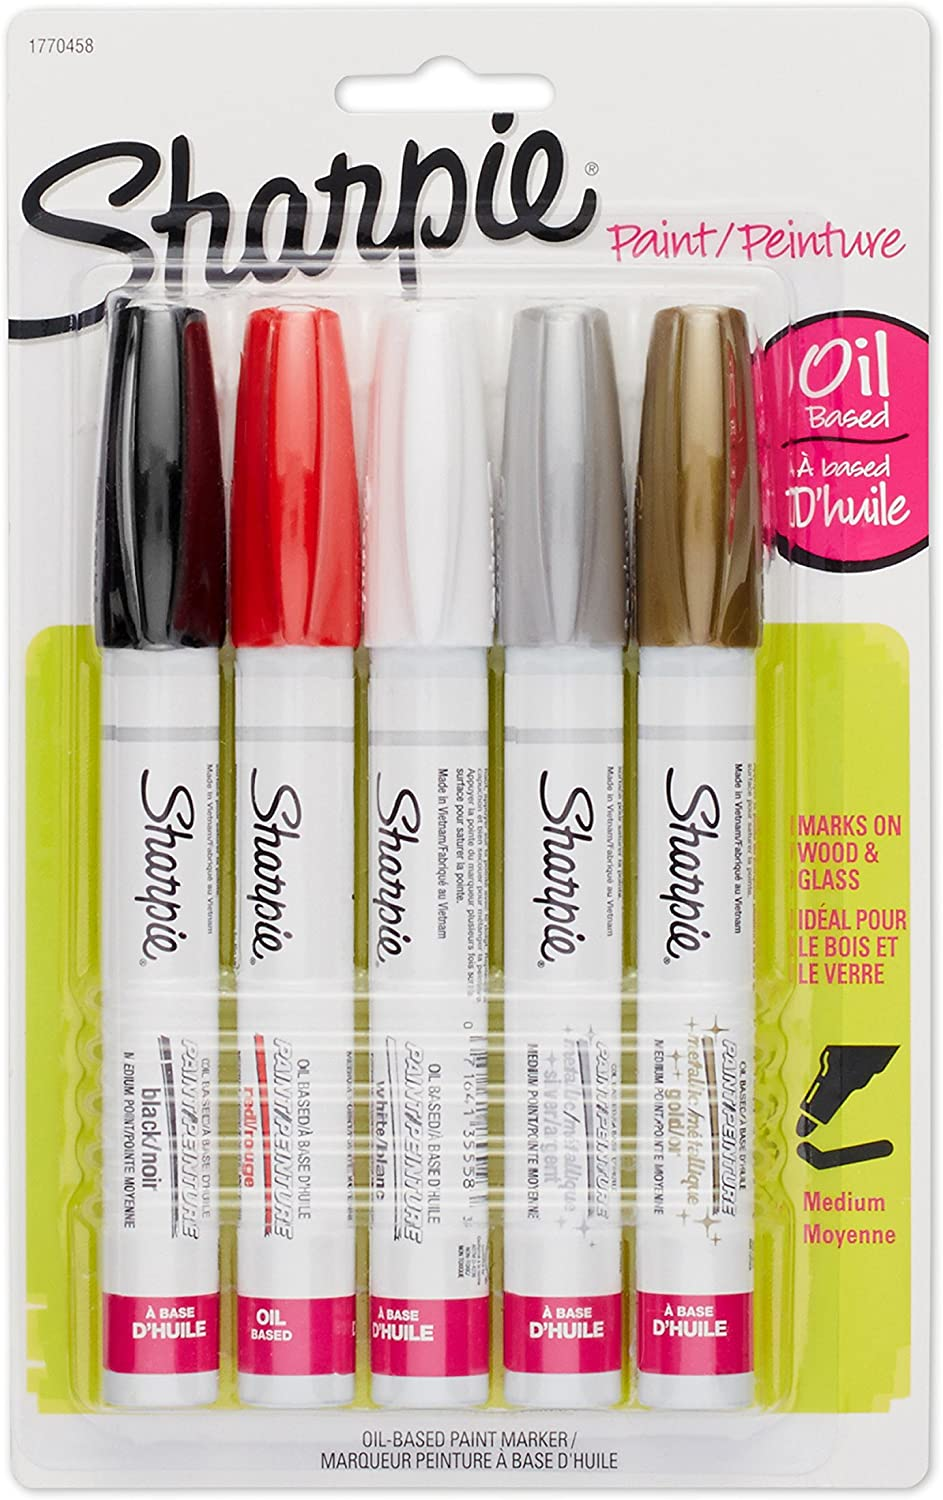
\includegraphics[width=0.5\linewidth]{images/oil-based-markers} 

}

\caption{Oil-Based Paint Markers}\label{fig:markers}
\end{figure}

If you'll be working with a fleet of aircraft, it may also be useful to mark the `nickname' of the drone as well.

\hypertarget{license}{%
\chapter{FAA License Information}\label{license}}

When operating a drone within the US, there are \textbf{two} different options for regulations: \textbf{Part 107 Small UAS regulations} or the \textbf{Exception for Limited Recreational Use}. By default, UAS operations fall under Part 107 Small UAS regulations, unless you can meet the requirements for the exception for Recreational Use. Part 107 requires that all pilots have a \textbf{Remote Pilot Certificate with an sUAS rating}, more commonly known as a `Drone License,' whereas Recreational Use requires a \textbf{TRUST certificate}.

As of June 2021, \textbf{all drone pilots} must have either:

\begin{enumerate}
\def\labelenumi{\arabic{enumi}.}
\tightlist
\item
  \protect\hyperlink{get-license}{Remote Pilot Certificate (Drone License)}
\item
  \protect\hyperlink{TRUST}{TRUST Certificate}
\end{enumerate}

Many researchers opt to get a \protect\hyperlink{get-license}{Drone License} for their research needs, but a Drone License does cost \$150 and will take some time to study and prepare for. With the updates introduced in the FAA Reauthorization Act of 2018 (P.L. 115-254), there are more exceptions available in which you may not need to obtain the license.

The \protect\hyperlink{TRUST}{Recreational UAS Safety Test (TRUST) certificate} is a new requirement for all drone pilots without a Drone License. The TRUST certificate is free for everyone, can be done online and takes 20-30 minutes to complete the training. You can obtain your TRUST certificate by completing the drone training at any of websites listed on the FAA's website here: \url{https://www.faa.gov/uas/recreational_fliers/knowledge_test_updates/}

\begin{notebox}
This page is for the Federal Aviation Administration licensing requirements for UAS use. UC Policy will still require a flight request and post flight reporting, regardless of FAA licensing requirements. More information on submitting flight requests can be found in Chapter \ref{UCdrones}.

\end{notebox}

\hypertarget{difference}{%
\section{Which should I Get?}\label{difference}}

The Part 107 Remote Pilot Certificate, or Drone License, provides for the widest range of permissions and allowances. But there are many cases where a researcher may be satisfied with operating only under the Recreational Exception.

But let's explain the difference between the two.

\textbf{Under Part 107}

\begin{itemize}
\tightlist
\item
  Drone License required
\item
  May fly for any purpose
\item
  `Fly only when it is safe'

  \begin{itemize}
  \tightlist
  \item
    The pilot is responsible for determining whether the environment and all conditions are safe for a drone flight. The pilot must their best judgment to assess whether the proposed flight operation will put anyone at risk.
  \end{itemize}
\item
  May request special permissions

  \begin{itemize}
  \tightlist
  \item
    Above FAA Facility Map altitudes
  \item
    Over People, BVLOS, More than 1 drone at a time
  \end{itemize}
\end{itemize}

\textbf{Under Recreational Exception}

\begin{itemize}
\tightlist
\item
  TRUST certificate required
\item
  May fly only for \textbf{Recreation or Approved Academic Activities}
\item
  `Fly only in safe locations'

  \begin{itemize}
  \tightlist
  \item
    The site has been designated by an organization, or is sufficiently clear and controlled, that this environment and location poses the least amount of risk to all participants. The pilot is still responsible for ensuring the safety of the flight, but the location is generally expected to be completely safe.
  \end{itemize}
\item
  No allowances for advanced operations

  \begin{itemize}
  \tightlist
  \item
    Must stick to the \textbf{basic rules} for flight operations
  \end{itemize}
\end{itemize}

Flight operations in \textbf{access controlled locations}, such as UC Reserves or agricultural field stations, are generally acceptable for the Recreational Exception. The use of a \textbf{reserved campus field}, such as an Intramural Athletic Field or a Campus quad, may also be acceptable for the Recreational Exception as well.

\hypertarget{approved-academic-activities}{%
\subsection{Approved Academic Activities}\label{approved-academic-activities}}

You may not need a drone license if your flight operations can fit under the stipulations listed for `recreational' activities \textbf{and} your flight operations are related to

\begin{itemize}
\tightlist
\item
  Coursework
\item
  Instruction of students
\item
  Academic or research related uses of unmanned aircraft systems that have been approved by the institution
\item
  Activities undertaken by the institution as part of research projects
\item
  Other academic activities approved by the institution
\end{itemize}

Note that there is no restriction on \textbf{who} the approved academic activities can apply to. \textbf{Any person associated with the University undertaking the above academic activities are eligible}, this includes academic staff or academic support staff. For example, a staff member at a UC Reserve may operate under the academic exception when conducting research activities.

\begin{notebox}
However, not all UC activity is academic, even if it is for an academic group. For example, a student flying a drone to take pictures of the Engineering Hall for the Engineering Department is not considered academic.

\end{notebox}

\hypertarget{simple-drone-regulations}{%
\subsection{Simple Drone Regulations}\label{simple-drone-regulations}}

Recreational flight operations, despite what you see on YouTube, have strict requirements:

\begin{itemize}
\tightlist
\item
  Only fly below 400 ft
\item
  Must stay within Visual Line of Sight
\item
  Must fly only in safe areas and no closer than 25 ft to any individuals
\item
  Must use an established safety line to separate all operations from spectators and bystanders
\item
  Must get FAA authorization to fly in Controlled Airspace (Class B, Class C, Class D and surface Class E)
\item
  Never fly over any person or moving vehicle
\item
  Never interfere with any manned aircraft or emergency response activity
\item
  Never fly under the influence of drugs or alcohol
\item
  Never operate in a careless or reckless manner
\end{itemize}

In many cases, these regulations are not that restrictive. For research activities in a controlled location, such as an agricultural field station or a natural reserve, it is often easy to abide by these regulations.

\begin{notebox}
Commonly the restriction that moves an activity into requiring a Drone license is the proximity to people and buildings, or the activity does not meet the definition of an academic activity. Some example scenarios are discussed in the Frequently Asked Question section in Chapter \ref{license-FAQ}.

\end{notebox}

\hypertarget{other-situations}{%
\subsection{Other Situations}\label{other-situations}}

There are other conditions that may require a closer evaluation, including whether you're a US citizen or if you plan on flying internationally. If you have any questions, feel free to reach out to \href{mailto:UASsafety@ucmerced.edu}{\nolinkurl{UASsafety@ucmerced.edu}} for a consultation.

Other scenarios that may require a closer look

\begin{itemize}
\tightlist
\item
  Performing a demonstration
\item
  Not a US citizen
\item
  Flying above 400 ft AGL
\item
  Flying in fog or with limited visibility
\item
  Flying at night
\item
  Flying internationally
\end{itemize}

Once you know which authorization you need, continue on to read more about how to get it.

\begin{enumerate}
\def\labelenumi{\arabic{enumi}.}
\tightlist
\item
  \protect\hyperlink{get-license}{Remote Pilot Certificate (Drone License)}
\item
  \protect\hyperlink{TRUST}{TRUST Certificate}
\end{enumerate}

\hypertarget{get-license}{%
\section{Drone License}\label{get-license}}

Obtaining a Remote Pilot Certificate, or more commmonly known as a drone license, is relatively straight-forward. The process is similar to obtaining a drivers license, but with one key exception: there is no `driving' test component. To get a drone license, you must study for and pass a drone license exam that tests only on your knowledge of aviation rules and safety.

\begin{notebox}
The FAA has found that on average, most people study for the exam for about 20 hours and that 90\% of test takers pass on the first try. The exam is not particularly challenging, but it requires a lot of memorization.

\end{notebox}

\hypertarget{drone-license-exam}{%
\subsection{Drone License Exam}\label{drone-license-exam}}

The drone license exam (airman knowledge test) is a 120 minute, 60 question exam that goes over a wide range of topics. The topics covered on the exam can be broken down into 12 sections as follows:

\begin{enumerate}
\def\labelenumi{\arabic{enumi}.}
\tightlist
\item
  General UAS regulations
\item
  Airspace classifications
\item
  Aviation weather sources
\item
  Loading and Performance
\item
  Emergency procedures
\item
  Crew resource management
\item
  Radio communication procedures
\item
  Determining UAS performance
\item
  Physiological effects of drugs and alcohol
\item
  Aeronautical decision-making and judgment
\item
  Airport operations
  and
\item
  Maintenance and pre-flight inspection procedures.
\end{enumerate}

A more in depth look at these topics can be found on the FAA's website here: (\url{https://www.faa.gov/regulations_policies/handbooks_manuals/aviation/media/remote_pilot_study_guide.pdf})

The most important and most difficult part of the exam is learning how to read and understand the Airspace Maps. Airspace maps pack a lot of information in a small space, so they often look very overwhelming and complex. For more information on how read Airspace Maps, check our tutorial here: Reading an Airspace Map.

\hypertarget{free-study-resources}{%
\subsection{Free study resources}\label{free-study-resources}}

Here are a few free study resources to aid in studying for the exam:

\begin{itemize}
\tightlist
\item
  (\url{https://jrupprechtlaw.com/part-107-test-study-guide})
\item
  (\url{https://northrup.photo/free-faa-part-107-suas-drone-certification-study-guide/})
\item
  (\url{https://www.3dr.com/docs/faa-part-107-study-guide/part-107-certification-official-study-resources/})
\end{itemize}

\begin{notebox}
Although there are third party ``Ground school'' courses offered for a fee, we have found freely available resources to be just as effective.

\end{notebox}

\hypertarget{drone-license-eligibility}{%
\subsection{Drone License Eligibility}\label{drone-license-eligibility}}

In order to be eligible to obtain a Remote Pilot Certificate, you must meet the following requirements:

\begin{itemize}
\tightlist
\item
  Be at least 16 years of age
\item
  Be able to read, speak and understand the English language. If the applicant is unable to meet one of these requirements due to medical reasons, the FAA may place such operation limitations on that applicant's certificate as are necessary for the safe operation of the small unmanned aircraft.
\item
  Not know or have reason to know that he or she has a physical or mental condition that would interfere with the safe operation of a small unmanned aircraft system.
\end{itemize}

However, to take the FAA Airman Knowledge Exam, the proponent must prove their identity with a valid photo ID that includes their date of birth, signature and physical, residential address.

For U.S. Citizens and U.S. Resident Aliens, this may be accomplished with one of the following:

\begin{itemize}
\tightlist
\item
  Driver Permit or License issued by a U.S. state or territory
\item
  U.S. Government Identification Card
\item
  U.S. Military Identification Card
\item
  Passport
\item
  Alien Residency Card
\end{itemize}

For Non-U.S. Citizens, this may be accomplished with one of the following:

\begin{itemize}
\tightlist
\item
  Passport and a Driver permit or license issued by a U.S. state or territory.
\item
  Passport and an Identification card issued by any governmental entity.
\end{itemize}

\hypertarget{taking-the-drone-exam}{%
\subsection{Taking the Drone Exam}\label{taking-the-drone-exam}}

The process to take the drone exam is a bit more complicated than just signing up for it. This is a short overview of the process - for more details, you can visit the FAA's website here: \href{https://www.faa.gov/uas/commercial_operators/become_a_drone_pilot/}{Becoming a Drone Pilot}

\begin{enumerate}
\def\labelenumi{\arabic{enumi}.}
\item
  Obtain an \textbf{FAA Tracking Number (FTN)} by creating an \textbf{Integrated Airman Certification and Rating Application (IACRA)} profile prior to registering for a knowledge test. Go to \url{https://iacra.faa.gov/IACRA/Default.aspx} to create your profile. Make sure you write down your FTN because you'll need it to register for the drone test in the next step.
\item
  Schedule an appointment with a FAA-approved Knowledge Testing Center. We recommend using the \href{https://faa.psiexams.com/faa/login}{PSI Exams website} to search for a nearby FAA testing facility and registering for the exam. The test you are looking for is \textbf{Unmanned Aircraft General -- Small (UAG)}.
\item
  Study and do a good job on the test. Be sure to bring a government-issued photo ID to your test.
\item
  After you complete the test, you'll need to go back to the \textbf{IACRA} system to register your score. Don't worry, your testing center will provide you with the instructions on how to do this.
\end{enumerate}

Once you register your score with the FAA, they will send you your permanent remote pilot certificate via mail. This might take 4-6 weeks to process, but in the interim, you can download a temporary permit from the IACRA website.

\hypertarget{license-renewal}{%
\subsection{License Renewal}\label{license-renewal}}

In order to maintain your authorization to fly a drone using your Remote Pilot Certificate, you need to renew it every two years. Starting in April 2021, the recurrent knowledge training is now available for free and online.

\textbf{Part 107 Small UAS Recurrent Non-Part 61 Pilots (ALC-677)}

Available at: \url{https://www.faasafety.gov/gslac/ALC/course_content.aspx?cID=677}.

\hypertarget{training-information}{%
\subsubsection{Training Information}\label{training-information}}

The training consists of 3 modules - Introduction, Aircraft and RPIC Requirements, and Safe Operation of sUAS. Each module will have some knowledge tests inside, and after completion of all three modules, there is the required online end-of-training knowledge check. And it has the new information about remote ID, flying over people and flying at night operations. The end-of-training knowledge check is a 45 question test -- you'll have 90 minutes to complete it, and while you can't leave the page, you're welcome to open up another browser and review the information while you're taking the test.

Once you complete the test, make sure you get a copy of your training completion certificate. Don't forget that you can upload it to your pilot profile in UC Drones. This way, you'll always know of a location where it is kept. You are also able to email it directly to us at \href{mailto:UASsafety@ucmerced.edu}{\nolinkurl{UASsafety@ucmerced.edu}} and we can attach it to your profile.

\hypertarget{notes}{%
\subsubsection{Notes}\label{notes}}

Make sure you sign in and enroll in the course before starting.

\begin{figure}

\includegraphics[width=1\linewidth]{images/P107R-enroll} \caption{Enrolling in the course}\label{fig:p107-enroll}
\end{figure}

Once you finish the training slide deck on the Intro page, go back to the course page and click through pages 1, 2 and 3 to unlock the Review and Exam page.

\begin{figure}
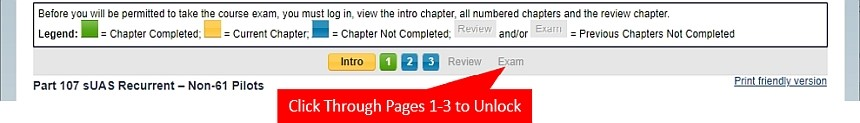
\includegraphics[width=1\linewidth]{images/P107R-unlock} \caption{Make sure you click through to unlock the Exam}\label{fig:p107-unlock}
\end{figure}

\hypertarget{TRUST}{%
\section{TRUST Certificate}\label{TRUST}}

Starting in June 2021, all recreational flyers must pass an aeronautical knowledge and safety test and provide proof of test passage (the TRUST completion certificate) to the FAA or law enforcement (including campus police) upon request. The test is free for everyone and takes 20-30 minutes to complete. The FAA provides education and testing content to FAA Approved Test Administrators of TRUST, who in turn provide the content to recreational flyers for free.

You may take The Recreational UAS Safety Test at any of the administrators found on the FAA's website:
\url{https://www.faa.gov/uas/recreational_fliers/knowledge_test_updates/}

The TRUST is divided into two sections:

\begin{itemize}
\tightlist
\item
  The first section provides you with the information needed to pass the test.
\item
  The second section is a series of multiple choice questions. You cannot fail the test. If you answer a question incorrectly you will be provided with information on why the answer you chose was incorrect and will be promoted to try again.
\end{itemize}

Upon completion of the TRUST you will receive a completion certificate. The certificate never expires however if you lose your certificate you will need to re-take the test and obtain a new certificate. Neither the test administrator, nor the FAA, will maintain personally identifiable information about the recreational flyer so it is not possible to re-print or re-issue your original certificate. We recommend uploading your certificate to UC Drones so that you have a backup copy available.

\hypertarget{what-is-trust}{%
\subsection{What is TRUST?}\label{what-is-trust}}

TRUST is The Recreational UAS Safety Test. It provides education and testing for recreational flyers on important safety and regulatory information. If you fly your drone recreationally under the Exception for Recreational Flyers you must pass the test before you fly - this includes both recreational use and certain academic use-cases.

\begin{center}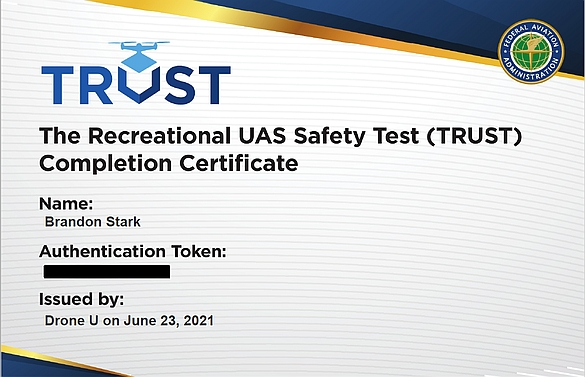
\includegraphics[width=0.5\linewidth]{images/TRUST_cert} \end{center}

\hypertarget{taking-the-trust}{%
\subsection{Taking the TRUST}\label{taking-the-trust}}

You may take the free online test through any of the approved test administrators listed on the FAA's website here: \url{https://www.faa.gov/uas/recreational_fliers/knowledge_test_updates/}. After you complete the TRUST, you will be given the option to download your TRUST certificate and write down your Authentication Token. We recommend uploading your TRUST certificate and entering your Authentication Token into your pilot profile within UC Drones.

\hypertarget{license-FAQ}{%
\section{Frequently Asked Questions}\label{license-FAQ}}

\textbf{When doing an academic activity, which set of regulations is better?}

There are advantages and disadvantages to both scenarios. In many cases, the new `Recreational Operations' may be the fastest path forward for simple, rural flight operations. At the current time, academic UAS activities that plan on flying in certain controlled airspace areas, over occupied structures, within 25 ft of another person, or outside of a reasonably controlled flying site, should proceed with 14 CFR 107 regulations.

\textbf{What does it mean to get approval from the FAA to operate within controlled airspace?}

The FAA is mandating that all controlled airspace access requests for recreational operations be routed through the Low Altitude Authorization Notification Capability system (LAANC) and not by calling the local airport tower. The LAANC system can provide instantaneous authorization via a 3rd party application such as Airmap, KittyHawk, or UASideKick for flight requests below a certain altitude depending on your location.

\textbf{I am planning to fly over a research site that is access controlled and the airspace is uncontrolled, do I need a Drone License?}

Typically not. This common scenario will typically meet the necessary site requirements for Recreational Operations.

\textbf{I am planning to fly along the beach to monitor coastal erosion, do I need a Drone License?}

Unless the beach is to be closed to the public, this scenario will likely require a Drone License.

\textbf{I am planning on flying in the campus quad to test a flight controller, do I need a Drone License?}

If the airspace is uncontrolled (Class G), and the area within the campus is sufficiently cleared and closed to non-participants, then you do not need a Drone License and can get the TRUST certificate. However, there are some parts of some of the UC campuses that are in controlled airspace where a Drone License is required. Please check with your Campus Drone Point of Contact for more information.

\textbf{I do not have a Drone License, can I do a coursework assignment on the use of drones in building inspections with a TRUST certificate?}

You may be able to do some flying with only a TRUST certificate, however, you will not be allowed to fly over a building and must stay at least 25 ft from all non-participants, which may limit your ability to conduct effective analysis.

\textbf{I am a graduate student Teaching Assistant and I would like to teach my students how to fly a drone? Do I need a license? Do the students need a license?}

If the site is sufficiently cleared and closed to non-participants, than everyone may have a chance to learn how to fly a drone with only a TRUST certificate and any instructor may only have a TRUST certificate. However, additional safety precautions may be necessary and as an instructor, you will be responsible for ensuring the safety of the students and the site.

\hypertarget{airspace-info}{%
\chapter{Airspace information}\label{airspace-info}}

When your figuring out where you want to fly, you're typically thinking about your research objectives on the ground. But you must also think about whether or not it will be safe to fly a drone in the airspace at that location. You won't find this information on Google Maps though - you need to check the Airspace Maps or Aviation Charts.

Reading an Airspace Map is not like reading Google Maps - you'll rarely see roads or buildings marked - instead you'll be presented with a whole new set of symbols and strange codes. But they're all very important to convey a dense set of aviation information. Luckily with drones, you won't have to worry about most of it, but there's still some very important pieces of information you need to know.

\begin{notebox}
There's a lot of rules about flying drones and many of them are related to where and how risky. For more information about Airspace Class and their rules, check out the \protect\hyperlink{regulations}{Regulations} and the Reading an Airspace Map pages.

\end{notebox}

\hypertarget{what-is-airspace}{%
\section{What is Airspace?}\label{what-is-airspace}}

The \textbf{Federal Aviation Administration} is in charge of making the rules and regulations for everyone in the United States flying above the ground. While the \textbf{National Airspace System (NAS)} does not have roads or streets like we have on the ground, there are a lot of rules about how to use the airspace correctly for the safety of others\footnote{\url{https://www.faa.gov/about/history/brief_history/}}.

\hypertarget{airspace-classes}{%
\subsection{Airspace Classes}\label{airspace-classes}}

Since aviation works in 3 dimensions, so do the airspace rules. Figure \ref{fig:SUAS-airspace-airspace} gives a side profile of how the airspace is separated into different Classes.

\begin{figure}

{\centering 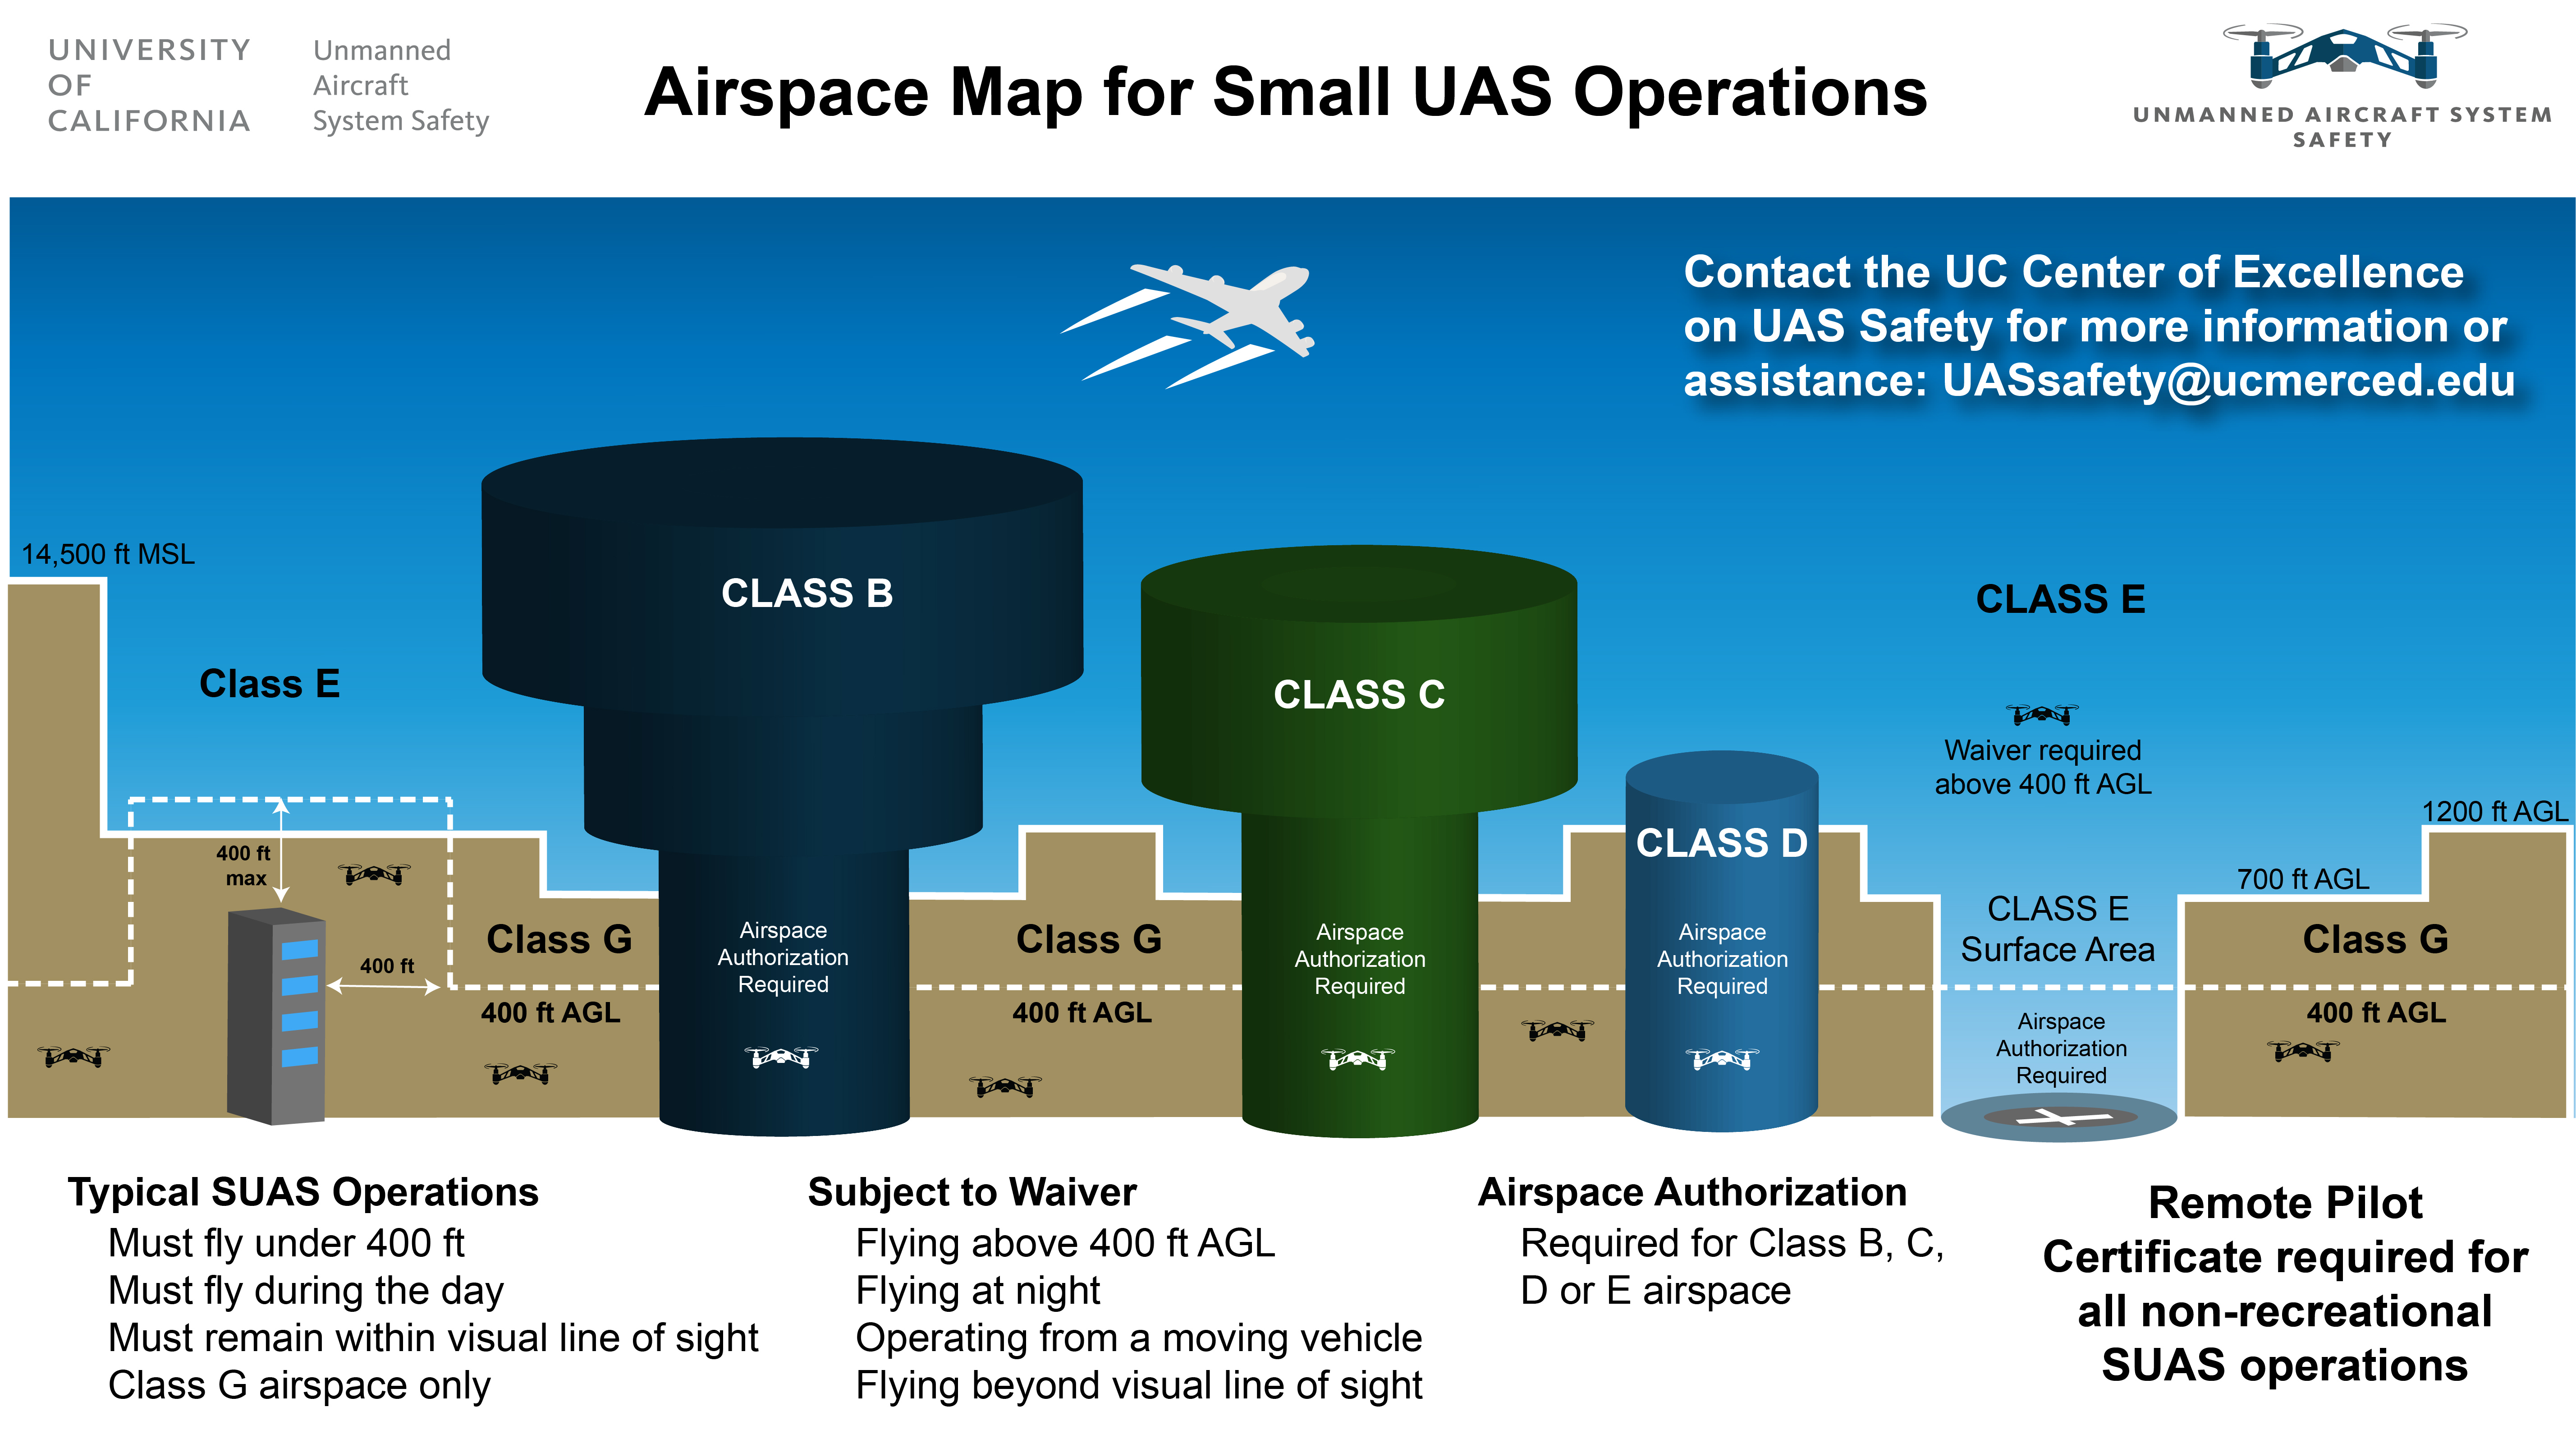
\includegraphics[width=0.9\linewidth]{images/SUAS_airspace_map} 

}

\caption{Small UAS Airspace Rules}\label{fig:SUAS-airspace-airspace}
\end{figure}

\textbf{Class A - Airlines}

Class A is not shown in Figure \ref{fig:SUAS-airspace-airspace}, but exists way up high between 18,000 ft and 60,000 ft above sea level - this is where commercial airliners fly and where our drones should not be. Flying up this high requires special coordination with Air Traffic Control to guide pilots to their destinations.

\textbf{Class B - Big Airports}

Class B airspace is found around the biggest airports in the country - including LAX and SFO. Every Class B airspace is individually tailored as needed to help guide aircraft around these busy areas. This usually involves 2 or more different sized layers at different altitudes - imagine an aircraft taking off from a runway and staying in Class B airspace until it leaves the busiest areas. Given the amount of air traffic around these airports, no one is allowed to fly in Class B airspace unless Air Traffic Control says its ok.

\textbf{Class C - Common Airports}

Class C airspace is found around some of the more common regional airports, such as the Sacramento or Fresno airports. They're busy areas, but not nearly as busy as the major airports, and so they don't need to control as much of the sky as them.

\textbf{Class D - Dinky Airports}

Class D airspace is found around small airports that don't have a lot of commercial airline traffic, mostly catering to private aviation use, such as the airports in Stockton or Palm Springs. But as with Class B and C airspace, no one is allowed to fly within Class D airspace without permission.

\textbf{Class E - the Everywhere Airspace}

Class E airspace is the other airspace that is not part of Class A, B, C, D or G airspace. Fun fact, there are 7 different classifications of Class E airspace. But as a drone pilot, the most important consideration of Class E airspace is when your in the part of Class E airspace at the surface that is designated for an airport. In that case, you'll also need to get permission to fly in that airspace.

\textbf{Class G - The Ground Airspace}

Class G airspace is the airspace at the ground - starting from the ground and going up to either 700 ft or 1200 ft above the ground, depending on location. This is the only airspace that drones are allowed to fly in without getting prior permission. This is true even if you're near an airport. Very small airports, such as those for cropdusters or personal use, do exist in Class G airspace. Though they do not control the airspace near them, you should make sure you stay out of their way.

\hypertarget{what-do-you-need-to-know}{%
\subsection{What do you need to know?}\label{what-do-you-need-to-know}}

There's a lot of information to unpack when looking into airspace information. As you try to figure out if your location will be safe, you'll want to look up:

\begin{itemize}
\tightlist
\item
  Airspace Class
\item
  Nearby Airports, including smaller ones and helipads
\item
  Potential air traffic patterns
\item
  Special Use Airspace - Military Operating Areas, Controlled Firing Ranges, National Security Areas, and Restricted Areas
\item
  Flying altitude limits within certain zones or grids
\item
  Temporary Flight Restrictions or special alerts
\end{itemize}

\hypertarget{how-to-get-airspace-information}{%
\section{How to get Airspace Information}\label{how-to-get-airspace-information}}

So where can you find this information? We recommend two sources:

\begin{itemize}
\tightlist
\item
  Airmap (3rd party application and website)
\item
  Official FAA Sources - VFR Sectional Charts, FAA Facility Maps, TFR/NOTAMs
\end{itemize}

\hypertarget{airmap}{%
\subsection{Airmap}\label{airmap}}

The most comprehensive and easy to use Drone airspace map system is \href{https://app.airmap.com/}{Airmap}. Just type in your address or find your spot on the map, and see whats around you. Airmap is available as both a webpage (Figure \ref{fig:airmap-web}) and as an app for \href{https://apps.apple.com/us/app/airmap-for-drones/id1042824733}{iOS} or \href{https://play.google.com/store/apps/details?id=com.airmap.airmap\&hl=en_US}{Android} (Figure \ref{fig:airmap}).

Once you find your flying spot on the map, you can evaluate many of the airspace issues you need to look for. For example, in Figure \ref{fig:airmap-web}, the selected flying spot is within a grid box within the purple shaded region.
The text box to the bottom left gives a brief explanation - the purple shaded region is MERCED CLASS E2 airspace - meaning that the location is located within the vicinity of the Merced Airport. Any drone flying within any purple of blue shaded region will require permission from the FAA. Class E2 is the least riskiest of the airport managed airspace (also known as controlled airspace), but still will have some airspace risk with occasional planes and helicopters flying above.

\begin{figure}

{\centering 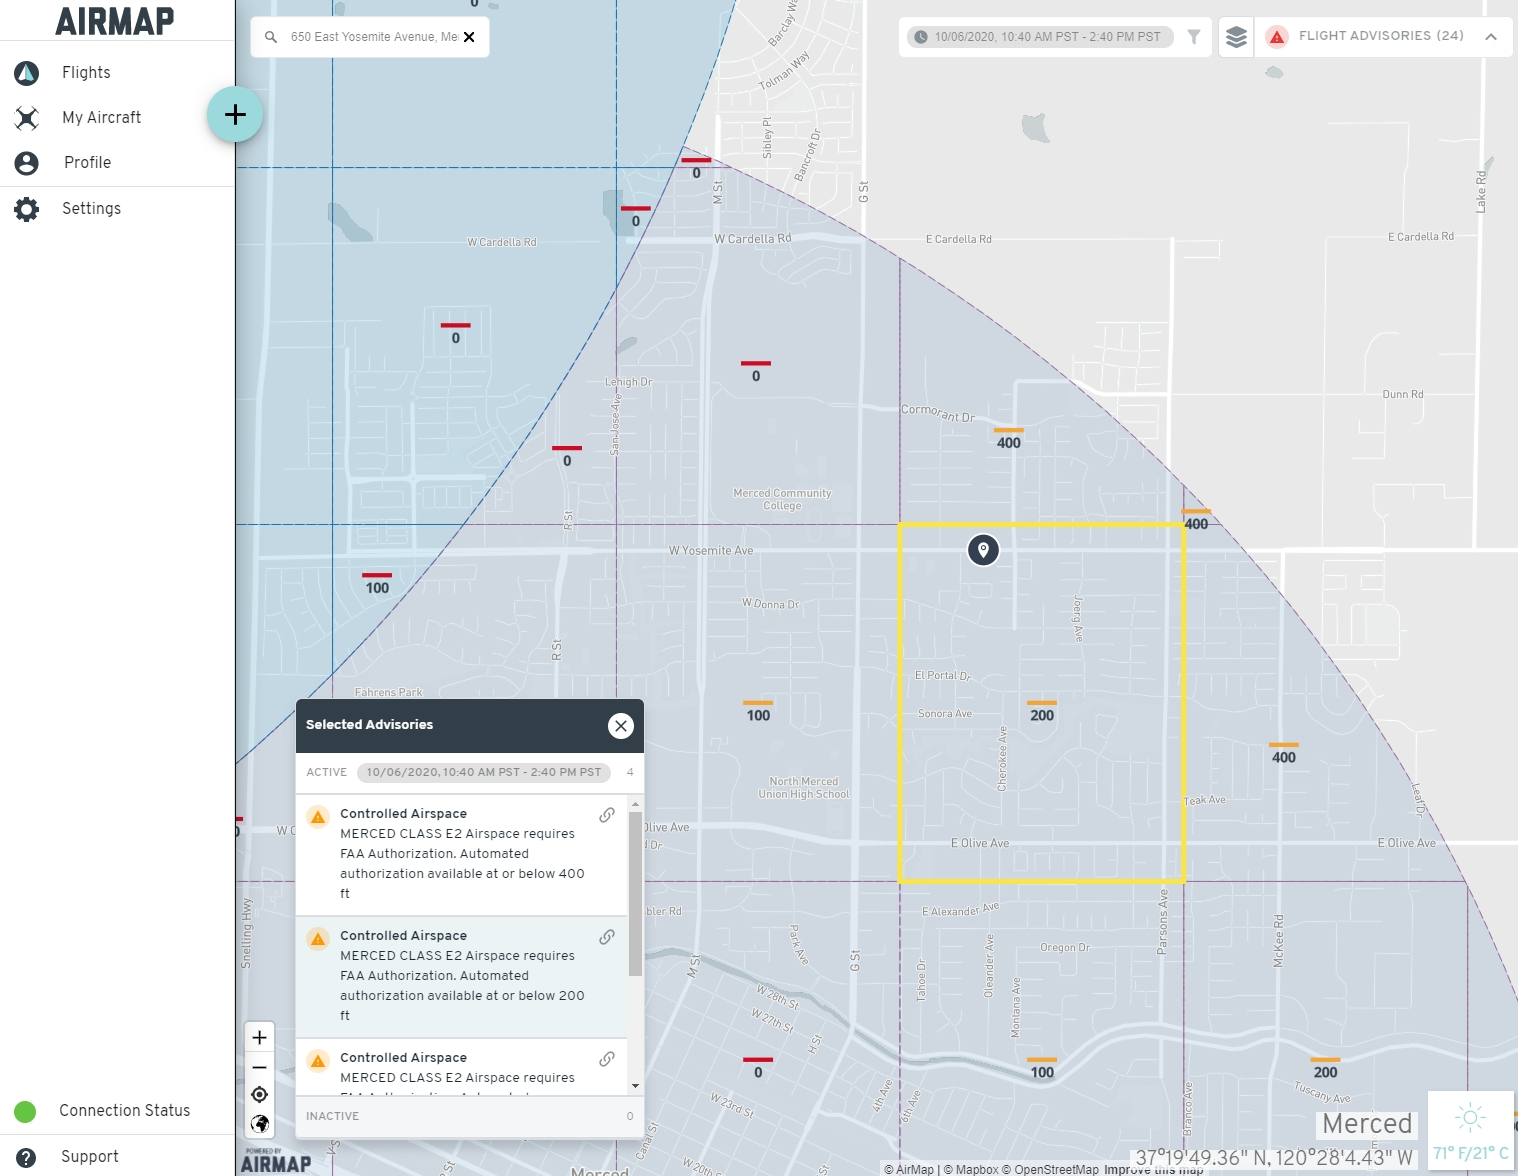
\includegraphics[width=0.85\linewidth]{images/Airmap-webpage} 

}

\caption{Android Airmap Application}\label{fig:airmap-web}
\end{figure}

For requesting permission to fly within a shaded region (controlled airspace), the FAA and the airports have drawn up grids within the shaded regions and labeled each one with a generally safe upper limit for flying. Within the highlighted grid in Figure \ref{fig:airmap-web}, this limit is 200 ft. If you ask the FAA for permission to fly up to 200 ft, you will always be given approval. In general, the farther away you are from the runway, the higher the altitude you will be allowed to fly. But that's not always the case - you'll notice, there are a couple of grids that are marked with a 0 - and yes, that means that the generally safe flying altitude is 0 ft.

\begin{notebox}
Need to get FAA permission to fly in one of these areas, head over \protect\hyperlink{LAANC}{here}

\end{notebox}

What if you need to fly higher than the altitude listed? If you have a drone pilot license, you may ask the FAA for permission - but it is not guaranteed to be approved. Obtaining permission for flights above the listed altitude can be tricky, so we recommend reaching out to us at \href{mailto:UASsafety@ucmerced.edu}{\nolinkurl{UASsafety@ucmerced.edu}} and we'll be happy to walk you through the process. Reach out to us early - the FAA can take 5-10 days to grant approval so you want to start this process early.

Airmap also does a good job of depicting other airspace issues, such as Special Use Airspace and National Security Areas - marked in red as in Figure \ref{fig:airmap}. Selecting the AIRMAP Recommended Guidelines layer will also show all the helipads and minor airports that are not normally shown on an airspace map. This can be critically important - low flying helicopters and cropdusters that fly out of these unmarked airports are among the most pressing airspace concerns.

\begin{notebox}

Make sure you click on the `Layers' Icon next to the Flight Advisories - this allows you to turn on/off different information. For most operations, we recommend selecting the following sets of information:

\begin{itemize}
\tightlist
\item
  FAA Part 107 Certified
\item
  AIRMAP Recommend Guidelines
\item
  Restricted and Special Use Airspace
\item
  National Parks Public Use Limits
\item
  NOAA Regulated Overflight Zones
\item
  Fish and Wildlife Service Lands Use Limits
\item
  Wilderness Areas Use Limits
\end{itemize}

\end{notebox}

\begin{figure}

{\centering 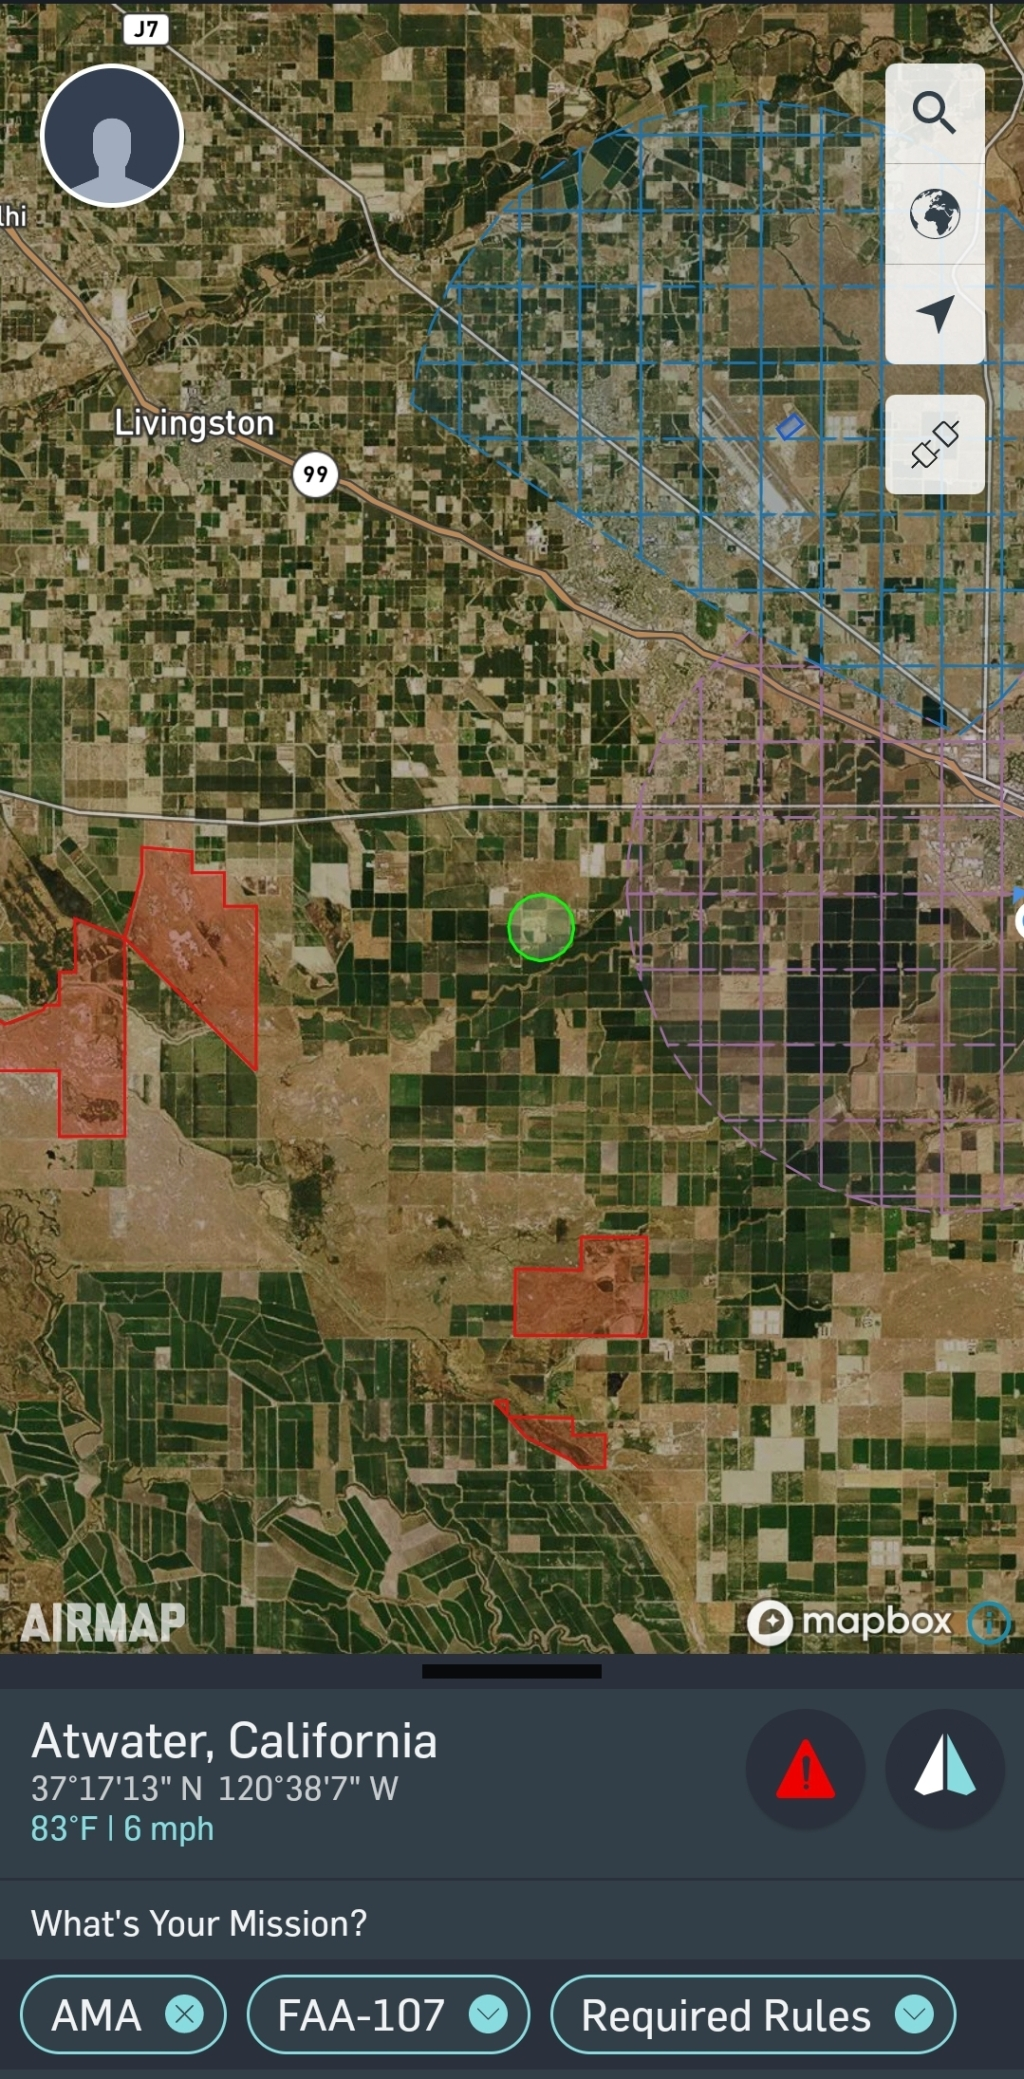
\includegraphics[width=0.5\linewidth]{images/Airmap-Android} 

}

\caption{Android Airmap Application}\label{fig:airmap}
\end{figure}

\hypertarget{the-importance-of-up-to-date-airspace-information}{%
\subsection{The importance of up-to-date Airspace Information}\label{the-importance-of-up-to-date-airspace-information}}

Having the most up-to-date airspace information on hand can make all the difference between having a safe flight and a risky one. One of the advantages of Airmap is that it will also display a number of Temporary Flight Restrictions and Notices to Airman. Especially in California, there are a number of these that we should always keep an eye on:

\begin{itemize}
\tightlist
\item
  \textbf{Disneyland} - Due to National Security Risks, the FAA has banned all aircraft from flying under 3000 ft within 3 miles of Disneyland. This essentially also bans all drones in the area as well.\\
\item
  \textbf{Major League Baseball}, \textbf{National Football League} and \textbf{Division 1 College Football} Regular and Post-Season Games - Similarly to the Disneyland restriction, the FAA has banned all aircraft from flying under 3000 ft within 3 miles of any these games. The ban starts at 1 hour before the games begin to 1 hour after the game ends.\\
\item
  \textbf{Wildfire and other Natural Disasters} - Whenever there is a major catastrophe, keep an eye out for Temporary Flight Restrictions. These will often be very large and prolonged to allow emergency services (firefighting aircraft, medical support, etc) to have priority in these areas. Never fly your drone in a manner that could interfere with emergency services - it is both a Federal offense and a State offense.\\
\item
  \textbf{US President and Vice-President Travel} - The President (30 mile) and Vice-President (5 mile) travel with their own FAA flight restriction zones, similarly prohibiting all aircraft from flying under 3000 ft within their zones.
\end{itemize}

\begin{notebox}
As with most drone related rules and regulations, there are nuances and exceptions to TFRs and NOTAMs. If you have a pressing need to operate within a TFR, reach out to us at \href{mailto:UASsafety@ucmerced.edu}{\nolinkurl{UASsafety@ucmerced.edu}} to discuss.

\end{notebox}

\hypertarget{official-faa-sources}{%
\subsection{Official FAA Sources}\label{official-faa-sources}}

Using Airmap is one of the easiest methods for looking up most of the airspace issues. However, it's not always the most detailed nor is it the official source of information. The official sources of information is spread across a handful of different sites:

\begin{itemize}
\tightlist
\item
  Official source of airspace information - \href{https://www.faa.gov/air_traffic/flight_info/aeronav/digital_products/vfr/}{FAA Sectional Charts}
\item
  Official source of altitude grid information - \href{https://faa.maps.arcgis.com/apps/webappviewer/index.html?id=9c2e4406710048e19806ebf6a06754ad}{UAS Facility Maps}
\item
  Official source of TFR or NOTAMS - \href{https://notams.aim.faa.gov/notamSearch/nsapp.html\#/}{FNS NOTAM Search}
\end{itemize}

\begin{notebox}
Always check multiple sources - you never know when one source omits an important piece of information. For example, Figure \ref{fig:facility-map} is the default view of Orange County of the UAS Facility Maps, but its doesn't depict one very critical flight restriction.

\end{notebox}

\hypertarget{faa-sectional-charts}{%
\subsubsection{FAA Sectional Charts}\label{faa-sectional-charts}}

\begin{figure}
\centering
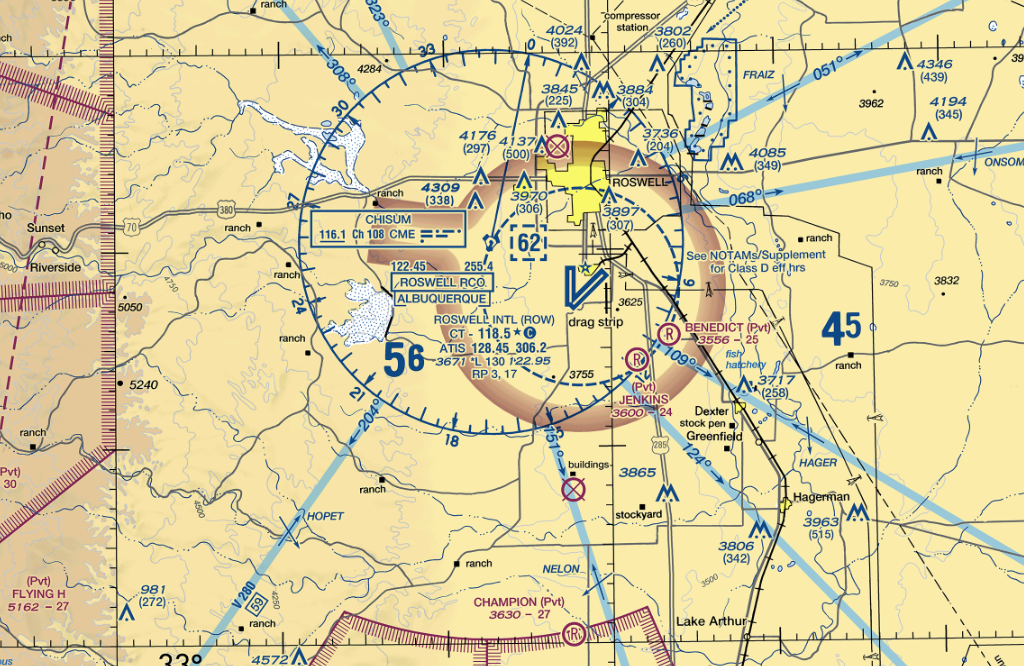
\includegraphics{images/FAA-VFR.png}
\caption{FAA sectional chart}
\end{figure}

Getting information on a specific area's airspace classification has never been easier. The FAA has region specific sectional charts located \href{https://www.faa.gov/air_traffic/flight_info/aeronav/digital_products/vfr/}{here}.

\hypertarget{uas-facility-maps}{%
\subsection{UAS Facility Maps}\label{uas-facility-maps}}

\begin{figure}

{\centering 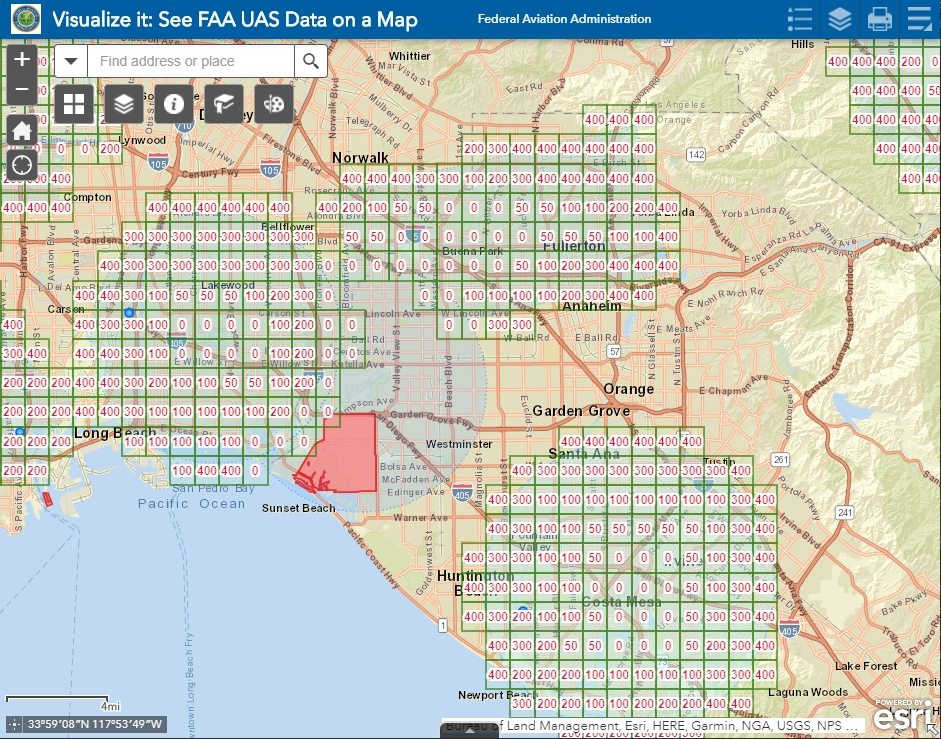
\includegraphics[width=0.9\linewidth]{images/facility-map} 

}

\caption{UAS Facility Map}\label{fig:facility-map}
\end{figure}

UAS Facility Maps show the maximum altitudes around airports where the FAA may authorize drone operations without additional safety analysis. Grids marked in Green are LAANC (Low Altitude Authorization and Notification Capability) enabled - More on that in \protect\hyperlink{ch-LAANC}{LAANC Authorization}.

\hypertarget{notam-or-notice-to-airman}{%
\subsection{NOTAM or Notice To Airman}\label{notam-or-notice-to-airman}}

\begin{figure}
\centering
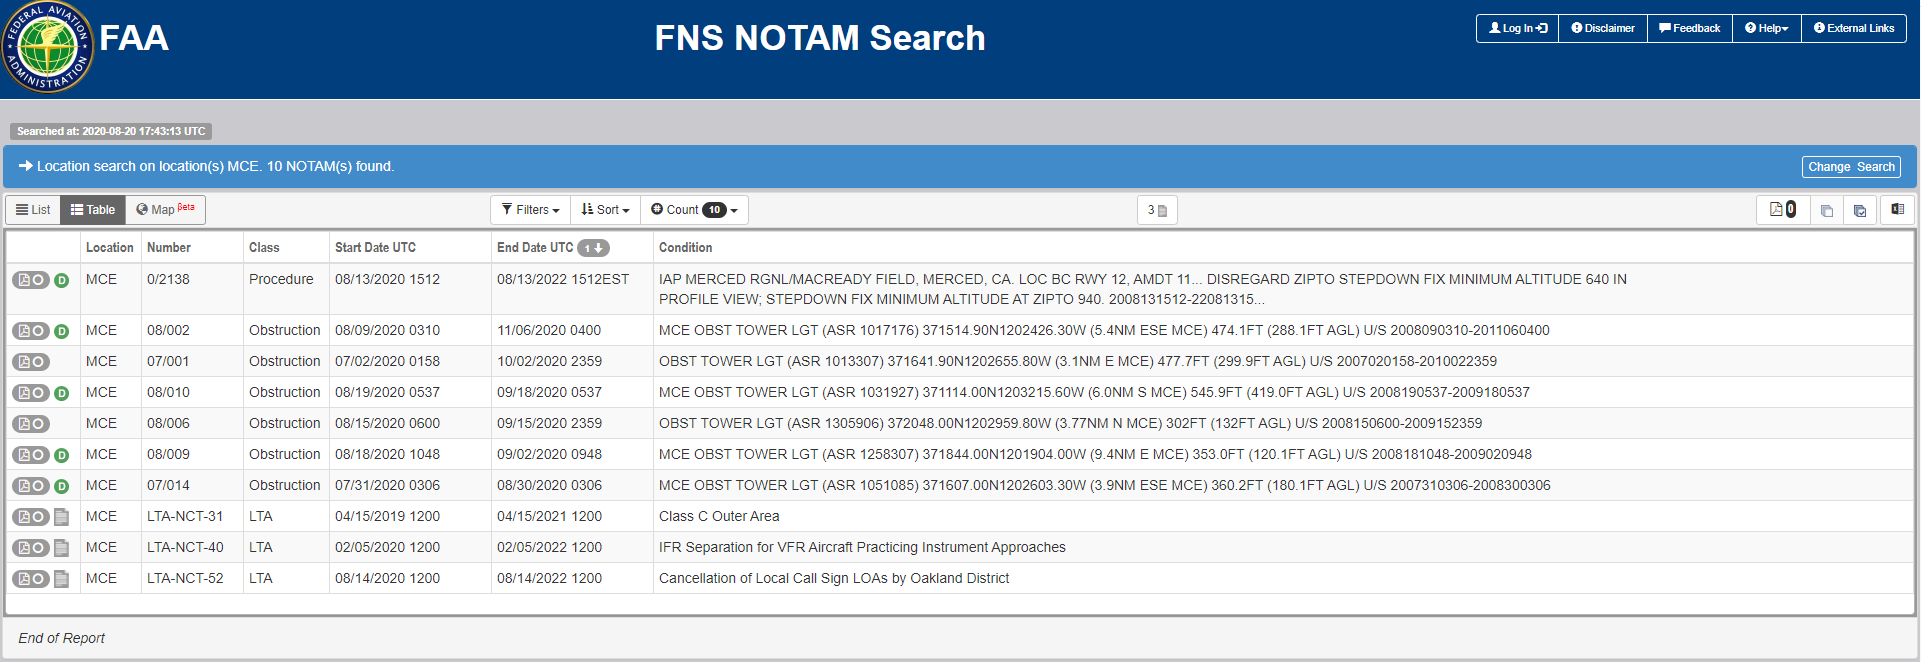
\includegraphics{images/FAA-Notam.png}
\caption{FAA NOTAM (Notice to Airman)}
\end{figure}

A NOTAM or Notice to Airman, is a notice that pertains to the establishment, change or condition of any facility, service or procedure of a specific location. The information is not known far enough in advance to be publicized by any other means therefore ensuring there are no active NOTAMS in the area you will be flying in is essential to the safety of yourself and others. It is important to keep in mind that NOTAMS can be put up at a moments notice.

\hypertarget{other-sources}{%
\subsection{Other Sources}\label{other-sources}}

Two other useful sources of information are \href{https://skyvector.com/}{Skyvector} and the B4UFly App (\href{https://apps.apple.com/us/app/b4ufly/id992427109}{iOS} and \href{https://play.google.com/store/apps/details?id=gov.faa.b4ufly2\&hl=en}{Android}).

\hypertarget{skyvector}{%
\subsubsection{SkyVector}\label{skyvector}}

\begin{figure}

{\centering 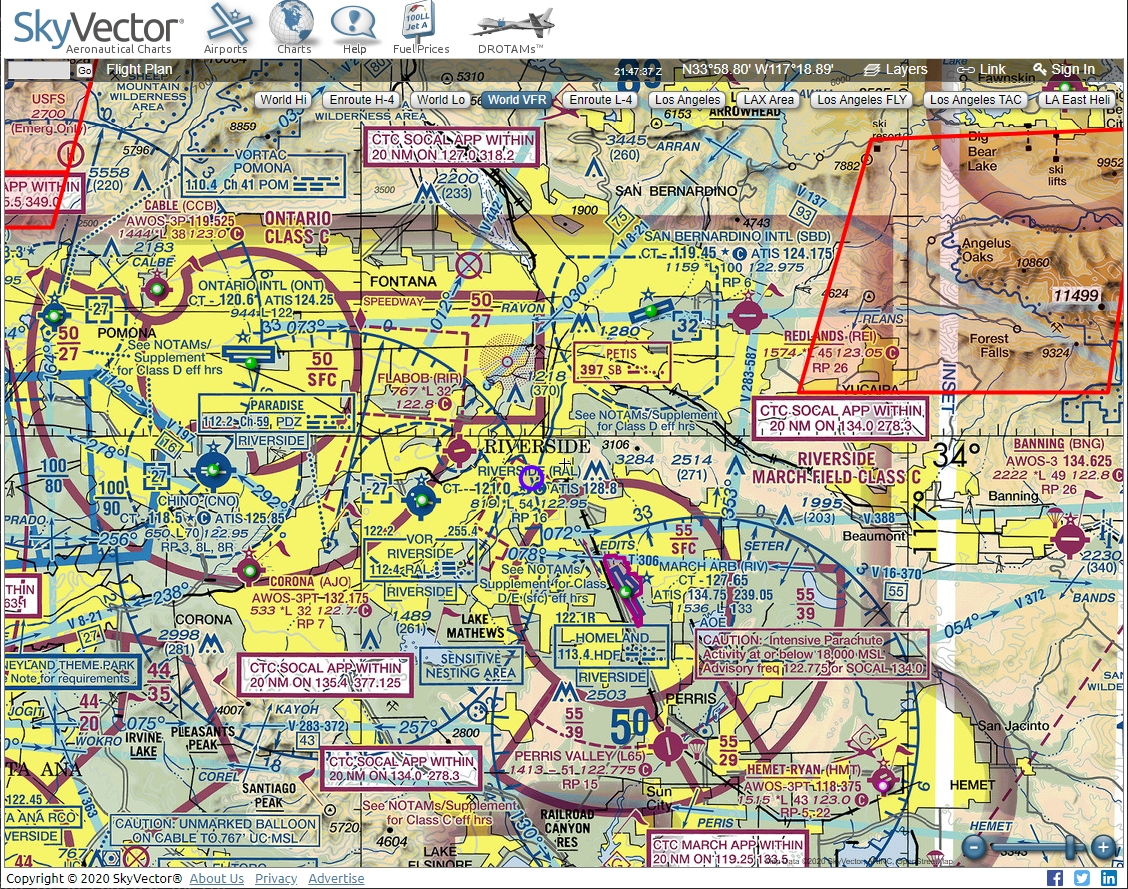
\includegraphics[width=0.9\linewidth]{images/skyvector} 

}

\caption{SkyVector - VFR Chart viewer with TFRs}\label{fig:skyvector}
\end{figure}

SkyVector is a manned aviation tool that allows users to view the FAA Sectional Charts (also known as VFR charts) as well as a wide range of other layers, including TFRs and IFR approaches. While most of the information will be overwhelming for the beginning drone pilot, the basic VFR charts are still a great resource.

\hypertarget{b4ufly-app}{%
\subsubsection{B4UFly App}\label{b4ufly-app}}

The B4UFly App has been redesigned by Aloft (formerly kittyhawk.io) and now includes a lot of good information. It also now includes an integration with the Aloft App to review FAA facility maps and file LAANC requests.

\href{https://www.faa.gov/uas/recreational_fliers/where_can_i_fly/b4ufly/}{B4UFly App}

\begin{figure}

{\centering 
\includegraphics[width=0.5\linewidth]{images/B4UFLYlogo} 

}

\caption{B4UFly}\label{fig:b4ufly}
\end{figure}

\hypertarget{airspace-regulations}{%
\subsection{Airspace Regulations}\label{airspace-regulations}}

On this page, we're only looking at how to get the most basic of airspace information. But obviously, there's a deeper level of knowledge to be studied when it comes to airspace regulations. You'll find more information on the UAS Regulations and Learning About Airspace page, but for now, you can take a quick look at Figure \ref{fig:SUAS-sim-regs} below.

\begin{figure}

{\centering 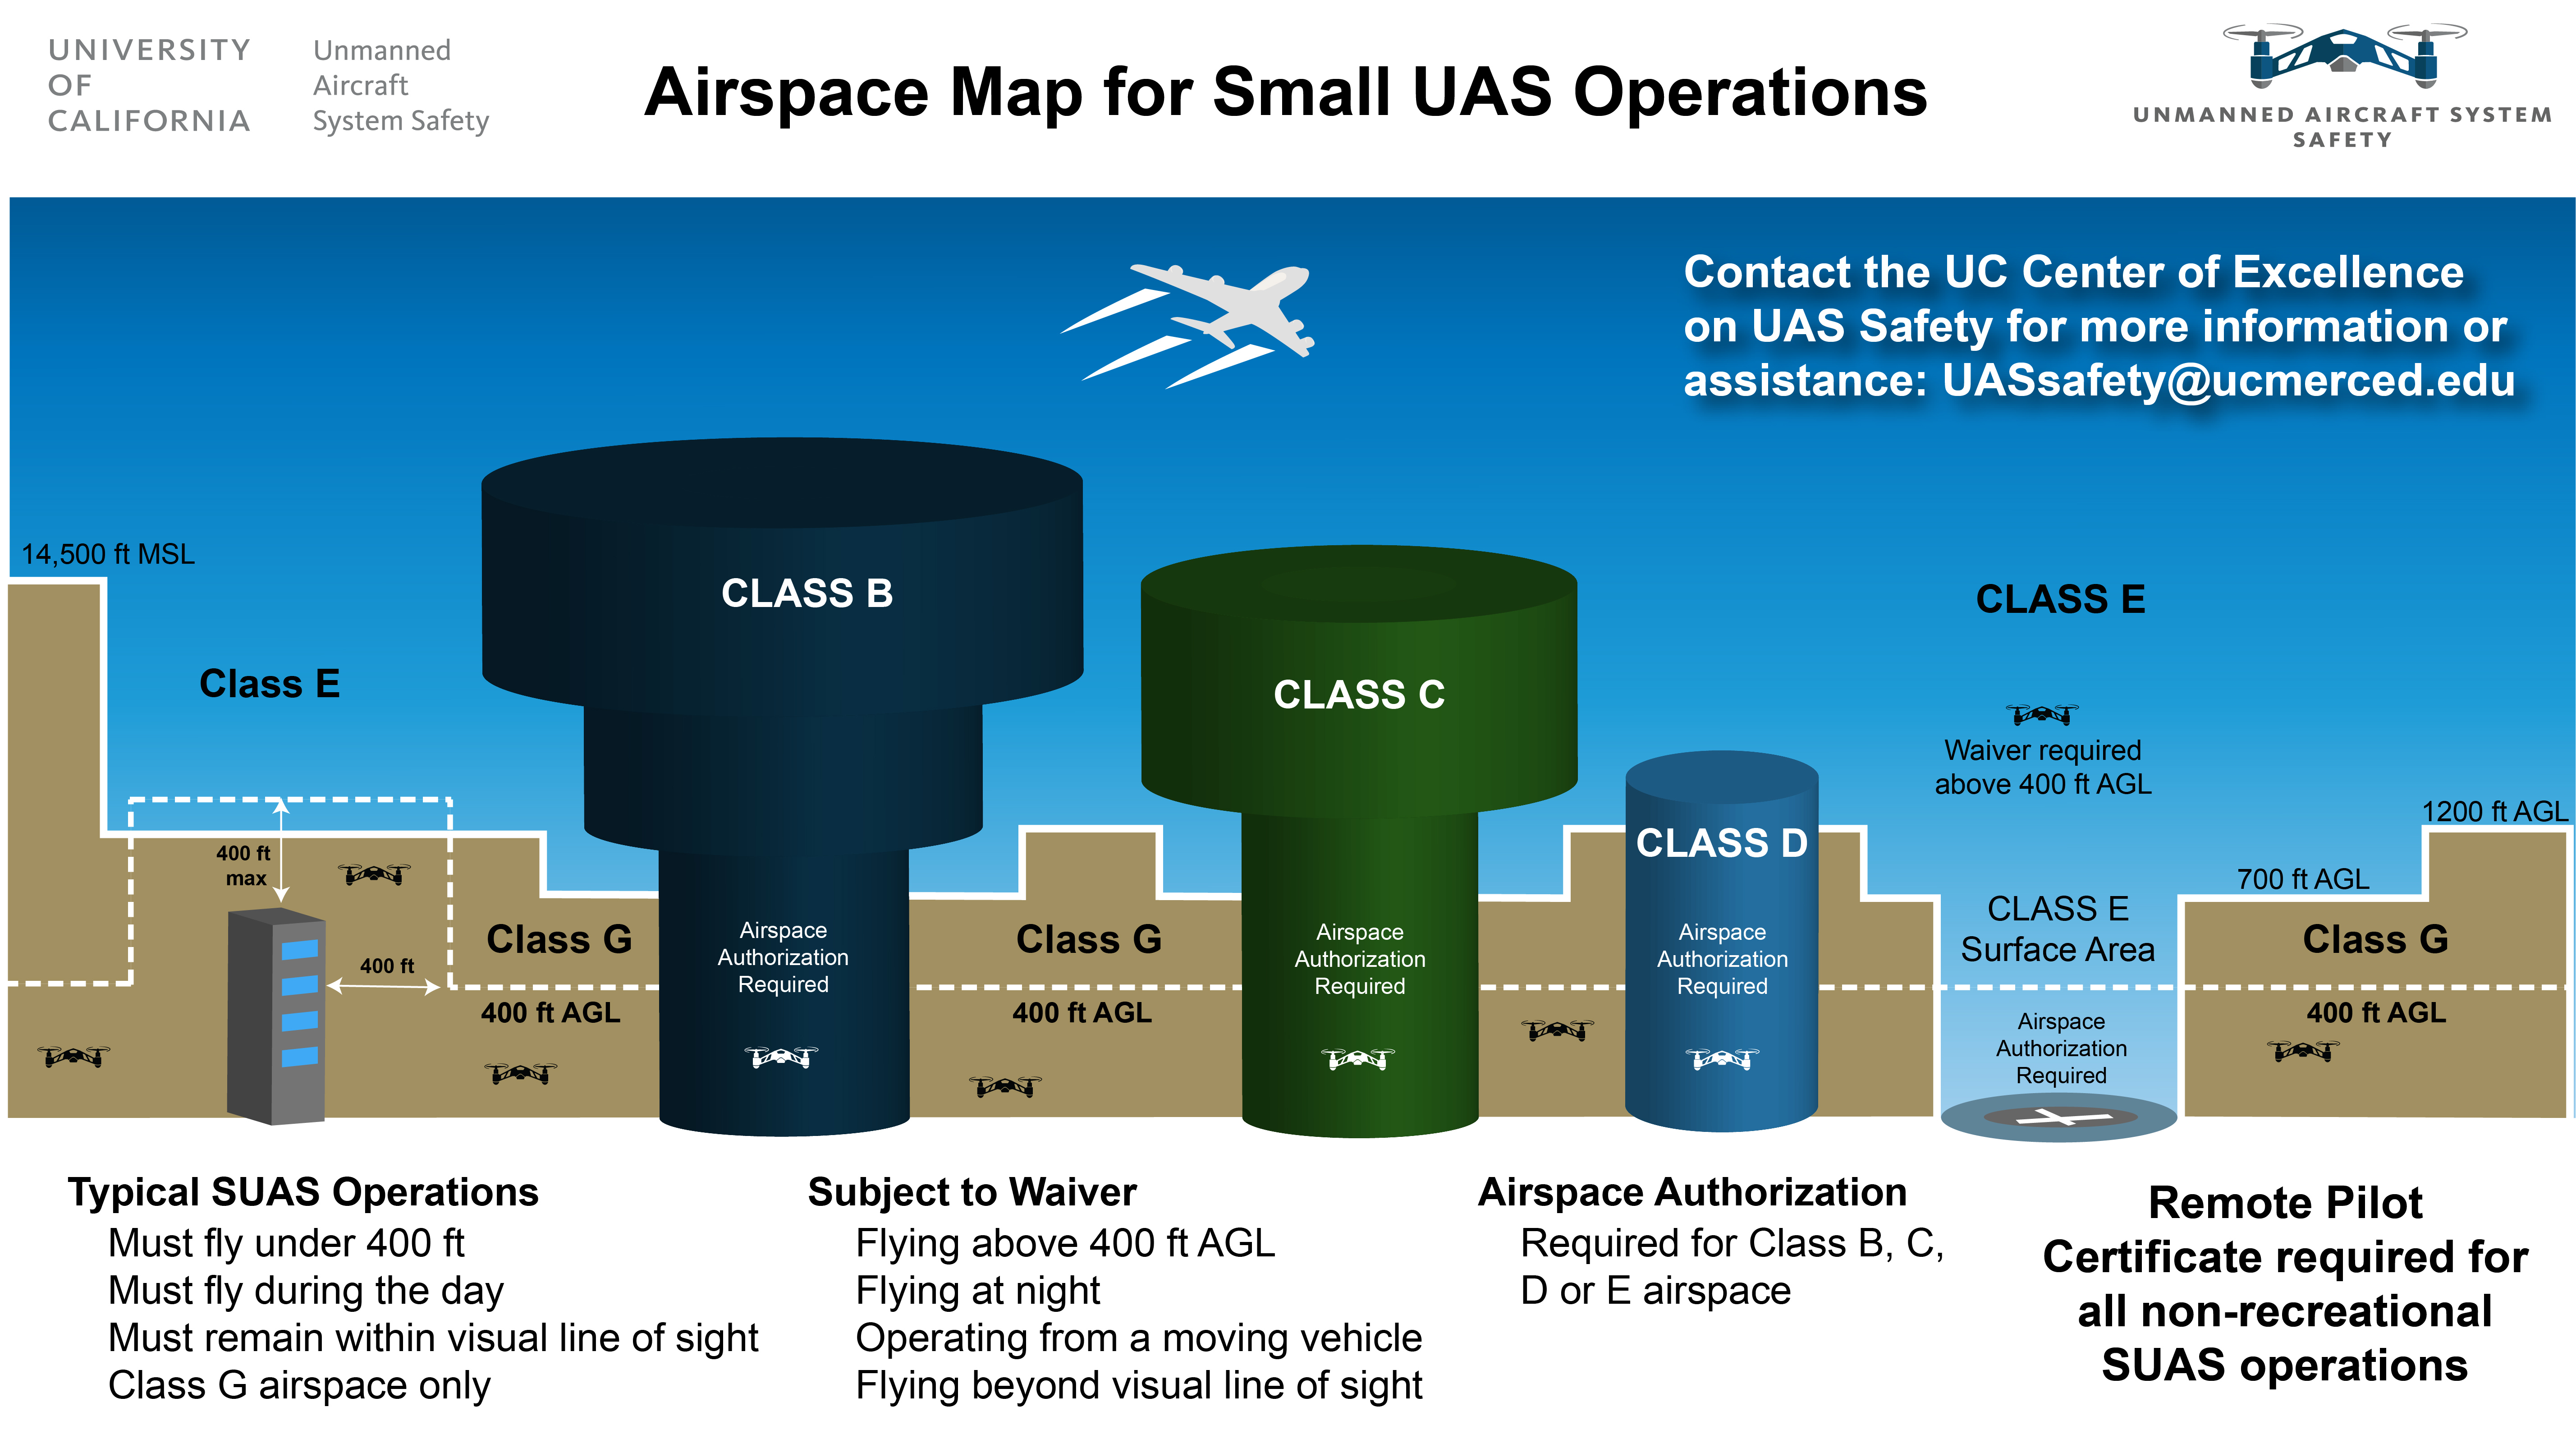
\includegraphics[width=0.9\linewidth]{images/SUAS_airspace_map} 

}

\caption{Small UAS Airspace Rules}\label{fig:SUAS-sim-regs}
\end{figure}

\hypertarget{LAANC}{%
\section{LAANC Authorization}\label{LAANC}}

In order to get FAA authorization to fly in controlled airspace, you typically will need to file a request through a system called ``LAANC'' (pronounced lance)

\begin{itemize}
\tightlist
\item
  If you plan on flying below the Facility Map altitude maximum, authorization will be instantaneous.
\item
  If you want to request flying above the Facility Map altitude maximum, you'll need a Part 107 license and you'll need to make a safety case within your request. Flight requests are automatically denied if they have not been resolved 24 hours prior to flight, so we recommend filing a request at least 1 week in advance.
\end{itemize}

\hypertarget{using-airmap}{%
\subsection{Using AirMap}\label{using-airmap}}

One of our favorite programs to use for simple and free airspac authorizations is AirMap. The process is relatively straightfoward. Create an account, input your pilot and aircraft information, then find a place to fly. Point to a spot on the map, draw a polygon or even just a line to describe your flight area then submit your flight plan. It'll go straight to the FAA, or if manual approval by the tower is necessary, it'll go straight to the tower.

For more information on how to use Airmap, check out their support information here:

\href{https://support.airmap.com/hc/en-us/articles/360030924511-How-to-apply-for-Authorization}{How to apply for Authorization}

\hypertarget{tips-tricks}{%
\subsection{Tips \& Tricks}\label{tips-tricks}}

\begin{itemize}
\item
  \textbf{Need to draw a polygon using a satellite map?}

  Try this:

  \begin{itemize}
  \tightlist
  \item
    Go to \url{https://geoman.io/geojson-editor} and draw your polygon with satellite map on. Export to a GeoJSON text file
  \item
    Upload the GeoJSON file to Airmap using the `cloud' button underneath the polygon.
  \item
    The outline should now cover the right area and you file as normal
  \end{itemize}
\end{itemize}

\hypertarget{UCdrones}{%
\chapter{UC Drones}\label{UCdrones}}

\href{http://ehs.ucop.edu/drones}{UC Drones} is a one-stop shop for drone oversight and management for the University of California system. It is designed with the goal to develop a culture of safety and accountability in the use of drone by providing a unified portal for 1 ) enabling users be kept aware with regulatory compliance obligations, safety guidelines and best practices, 2) documenting drone activity through flight requests and reporting, and 3) tracking UC drone operations and safety metrics.

The use of \href{http://ehs.ucop.edu/drones}{UC Drones Web App} is UC UAS Policy compliant. However, it is not the only means of UC UAS Policy compliance. \textbf{If an alternative means of UC UAS Policy is needed or requested, please contact your campuses' drone Point of Contact.}

\href{http://ehs.ucop.edu/drones}{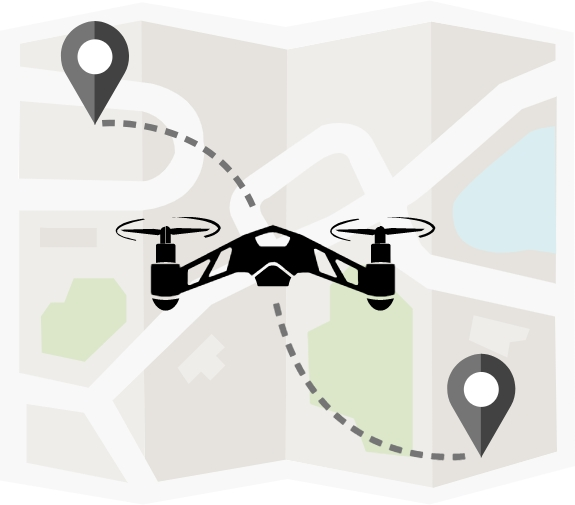
\includegraphics{images/UCDrones_logo.jpg}}

\hypertarget{UCdrones-login}{%
\section{Logging into UC Drones}\label{UCdrones-login}}

The UC Drones Web App is part of the UC Safety suite of apps for lab safety, occupational health and risk management.

The UC Drones homepage can be found at \url{http://ehs.ucop.edu/drones} or through the Risk \& Safety Solutions platform

\begin{figure}

{\centering 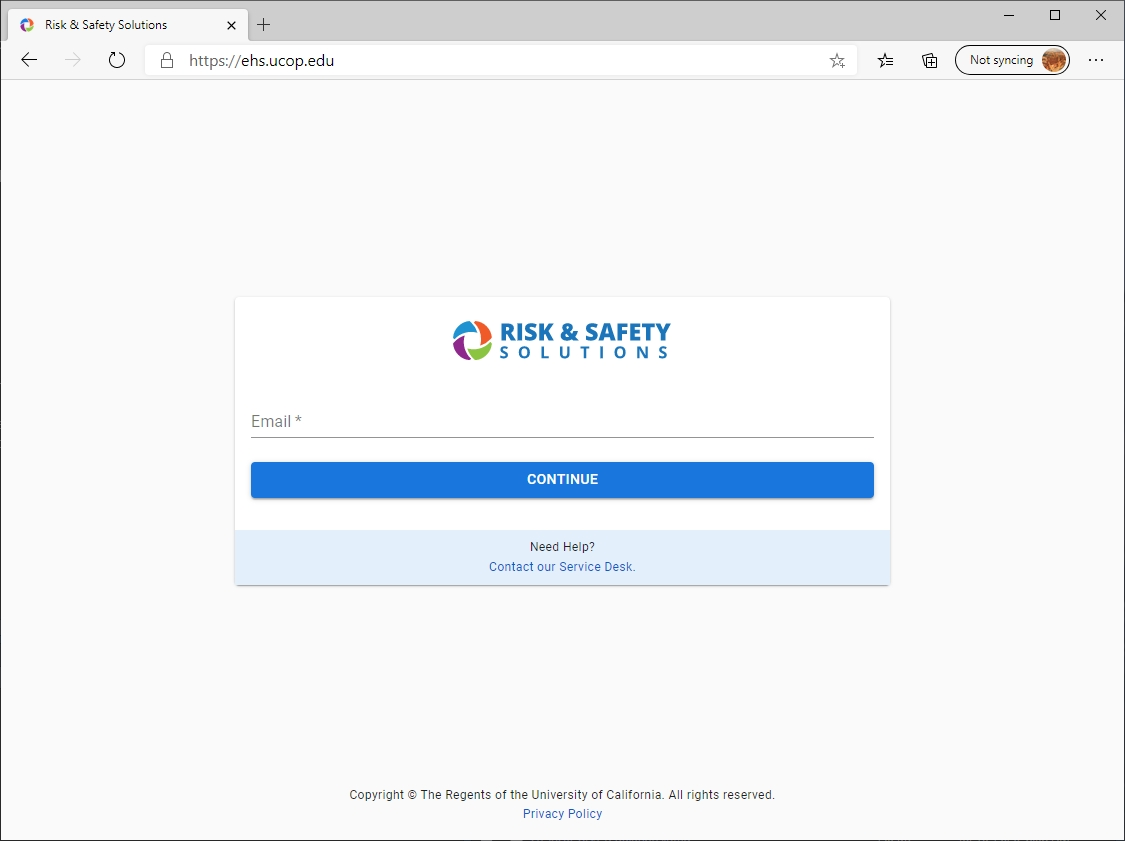
\includegraphics[width=0.85\linewidth]{images/RSS_home} 

}

\caption{Risk and Safety Solutions Login}\label{fig:rss-web}
\end{figure}

\begin{enumerate}
\def\labelenumi{\arabic{enumi}.}
\tightlist
\item
  The UC Safety suite of apps can be found at \url{https://ehs.ucop.edu/}

  \begin{enumerate}
  \def\labelenumii{\arabic{enumii}.}
  \tightlist
  \item
    The homepage will look similar to the image shown above:
  \item
    When you enter your campus email address, it will redirect you to your campus Single Sign On.
  \item
    Once logged in, you'll be taken to the RSS Platform Dashboard. On the left, click on `More Apps' and you'll find `Drones' listed
  \end{enumerate}
\item
  You can login directly from \url{http://ehs.ucop.edu/drones}

  \begin{enumerate}
  \def\labelenumii{\arabic{enumii}.}
  \tightlist
  \item
    If you're not logged in already, you'll be redirected to login through your campus Single Sign On
  \end{enumerate}
\end{enumerate}

\begin{figure}

{\centering 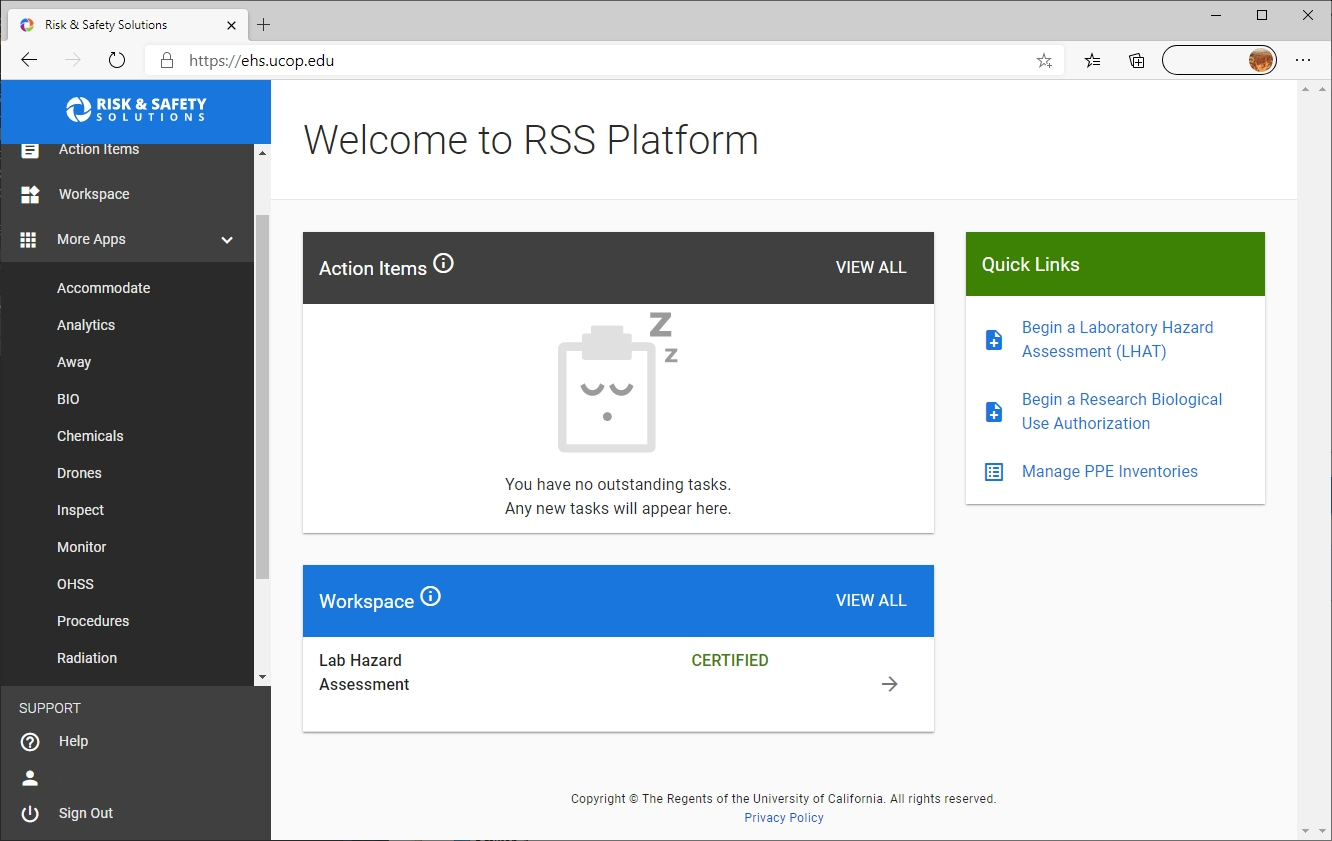
\includegraphics[width=0.85\linewidth]{images/RSS_apps} 

}

\caption{Risk and Safety Solutions Dashboard}\label{fig:rss-dash}
\end{figure}

\hypertarget{UCDrones-home}{%
\section{UC Drone Home Page}\label{UCDrones-home}}

The UC Drone Safety Home Page allows users to manage their drone flights, aircraft and their pilot information.

\begin{figure}

{\centering 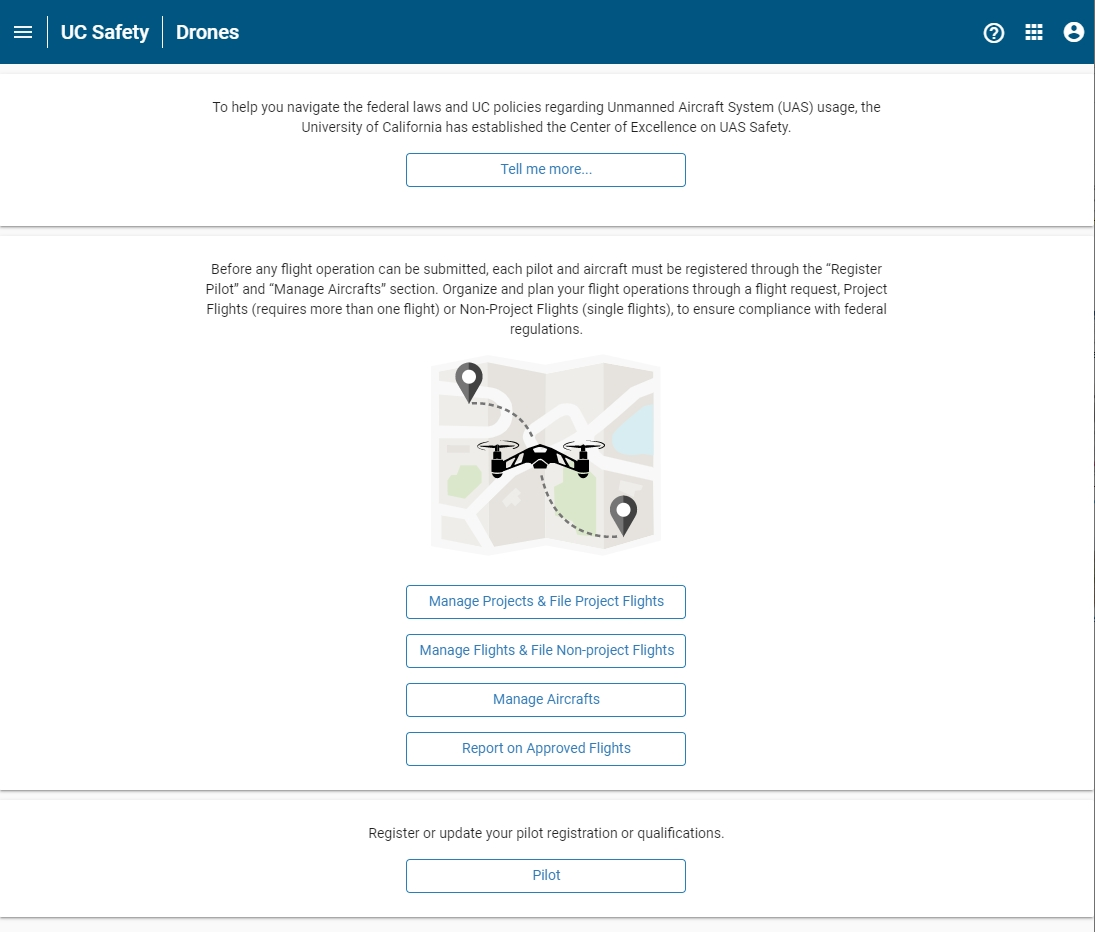
\includegraphics[width=0.85\linewidth]{images/UCDrones_Home} 

}

\caption{UC Drones Home Page}\label{fig:UCDrones-home}
\end{figure}

\hypertarget{projects-and-flights}{%
\subsection{Projects and Flights}\label{projects-and-flights}}

Within UC Drones, you have two types of Requests available:

\begin{itemize}
\tightlist
\item
  Flight Projects
\item
  Individual Flights
\end{itemize}

\hypertarget{flight-project}{%
\subsubsection{Flight Project}\label{flight-project}}

A Flight Project comprises of multiple sets of drone flights over defined period of time (up to 1 year) at a single area of operation. The Flight Project as a whole can be reviewed and approved within the app, rather than reviewing each flight. All flight requests under an approved Flight Project are automatically approved and an email notice is sent to the local drone Point of Contact.

\textbf{Example Flight Projects}

\begin{itemize}
\tightlist
\item
  Recurrent flight operations on field stations that do not require scheduling
\item
  Regular flight activity in access-controlled construction sites
\item
  Ad-hoc flights by NRS staff or researchers
\item
  Weekly flights on the user's farm plots
\item
  A three-day workshop on campus where the location has been reserved
\end{itemize}

A Flight Project may not be edited once it has been approved. A separate Flight Project must be submitted if a new pilot is desired.

\hypertarget{individual-flight-request}{%
\subsubsection{Individual Flight Request}\label{individual-flight-request}}

An individual Flight Request comprises of one or more drone flights on a single day. Each Flight Request is reviewed individually, typically to address local issues such as campus safety, scheduling or privacy concerns.

\textbf{Example Individual Flight Requests}

\begin{itemize}
\tightlist
\item
  Any site that the field manager requires prior approval for scheduling or wildlife considerations
\item
  Athletic or recreational fields that require scheduling
\item
  On-campus public areas without additional mitigation protocols or safety hazard analysis.
\item
  Special operations -- flying at night, flying above 400 ft AGL, etc
\end{itemize}

\hypertarget{manage-aircrafts}{%
\subsection{Manage Aircrafts}\label{manage-aircrafts}}

The Manage Aircrafts page allows the user to add aircraft for use in the UC Drones web app or edit their existing aircraft. All aircraft registered at a campus will be visible to all, but only the Responsible Person may edit the entry.

\hypertarget{report-on-approved-flights}{%
\subsection{Report on Approved Flights}\label{report-on-approved-flights}}

The Report on Approved Flights page lists all of the Approved Flights that the user is listed as either a pilot or the point of contact. The user can select any of the approved flights and Create a Post-Flight Report to complete the UC Drone Policy process.

\hypertarget{pilot}{%
\subsection{Pilot}\label{pilot}}

The Pilot page allows the user to enter in their pilot information, including their certificate number and any additional certifications as attachements.

\hypertarget{UCDrones-project}{%
\section{Submitting a Flight Project}\label{UCDrones-project}}

A Flight Project comprises of multiple sets of drone flights over defined period of time (up to 1 year) at a single area of operation per aircraft. The Flight Project as a whole can be reviewed and approved within the app, rather than reviewing each flight. All flight requests under an approved Flight Project are automatically approved and an email notice is sent to the local Drone Point of Contact.

\textbf{Example Flight Projects}

\begin{itemize}
\tightlist
\item
  Recurrent flight operations on field stations that do not require scheduling
\item
  Regular flight activity in access-controlled construction sites
\item
  Ad-hoc flights by NRS staff or researchers
\item
  Weekly flights on the user's farm plots
\item
  A three-day workshop on campus where the location has been reserved
\end{itemize}

A Flight Project may not be edited once it has been approved. A separate Flight Project must be submitted if a new pilot is desired.

\hypertarget{manage-projects-page}{%
\subsection{Manage Projects Page}\label{manage-projects-page}}

The Manage Project page lists all of the Flight Projects that the user is listed as the Point of Contact or as one of the Pilots.

\begin{figure}

{\centering 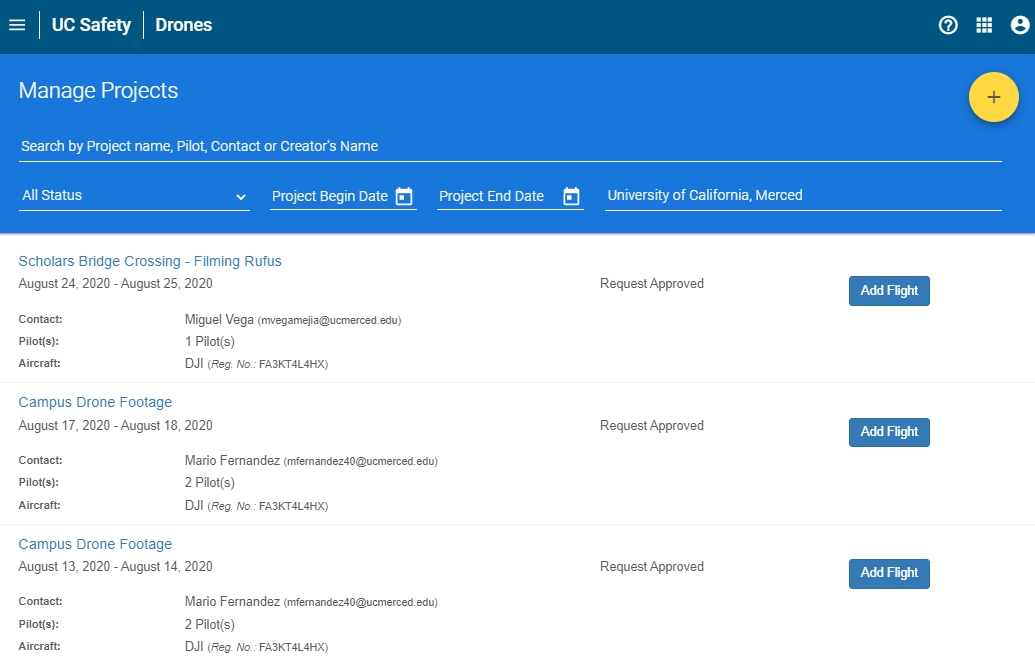
\includegraphics[width=0.85\linewidth]{images/UCDrones_manage_project} 

}

\caption{UC Drones Manage Projects}\label{fig:UCDrones-project}
\end{figure}

The list of projects is searchable by

\begin{itemize}
\tightlist
\item
  Name of Project
\item
  Name of Pilot, Point of Contact or Creator
\item
  Status of Project Request: Draft, Pending Review, In Review, Request Reviewed, or Request Denied
\item
  Date Range to Search (Project Begin Date - Project End Date)
\end{itemize}

Each project is listed with the Project Name, the project date range, status of Project request, point of contact, the number of pilots associated with the Project and the aircraft for the project.

\hypertarget{project-request-form}{%
\subsection{Project Request Form}\label{project-request-form}}

To submit a Project request, go to the Manage Projects Page (Figure \ref{fig:UCDrones-project}) and click on the yellow + (plus) button to go to the Project Information Page to start the request.

\hypertarget{enter-project-information}{%
\subsubsection{Enter Project Information}\label{enter-project-information}}

The following interactive module provides a breakdown on how to fill out a Project Request. The module requires a browser compatible with HTML5. If you are having difficulty viewing the interactive module, please contact us at \href{mailto:UASsafety@ucmerced.edu}{\nolinkurl{UASsafety@ucmerced.edu}}.

Please visit the webpage for the interactive module on how to fill out a Project Request.

\begin{enumerate}
\def\labelenumi{\arabic{enumi}.}
\item
  \textbf{Enter Aircraft}

  Enter either the Aircraft FAA registration number, or search by the Aircrafts nickname. All aircraft at your campus will be visible, so ensure that you select the correct one. Remember, only one aircraft is permitted per Project. If you plan on flying on multiple aircraft, you have two options: 1) If you the other aircrafts are backup or alternate aircraft, go ahead and list their registration number in the comments. 2) If the aircraft are planned to fly in addition, such as if they are outfitted with different sensors (RGB vs Multispec), please file an additional project for each one.
\item
  \textbf{Enter Pilot(s)}

  Add all of the pilots you want to attach to the project. During the flight notification, you will be able to select which pilot or pilots will be active for each outing.

  After a project is created, pilots are not able to be added to the project. You must submit a new Project to add pilots - use the Copy Project button to autofill the Project form.
\item
  \textbf{Change Contact (Optional)}

  If someone else should be the point of contact, you can click on `Change Contact' to select any person in the Risk and Safety Solutions directory - which normally includes all faculty and staff at all UC campuses. Search by name.
\item
  \textbf{Project Name (Optional)}

  Enter a name to give to the Project Request. If no Project Name is provided, the Project Name will default to the name of the Contact Person.
\item
  \textbf{Project Purpose}

  Enter the purpose of the project. In some cases, the applicable set of drone regulations may depend on the purpose. Currently selectable options include: Aerospace Research, Agricultural Research, Building Inspection or Surveying, Coursework, Club activity or Recreation, Demonstration, Environmental Research, Filming for hte University or Publicity, General Engineering, Testing or Flight Instruction, Other - Research, Other.
\item
  \textbf{UAS Regulation (Optional)}

  Depending on the purpose, the most common set of applicable drone regulations is selected, but may be adjusted if you know which set you will be operating under.
\item
  \textbf{Project Start Date - Project End Date}

  Select the starting and ending date for your Project request. When adding a flight to a project, UC Drones will limit submissions for only this range of dates. If a project needs to be extended, please submit a new Project Request.
\item
  \textbf{Expected Field Time}

  Submit an estimate of how long each outing for flight missions will be.
\item
  \textbf{Frequency of Occurrence}

  Select a rough estimate of how often flight operations in this project will be. Selectable options include: Daily, Weekly or Monthly.
\item
  \textbf{Expected Range of Time}

  Select an approximate range of time for when flight operations in this project will be. Selectable options include: Morning, Noon, Afternoon, Evening, All Day.
\item
  \textbf{Project Location}

  Use the map to select your flight location. How accurate your location needs to be is dependent on your location. If you are planning to fly at a specific location on a campus, such as the southwest corner of a quad, make sure the coordinates point to that location. However, if you plan to fly at various locations at a UC Natural Reserve Site where there is no significant variation in location risk (ie, flying in one quadrant is the same as flying in another quadrant), then simply point the coordinates to the general flight area.

  If you are planning for multiple flights, you may attach an annotated map with the specific flight paths and your safety mitigation procedures.

  If you have multiple flight locations with a similar risk profile within the same area, the annotated map should include approximate launch/landing locations for each section.
\item
  \textbf{Max Distance (ft)}

  Enter your anticipated maximum flight distance from drone operator (lateral distance). Small drones such as the DJI Mavic Series typically should not be flown at distances greater than 1000 ft from the operator. Larger drones may maintain VLOS at distances of 3000-4000 ft.
\item
  \textbf{Project Altitude (ft)}

  Enter your anticipated maximum flight altitude (AGL)
\item
  \textbf{Situational Questions}

  Answer `Yes' or `No' to the following set of questions about flying over people, near buildings or if this request is for an indoor project.
\item
  \textbf{Mission Profile (optional)}

  Provide your step-by-step flight procedures (or include as an attachment). Describe your planning and safety measures. You can also check the UC Drone Resources page (\url{https://ucdrones.github.io/ch-resources.html}) for templates of Mission Planning and Mission Checklists.
\item
  \textbf{Operation Restrictions (optional)}

  Select which issues you expect to encounter during your flight operations.
\item
  \textbf{Risk Assessment (optional)}

  Provide your justification of the safety of your flight operations with respect to any potential safety issue that you have identified. Common issues to address: non-participant safety, uncertain weather conditions, telephone poles or powerlines.
\item
  \textbf{Observers (optional)}

  Include the name of any visual observers or other supporting personnel that will be a part of the drone flight operation.
\item
  \textbf{Comments (optional)}

  Add in any other information, such as the project background or description, that might be necessary for reviewing the safety of the flight operation.
\end{enumerate}

\textbf{Attach Files}

After entering the flight information, click on `Save' to be taken to the submission page. On this page, the Project request is listed as a `DRAFT' and you can review all of the information you have previously entered. Take the time to make sure that your GPS location and Project dates are correct.

In addition to reviewing your submitted information, you can also attach other files.

\textbf{Files to Attach}

\begin{itemize}
\tightlist
\item
  Detailed Flight Plans indicating launch/recovery locations and flight paths for complicated flight operations
\item
  Copies of your groups Standard Operating Procedures or custom checklists
\item
  Permits or documentation of proof of authorization to access the flight location for State Parks, Natural Reserves or private properties
\end{itemize}

To attach a file, click on `Select Files' to locate the file on your computer, then click `Upload Files' to upload it to the application. Files that are selected but not uploaded will be deleted upon refreshing the page.

\textbf{Comments}

Comments to and from the drone project reviewers can be added in the comments section at any time. Both the drone project reviewers and the Contact Person/Pilots will be notified by email whenever a comment is added to the Project Request.

\hypertarget{filing-a-project-flight}{%
\subsection{Filing a Project Flight}\label{filing-a-project-flight}}

On the Manage Project page, all approved projects will have a button to \textbf{Add Flight} as seen in Figure \ref{fig:UCDrones-project} or as in Figure \ref{fig:UCDrones-project-flight-2}. Clicking this button will direct the user to a file a Project Flight notification. This Flight notification will be mostly filled in already - the user will just need to select the date and time of the flight operation (selectable only within the project duration) and may modify the active Pilot (from the list of Project Pilots), or adjust the Risk Assessment, Observers and Comments sections.

\begin{figure}

{\centering 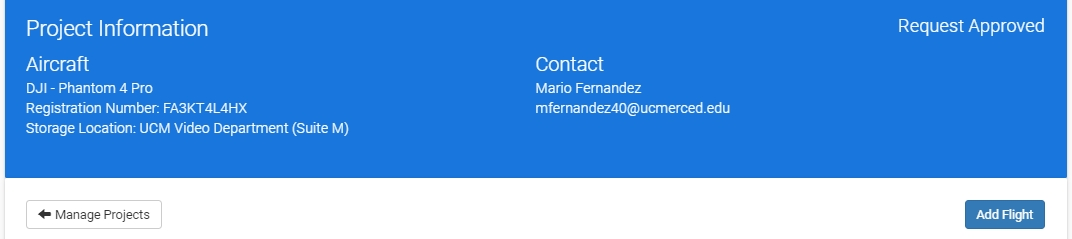
\includegraphics[width=0.85\linewidth]{images/UCDrones_project_addflight} 

}

\caption{UC Drones Project Management}\label{fig:UCDrones-project-flight-2}
\end{figure}

\hypertarget{submitting-a-flight-request}{%
\section{Submitting a Flight Request}\label{submitting-a-flight-request}}

An individual Flight Request comprises of one or more drone flights on a single day. Each Flight Request is reviewed individually, typically to address local issues such as campus safety, scheduling or privacy concerns.

\textbf{Example Individual Flight Requests}

\begin{itemize}
\tightlist
\item
  Any site that the field manager requires prior approval for scheduling or wildlife considerations
\item
  Athletic or recreational fields that require scheduling
\item
  On-campus public areas without additional mitigation protocols or safety hazard analysis.
\item
  Special operations -- flying at night, flying above 400 ft AGL, etc
\end{itemize}

\hypertarget{flight-request-form}{%
\subsection{Flight Request Form}\label{flight-request-form}}

The Flight Request form is nearly identical to the Project Request Form, except for 1 key difference. Whereas the Project Request form asks for a date range, frequency of occurrence and expected range of time, the Flight Request form requests a specific date and time.

When answering the specific date and time, be as specific as necessary. If the location is time sensitive, such as a field reservation, or in between a busy time on campus, please specify the exact time. But if the location does not have any time-related variation in safety, an approximate or estimate time is acceptable.

\begin{figure}

{\centering 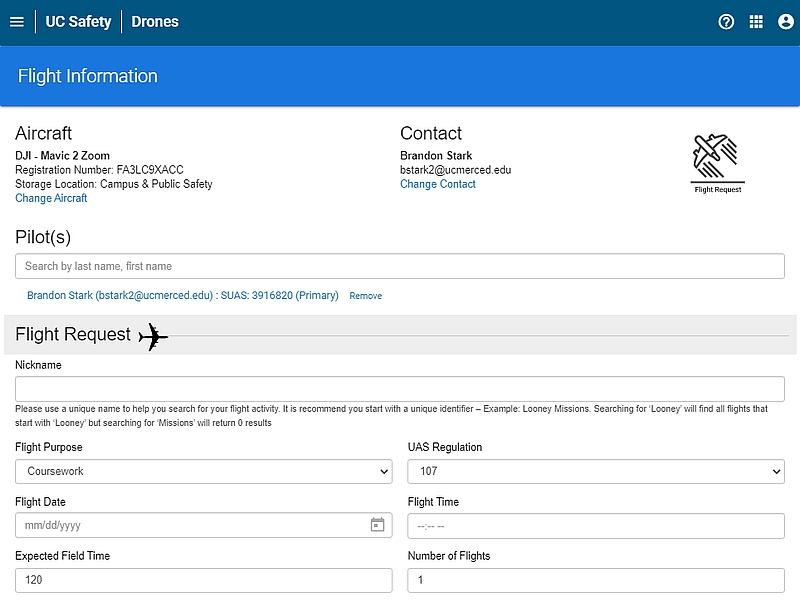
\includegraphics[width=0.85\linewidth]{images/UCDrones_flight_request} 

}

\caption{UC Drones Flight Request}\label{fig:UCDrones-flight-request}
\end{figure}

\hypertarget{non-project-vs-project-flight}{%
\subsection{Non-Project vs Project Flight}\label{non-project-vs-project-flight}}

Both Projects and Non-Projects use the same Flight Request Form. A Flight Request for a Project must be selected from the Project Page - either the Manage Projects Page and select `Add Flight' (Figure \ref{fig:UCDrones-project-flight-1}) or from the individual Project page and select `Add Flight' under the header (\ref{fig:UCDrones-project-flight-2}).

\begin{figure}

{\centering 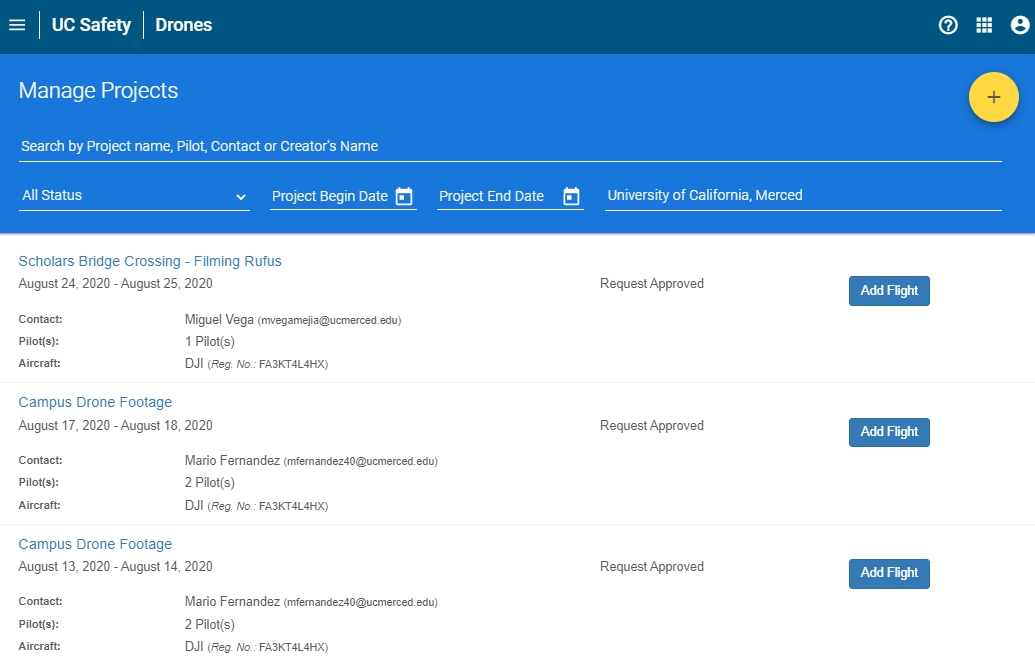
\includegraphics[width=0.85\linewidth]{images/UCDrones_manage_project} 

}

\caption{UC Drones Manage Projects}\label{fig:UCDrones-project-flight-1}
\end{figure}

\textbf{Differences}

\begin{itemize}
\tightlist
\item
  A Flight Request for a Project is automatically approved upon submission
\item
  A Flight Request for a Project is autofilled with the Project information

  \begin{itemize}
  \tightlist
  \item
    Only a handful of fields may be changed or completed
  \end{itemize}
\end{itemize}

\hypertarget{UCDrones-drone}{%
\section{Add your Drone to UC Drones}\label{UCDrones-drone}}

To register your drone with the UC system, add your drone to UC Drones.

\hypertarget{manag-aircraft}{%
\subsection{Manage Aircrafts}\label{manag-aircraft}}

The Manage Aircrafts page lists all the drones registered with your campus. From here, you can see the name, make/model, registration number as well as the Responsible Person for each drone.

\begin{itemize}
\tightlist
\item
  While you can see each drone at your campus, only the Responsible Person may edit the properties, or view the additional properties of the drone.
\end{itemize}

\begin{figure}

{\centering 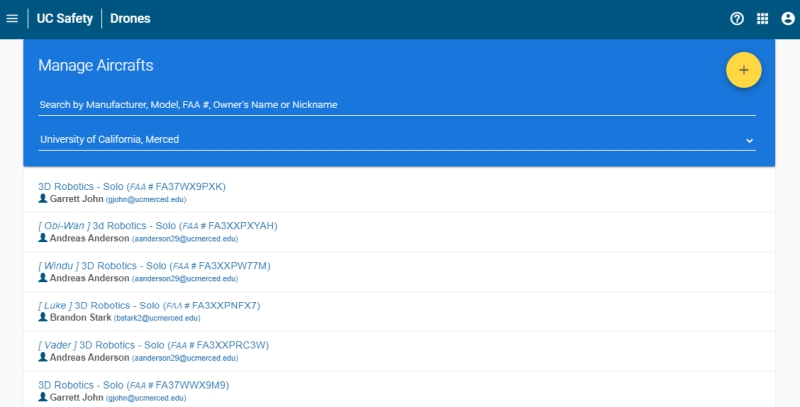
\includegraphics[width=0.95\linewidth]{images/UCDrones_manage_drones} 

}

\caption{UC Drones Manage Aircrafts}\label{fig:UCDrones-manage-aircrafts}
\end{figure}

\hypertarget{add-an-aircraft}{%
\subsection{Add an Aircraft}\label{add-an-aircraft}}

To add an aircraft to the list, click on the yellow + button in the upper right corner of the Manage Aircraft's page (Figure \ref{fig:UCDrones-manage-aircrafts})

On the Register an Aircraft Page, fill out the following information

\begin{figure}

{\centering 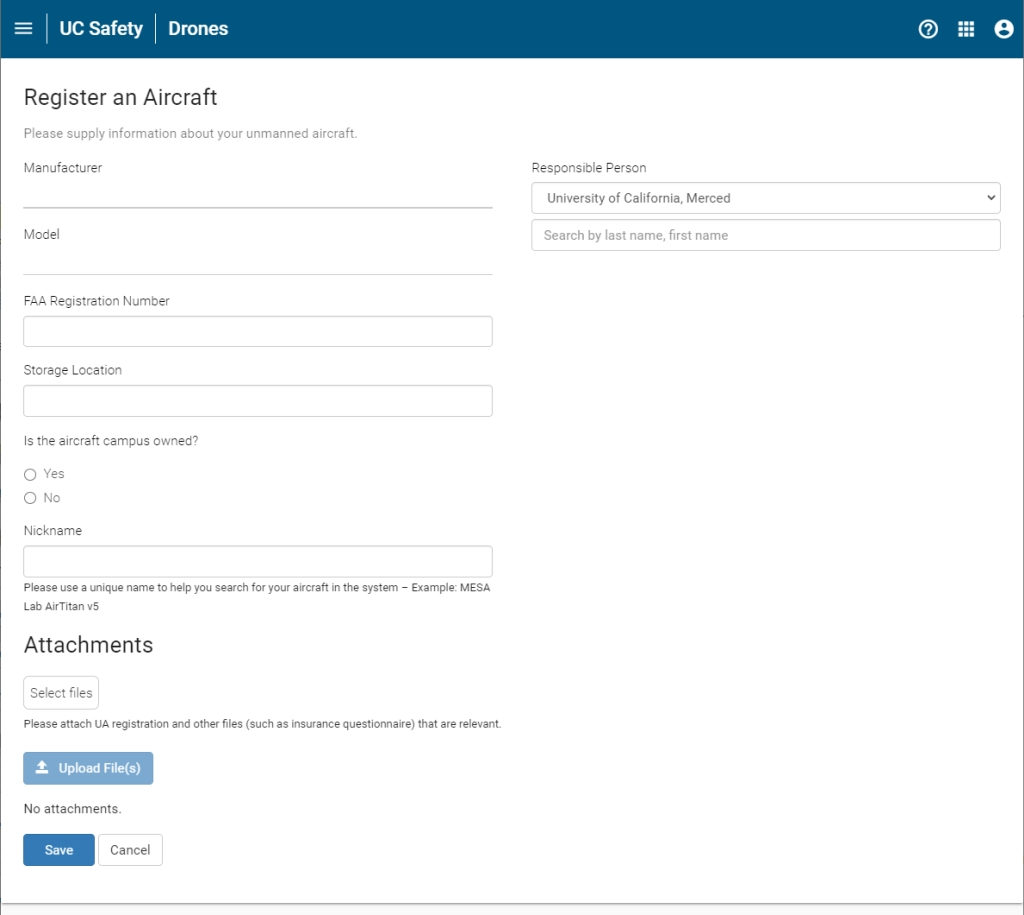
\includegraphics[width=0.95\linewidth]{images/UCDrones_aircraft} 

}

\caption{UC Drones Add/Edit Aircraft}\label{fig:UCDrones-edit-aircrafts}
\end{figure}

\begin{enumerate}
\def\labelenumi{\arabic{enumi}.}
\item
  \textbf{Responsible Person}

  Search the campus directory for the person who is designated responsible for the management and updating of the drone's information within UC Drones. This can be the regular pilot, administrative staff or PI. This can be changed or updated at any time.
\item
  \textbf{Manufacturer}

  Enter the manufacturer of your drone. If your drone is a kit build, use the name of the kit manufacturer. If your drone is a custom-build, you may enter `UC-Custom' or `Personal-Custom' whichever is appropriate.
\item
  \textbf{Model}

  Enter the model name of your drone. Please be sure to include any relevant suffixes (eg. Phantom 4 Pro V2)
\item
  \textbf{FAA Registration Number}

  All drones over 0.55 lbs and flown outside within the US must have an FAA registration number. This number is a 10 digit alphanumeric code that starts with FA. In some cases, it may also be an alphanumeric code that starts with N (N-number). If the drone will exclusively be flown indoors or is under 0.55 lbs, enter the serial number (or an identifying number for a custom build). There are special cases for drone flown exclusively outside of the US - please contact us at \href{mailto:UASsafety@ucmerced.edu}{\nolinkurl{UASsafety@ucmerced.edu}} for further instructions.
\item
  \textbf{Storage Location}

  Please enter the storage location of the aircraft, including building name and room number. If the aircraft is not used for University business, this question may be ommitted.
\item
  \textbf{Campus Owned}

  Please select whether the aircraft is owned by the University (ie, purchased with campus funds, research funds, educational funds) or is personally-owned.
\item
  \textbf{Nickname}

  Enter a short nickname for your drone. While your drone is searchable via the FAA registration number, you may also use a unique nickname to quickly find your drone while within the UC Drone web app. We recommend sticking to a common naming scheme such as PI-Model-Number
\item
  \textbf{Attachments}

  You may attach additional files, such as the FAA registration pdf or purchase invoice, for easy retrieval. Remember, for the UC UAS Replacement/Property insurance, we need to have a copy of the original purchase invoice so storing it here will make it easier to collect it.
\end{enumerate}

\hypertarget{safety}{%
\chapter{Drone Safety}\label{safety}}

Drone flight safety beings with planning - lots of things can go wrong, but if you're prepared, you can mitigate issues.

In this chapter, we'll go over a variety of safety tips, including some standard guidance, mission planning guidance and fire safety.

\begin{figure}

{\centering 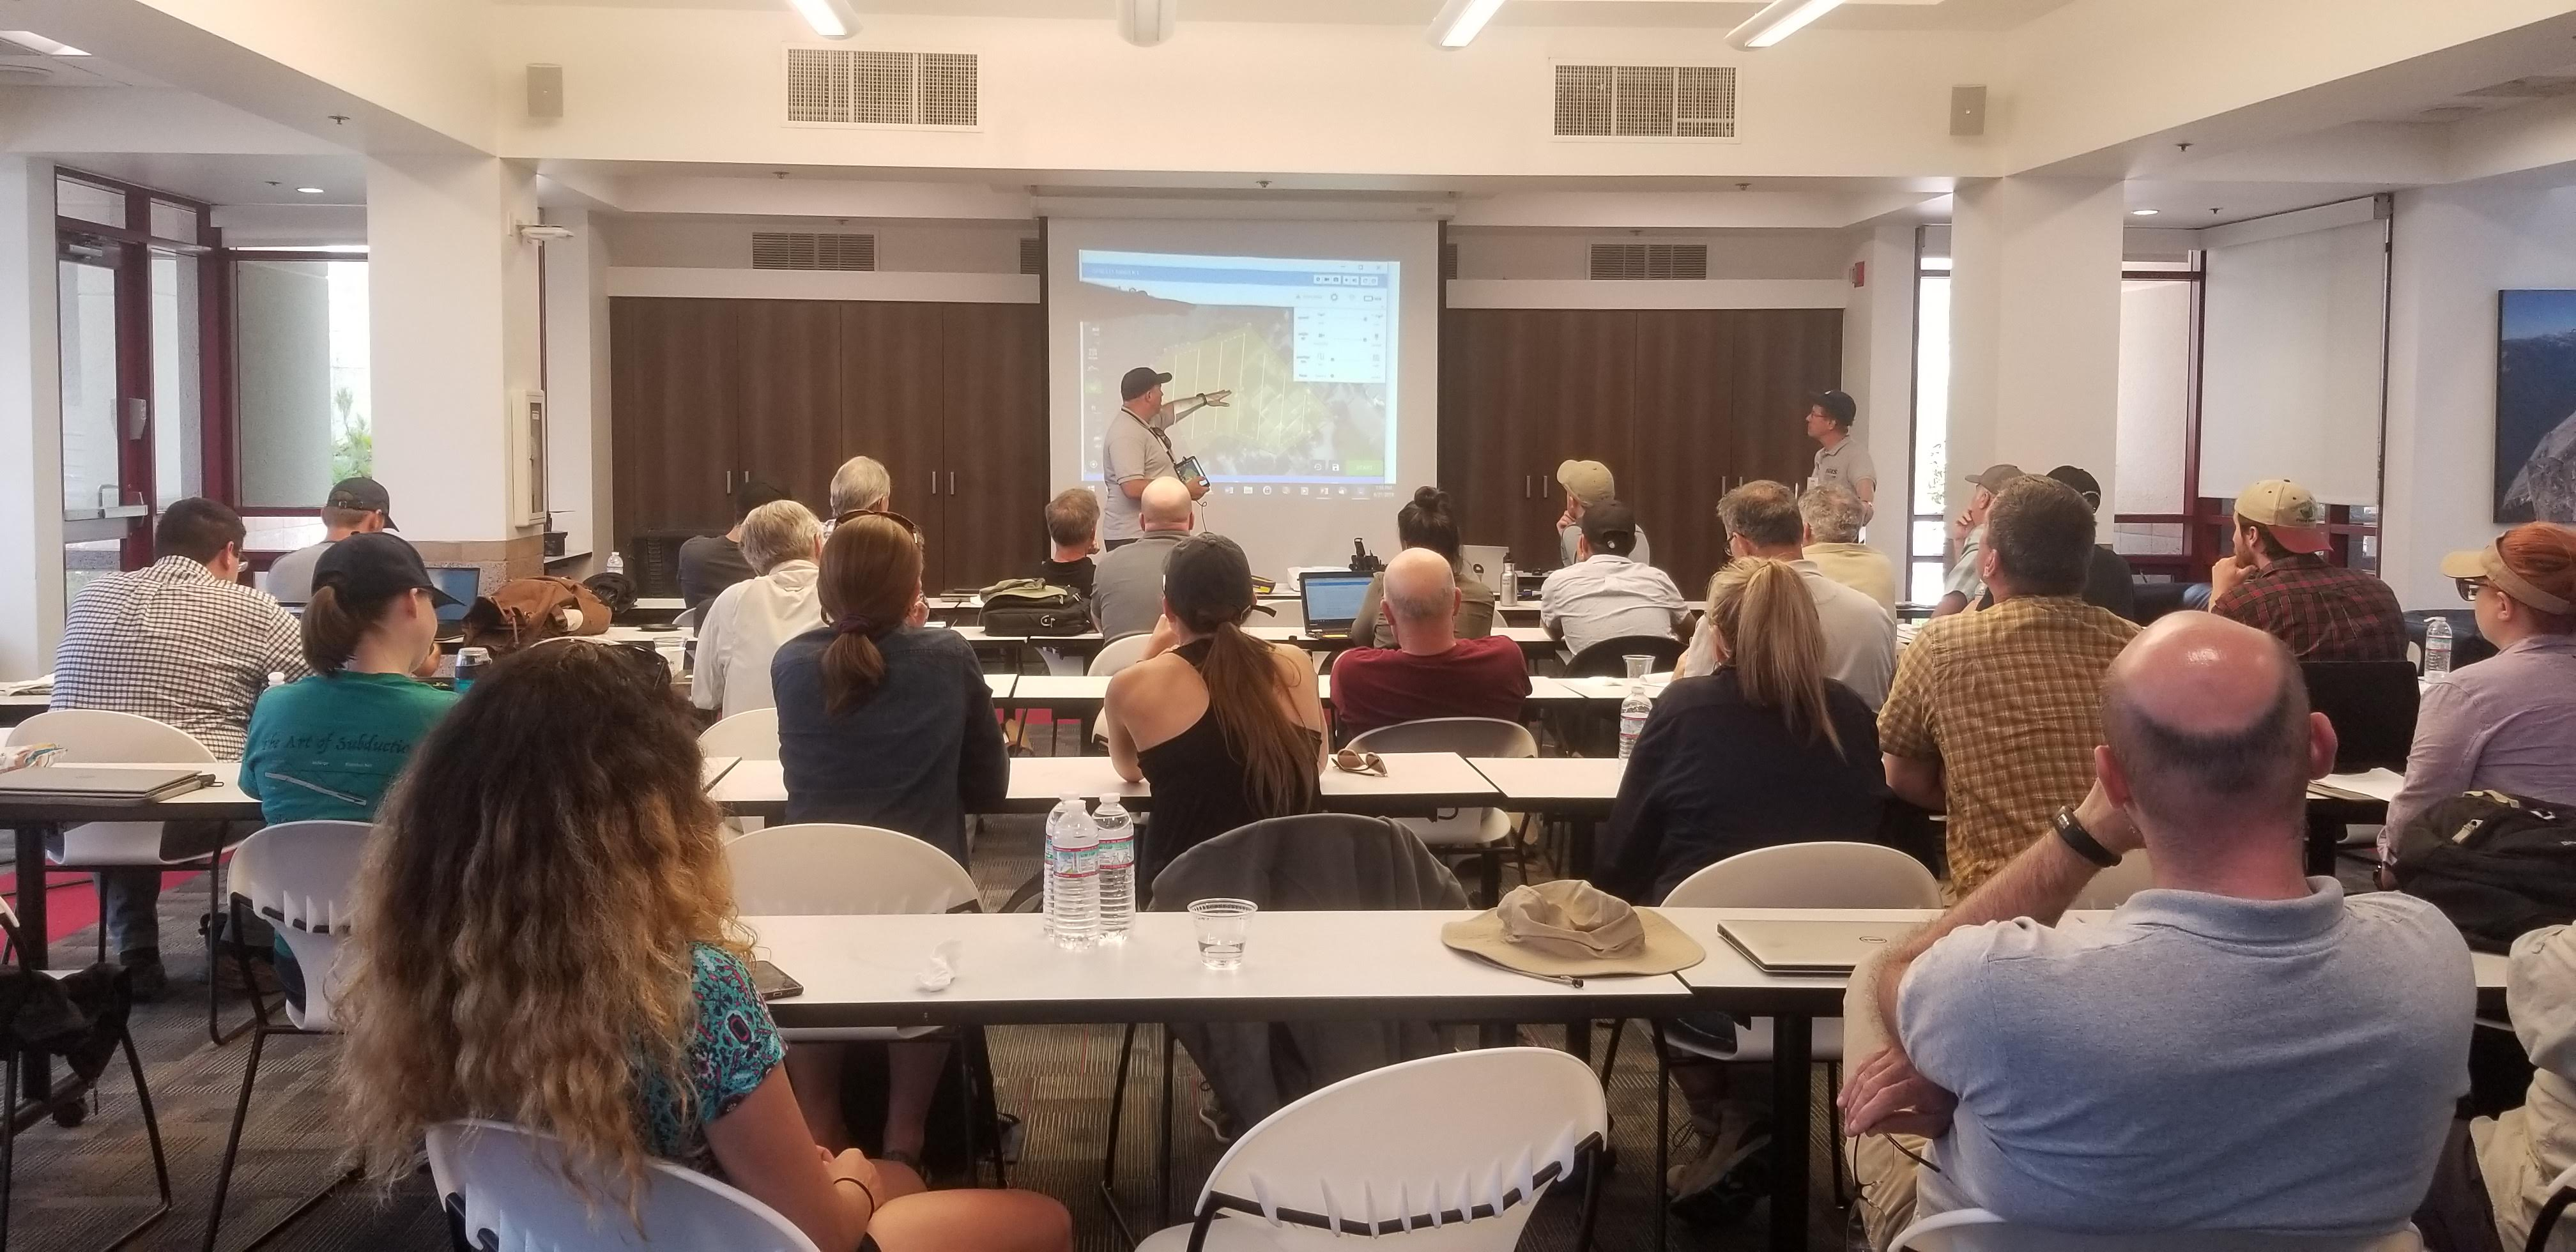
\includegraphics[width=0.75\linewidth]{images/training_1} 

}

\caption{DroneCamp Training Workshop}\label{fig:training}
\end{figure}

\hypertarget{drone-safety-standards}{%
\section{Drone Safety Standards}\label{drone-safety-standards}}

There's a lot of items to consider when it comes to drone safety. Here, we'll just give a couple of standard guidance:

\hypertarget{standard-guidance}{%
\subsection{Standard Guidance}\label{standard-guidance}}

\begin{itemize}
\tightlist
\item
  Establish a \textbf{buffer} or \textbf{safe-zone} between the Unmanned Aircraft and any non-participating persons or sensitive locations. A good rule-of-thumb is to maintain a buffer or safe-zone of \textbf{roughly \(\frac{1}{4}^{th}\) of the flight altitude}.
\item
  \textbf{Visual Observers} and supporting ground crew should be utilized when available. Supporting ground crew should assist in ensuring safety to all non-participating persons.
\item
  All members of the flight crew should \textbf{be conspicuous} and wear \textbf{professional, identifying apparel} such as university-branded hats, shirts or lanyards with IDs.
\item
  \textbf{High visibility reflective vests} must be worn when operating \textbf{near roads} or \textbf{in parking lots}.\\
\item
  When operating in fenced areas, \textbf{stay within the fenced areas} unless there is sufficient visibility on the other side to ensure safety to non-participants.
\item
  Never fly in areas where \textbf{drone activity is prohibited or restricted}.
\item
  \textbf{Always be a good neighbor} and ensure that your drone activity is not disruptive to other authorized activities.
\item
  Pay attention to \textbf{sloping terrain and trees}. It is too easy to misjudge and autonomously fly into a tree.
\end{itemize}

\begin{figure}

{\centering 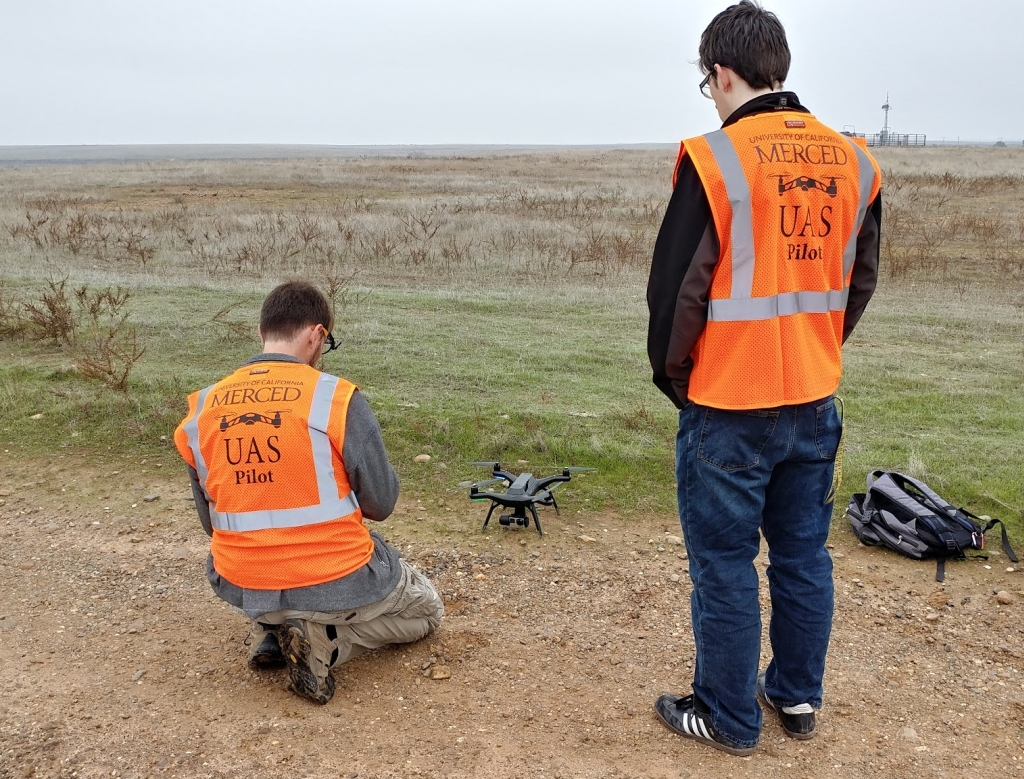
\includegraphics[width=0.75\linewidth]{images/UAS_vest} 

}

\caption{UAS operators with high visiblity vests, UC Merced}\label{fig:hivis}
\end{figure}

\hypertarget{operating-on-campus-or-other-busy-locations}{%
\subsection{Operating on Campus or other busy locations}\label{operating-on-campus-or-other-busy-locations}}

\begin{itemize}
\tightlist
\item
  Utilize the \textbf{UC UAS Mission Planning Template} (\href{http://ucdrones.github.io/library/mission_planning_template.docx}{link}) to systematically develop your flight plan
\item
  \textbf{Pre-plan each flight} in detail when operating in \textbf{uncontrolled locations} in proximity to non-participating person. Use this planning to look for potential safety issues and identify mitigating actions.
\item
  \textbf{High visibility vests are recommended} when near nonparticipants or in public areas.
\item
  Don't rely on passive crowd control measures such as \textbf{Orange cones}. Supplement any portable pedestrian control equipment (cones, caution tape, signs) with ground personnel. If spectators are expected, a supporting ground crew member should be tasked with \textbf{preventing spectators from distracting the RPIC} with questions or comments.
\item
  When operating near roads, a supporting ground crew member should be tasked with being located near the road to monitor traffic, and if necessary, retrieve a fallen Unmanned Aircraft before it becomes a road hazard.
\item
  \textbf{Flying above buildings and structures may minimize risk} to pedestrians, but contact the facility manager to properly evaluate the potential risks. Some \textbf{campus buildings are outfitted with research or communication equipment} on rooftops.
\end{itemize}

\hypertarget{mission}{%
\section{Planning a Mission}\label{mission}}

Plan your flight mission with safety in mind from the get go. Use the Site Analysis process to figure out exactly how to accomplish your mission and determine any other supplies or support you might need.

\hypertarget{site-analysis-process}{%
\subsection{Site Analysis Process}\label{site-analysis-process}}

One of the best things you can do when you start planning your mission is to conduct a thorough site analysis process. Do a methodical review of where you want to fly, taking into consideration what you want out of the flight and any hazards that exist.

Following your methodical review, you can start planning your flight paths, assess visibility, decided where to put VOs or other helpers, and have ample details for any emergency action plans.

\hypertarget{site-analysis-steps}{%
\subsection{Site Analysis Steps}\label{site-analysis-steps}}

\begin{itemize}
\tightlist
\item
  Print out a satellite image of the site
\item
  Evaluate Data Requirements

  \begin{itemize}
  \tightlist
  \item
    Identify the region(s) of interest
  \item
    Identify the best visual angles

    \begin{itemize}
    \tightlist
    \item
      Consider the time of day, shadows and reflective surfaces
    \end{itemize}
  \item
    Estimate the best flight region and flight paths
  \end{itemize}
\item
  Identify any constraints

  \begin{itemize}
  \tightlist
  \item
    Mark any airspace issues

    \begin{itemize}
    \tightlist
    \item
      Airspace Class
    \item
      Airports, Heliports
    \item
      Flight Patterns
    \end{itemize}
  \item
    Mark any vertical structures

    \begin{itemize}
    \tightlist
    \item
      Changes in elevation
    \item
      Buildings
    \item
      Towers, powerlines
    \item
      Trees
    \item
      Other vertical obstructions
    \end{itemize}
  \item
    Mark any ground obstructions

    \begin{itemize}
    \tightlist
    \item
      Smaller structures
    \item
      Gates, Fences
    \item
      Hedges, Shrubs
    \item
      Other obstructions that may impede access
    \end{itemize}
  \item
    Identify any other safety or regulatory issue

    \begin{itemize}
    \tightlist
    \item
      Fire risks
    \item
      Wildlife impacts
    \item
      Physical access to site
    \end{itemize}
  \item
    Identify potential site access points by non-participants

    \begin{itemize}
    \tightlist
    \item
      Pedestrian walkways
    \item
      Bike paths
    \item
      Building doors/access points
    \end{itemize}
  \end{itemize}
\item
  Refine flight plan with constraints

  \begin{itemize}
  \tightlist
  \item
    Select a launch/recovery site that can be reasonably secured
  \item
    Assess whether any vertical structure may impede visual line of sight
  \item
    Assess whether any ground obstruction may limit any emergency recovery operations
  \item
    Consider multiple flights per Mission to achieve mission goals
  \end{itemize}
\item
  Plan flight crew locations

  \begin{itemize}
  \tightlist
  \item
    Pilot and VO at Launch/Recovery point

    \begin{itemize}
    \tightlist
    \item
      Consider if Pilot/VO may require relocation during flight operation
    \end{itemize}
  \item
    Remote VOs and other ground crew support

    \begin{itemize}
    \tightlist
    \item
      May be tasked to redirect non-participant traffic away from flight zone
    \end{itemize}
  \end{itemize}
\item
  Iterate as necessary to meet Mission Objectives
\end{itemize}

\hypertarget{site-analysis-guide}{%
\subsection{Site Analysis Guide}\label{site-analysis-guide}}

Please visit the webpage for a walkthrough of the Site Analysis Process

\hypertarget{resources}{%
\subsection{Resources}\label{resources}}

Make regular use of planning tools and resources here: \href{https://ucdrones.github.io/ch-resources.html}{UC Drones Resources}. Don't be afraid to edit/update/modify them as you see fit. All of these should be considered living documents, tailored to enable you to make safety decisions with as much information as possible.

\hypertarget{fire-safety}{%
\section{Fire Safety}\label{fire-safety}}

While UAS accidents and incidents involving fire are rare, they are a valid and significant concern. With the majority of UC UAS usage on field sites and other rural locations, the potential for the accidental sparking of fire is a concern. A fire sparked by a UAS can spread quickly (Figure \ref{fig:fire-start}) and with California's dry environment, can cause significant damage (Figure \ref{fig:fire-damage}).

Everyone who flies a drone within the UC should take the \href{https://ucdrones.github.io/library/trainings/FireSafety/index.html}{Drone Fire Safety Training Course}

\begin{figure}

{\centering 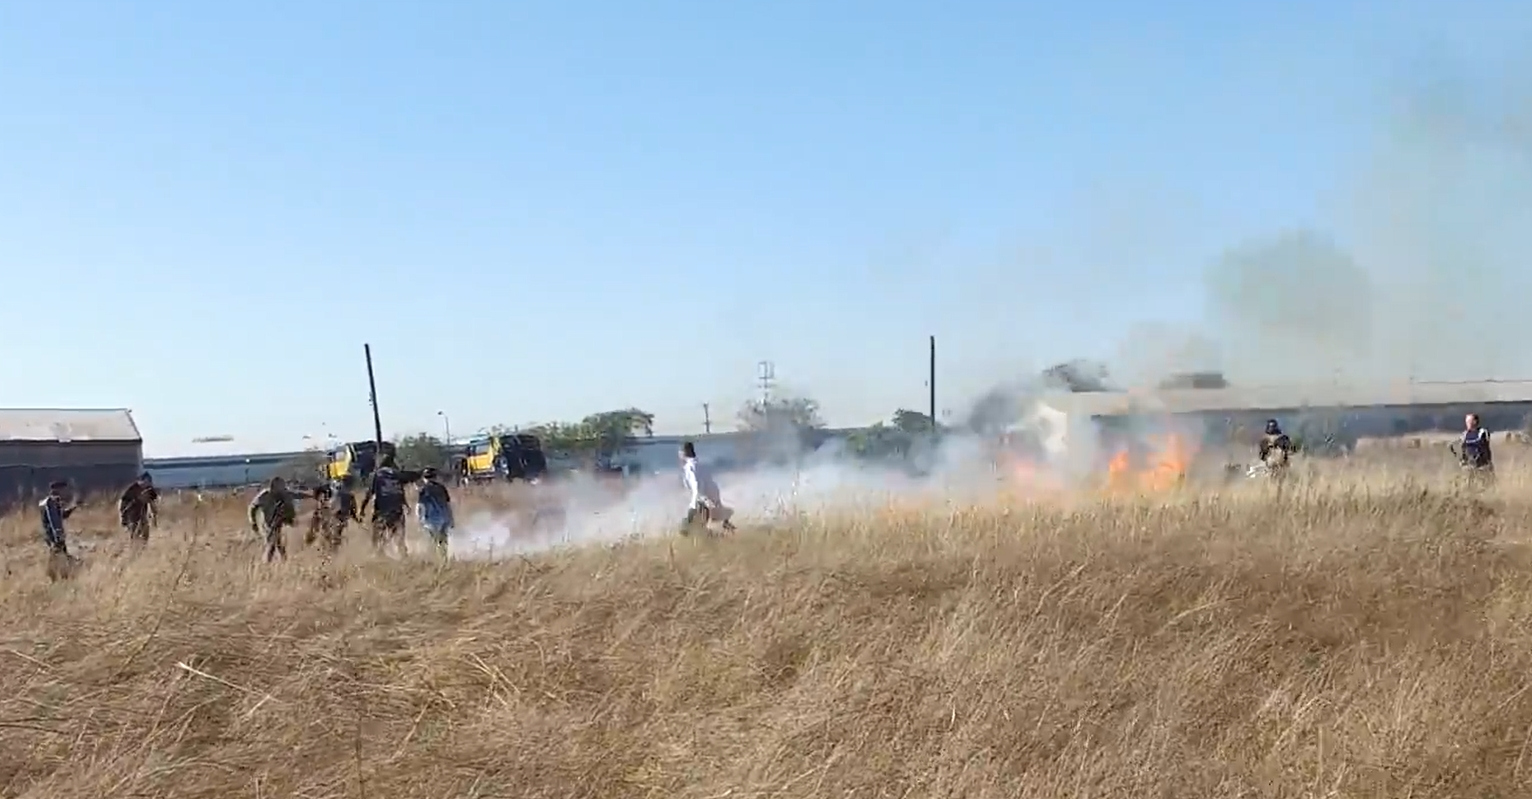
\includegraphics[width=0.75\linewidth]{images/fire_start} 

}

\caption{Beginning of a fire from UAS accident at Richmond Field Station, UC Berkeley}\label{fig:fire-start}
\end{figure}

\begin{figure}

{\centering 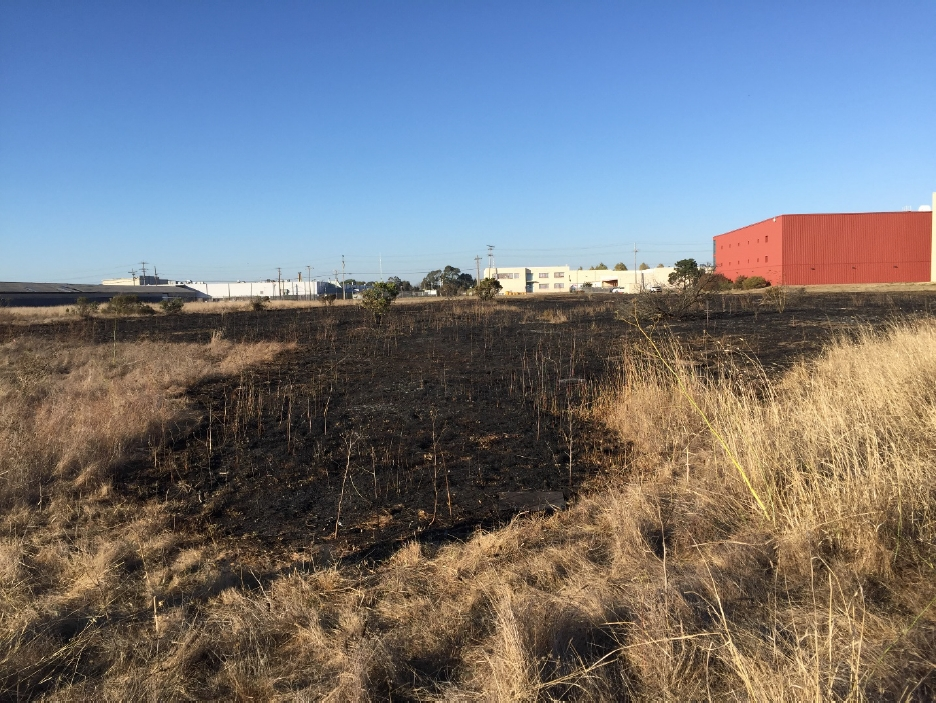
\includegraphics[width=0.75\linewidth]{images/fire_damage} 

}

\caption{Post fire damage from UAS accident at Richmond Field Station, UC Berkeley}\label{fig:fire-damage}
\end{figure}

\hypertarget{lipo-battery-guidance}{%
\subsection{LiPo Battery Guidance}\label{lipo-battery-guidance}}

The most common cause of drone related fire is from misuse of LiPo batteries. Special care should be taken when charging, discharging or storing LiPo batteries. If the internal polymer cell of a LiPo battery is exposed to air, a violent chemical reaction starts that could explode, but more commonly releases significant amounts of smoke and heat that can ignite other fire fuel sources. A LiPo battery fire is typically caused by a physical puncture to the battery or from misuse, such as overcharging or electrical shorts.

\textbf{Recommended Best Practices}

\begin{itemize}
\item
  Always thoroughly inspect a battery before charging and use.

  \begin{itemize}
  \tightlist
  \item
    Look for swelling, puffy cells, cracks in plastic, and charred debris along the contacts.
  \end{itemize}
\item
  Never use a battery that is not in good health.

  \begin{itemize}
  \tightlist
  \item
    Consider batteries to be replaceable and consumable, rather than a permanent component of the UAS.
  \end{itemize}
\item
  Never store batteries in a hot car.
\item
  Don't charge your batteries unless you're going to fly within the next day.
\item
  After immediate use, place battery out of the sun but do not place within a closed container.

  \begin{itemize}
  \tightlist
  \item
    Ensure there is sufficient airflow to allow the battery to cool.
  \end{itemize}
\item
  When done flying for the day, always charge your batteries at least back up to storage level.
\item
  Do not charge an intelligent flight battery immediately after flight as the temperature may be too high. Wait until it cools down to room temperature before charging again.
\item
  Store the battery in a dry and cool place, keep out of direct sunlight and away from any liquids
\item
  Do not store or transport a battery with eyeglasses, watches, metal necklaces or other metal components that may short the battery
\item
  When in transport, store the batteries in a safe container that will protect it from damage, squeezing, puncturing or falling.
\end{itemize}

\hypertarget{planning-for-fire-mitigation}{%
\subsection{Planning for Fire Mitigation}\label{planning-for-fire-mitigation}}

In addition to LiPo battery care, special effort must be taken to consider the fire risks in drone activity. Consult the appropriate department (Fire, Field Safety, EH\&S) if there are concerns over fire risk. Minimize the potential for fire by monitoring where the drone will be flying and ensure that if a fire was to occur, the RPIC and any other persons, such as Visual Observers, are prepared to respond appropriately.

\textbf{Guidance for fire safety}

\begin{itemize}
\item
  Everyone should take the \href{https://ucdrones.github.io/library/trainings/FireSafety/index.html}{drone fire safety training course}
\item
  Avoid flying on high fire risk days, including \href{https://www.fire.ca.gov/programs/communications/red-flag-warnings-fire-weather-watches/}{Red Flag Warning} alerts issued by CAL FIRE.
\item
  Never fly alone in areas of moderate to high fire risk
\item
  Always bring a fire extinguisher and a shovel/bucket of sand to field sites.
\item
  During flight operations:

  \begin{itemize}
  \tightlist
  \item
    Ensure that a crew member has easy access to fire equipment.
  \item
    Ensure that a crew member has easy access to reach any location where the drone may crash.
  \item
    Ensure that a crew member has the ability to report an emergency situation and can adequately provide directions for emergency personnel to reach the site.
  \end{itemize}
\item
  When flying in high fire risk locations, use high quality, commercially available drones with enclosed electronics.
\item
  Never fly a damaged or swollen battery.
\end{itemize}

\hypertarget{drone-fire-safety-bucket}{%
\subsection{Drone Fire Safety Bucket}\label{drone-fire-safety-bucket}}

Come prepared for a fire by packing this Drone Fire Safety Bucket, designed by \textbf{Victor Duraj} at \textbf{UC Davis}. It is based around a 7-gallon red bucket in order to accommodate a larger extinguisher, to help the bucket physically stand out on a flight site, and to reference it efficiently in an emergency as ``that red fire bucket''. It includes a screw top lid, a fire extinguisher, a fire blanket, a folding camp shovel, a fluorescent orange flag, a first aid kit, a storage clipboard, self-made labels, and a double-sided laminated Contents \& Instructions sheet.

\begin{figure}

{\centering 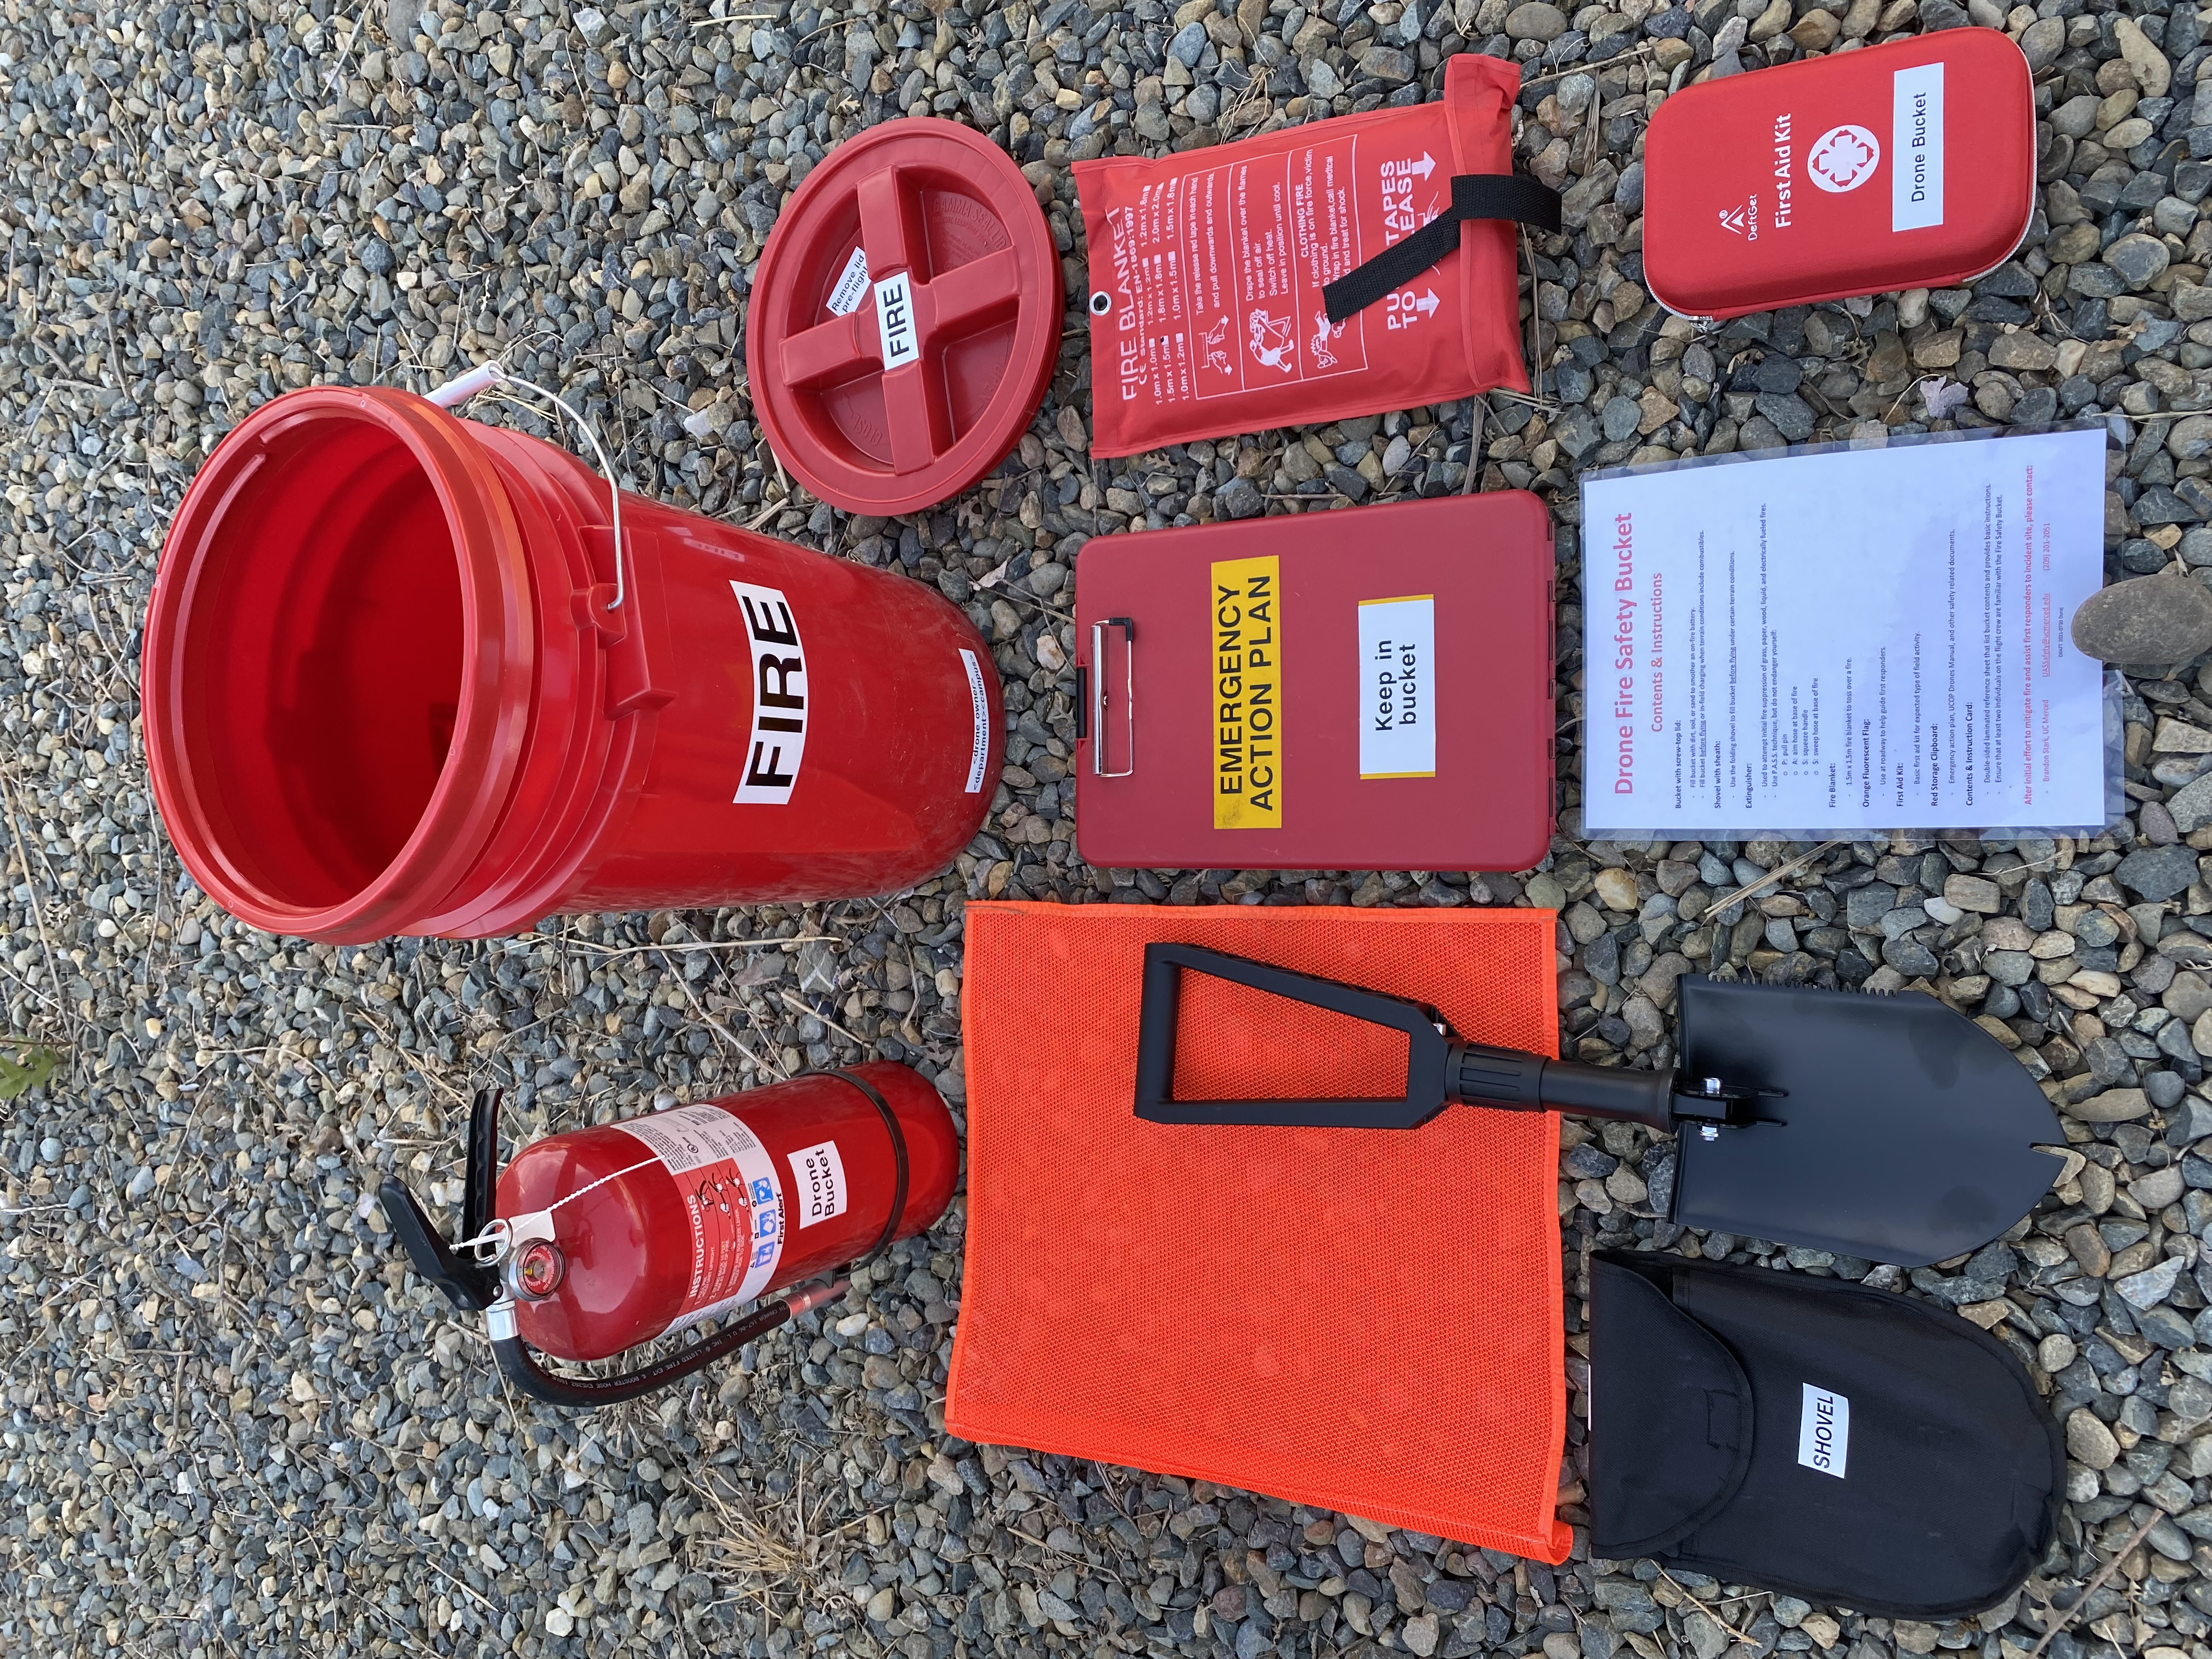
\includegraphics[width=0.75\linewidth]{images/DroneFireBucket} 

}

\caption{Drone Fire Bucket}\label{fig:fire-bucket}
\end{figure}

\href{https://ucdrones.github.io/library/drone_fire_safety_bucket.docx}{Contents \& Instruction Sheet}

\hypertarget{tips}{%
\section{Top 10 Safety Tips}\label{tips}}

Good pilots aren't born, they are forged with training, practice and experience. When starting on your drone journey, follow these 10 tips for being a safe pilot.

\begin{enumerate}
\def\labelenumi{\arabic{enumi}.}
\tightlist
\item
  \textbf{Practice} - There is no substitute for experience. Gain experience by practicing flying your drone, conducting data collection missions, and flight planning. Get familiar with your equipment and processes.
\item
  \textbf{Write Everything Down} - Keeping records can help you maintain your equipment, monitor for unsafe practices and keep you on track. Things to track: battery usage, weather conditions, equipment use/damage, software versions.
\item
  \textbf{Make Checklists and Use Them} - Nothing derails a flight mission like forgetting an item or a step. Make a checklist for planning a mission, make a checklist for packing your equipment, make a checklist for preflight inspections and any other process you may have.
\item
  \textbf{Always Keep an Eye on the Weather} - Experienced field researchers know that weather reports are only a suggestion. Conditions in the field may change dramatically and can turn a good flying day to a disaster.
\item
  \textbf{Bring a friend or two} - Between juggling a flight controller, operating a payload, monitoring weather conditions and scanning for intruding air traffic, it can be taxing to try to do it all at an appropriate level. Bring some help to make sure everything goes smoothly.
\item
  \textbf{Bring backups or replacement parts} - Many operators will bring spare propellers or batteries to their flight missions, but don't forget about other supporting equipment such as cables, landing gear, radios or antennas. Make sure backup parts are on your pre-departure checklist.
\item
  \textbf{Choose appropriate flight locations} - When you choose a location to fly at, make sure you're aware of all the hazards. Look for indicators of hidden hazards like rolling hills or high tree lines that create turbulence, or low visibility hazards such as power-lines or towers that interfere with radio systems. Be aware that you as the pilot are responsible of ensuring the safety of all persons on the ground, whether you can see them or not.
\item
  \textbf{Set boundaries for go/no-go situations and stick to them} - Deciding when to fly and when not to fly should not be an ambiguous decision. Don't let external pressures push you to make unsafe decisions.
\item
  \textbf{If something isn't right, stop immediately} - Nothing fixes itself in the air. If something doesn't sound right on the ground during pre-flight checks, don't fly. If the weather changes to an unsafe condition, land as soon as it is safe.
\item
  \textbf{Pause and consider all the risks before you fly} - Damage to your aircraft is only one of many aspects to consider. Consider the payload, consider potential damage to other's property, consider secondary effects such as causing an auto accident when your aircraft crashes in the middle of a road.
\end{enumerate}

\hypertarget{ch-privacy}{%
\chapter{Drones and Privacy}\label{ch-privacy}}

The capture and use of photographs and videos from a drone raises new concerns on the rights, privacies, and permissions that involve both the operators of a drone and individuals that are uninvolved in the operation.

The University of California recognizes the important value of privacy and strives to achieve an appropriate balance ensuring an appropriate level of privacy, nurturing an environment of openness, honoring its obligation as a public institution to remain transparent while safe guarding information about individuals.

\begin{figure}

{\centering 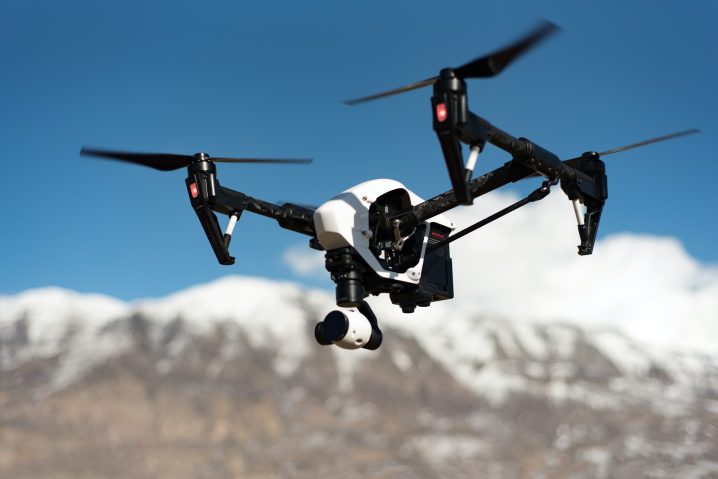
\includegraphics[width=0.75\linewidth]{images/inspire_1} 

}

\caption{Flying Cameras}\label{fig:drone1}
\end{figure}

\hypertarget{best-practices}{%
\section{Best Practices}\label{best-practices}}

\begin{itemize}
\item
  \textbf{Do not} use a drone to monitor or record activities where there is a reasonable expectation of privacy.
\item
  \textbf{Do not} use a drone for unapproved recordings of any campus events or performances, or for any unlawful purposes.
\item
  \textbf{Do not} use a drone to harass people or intentionally disrupt events.
\item
  \textbf{Do not} fly a drone over private property without prior approval.
\item
  \textbf{Do not} use a drone for the specific purpose of persistent and continuous collection of identifiable data about individuals without the consent of the data subjects.
\item
  \textbf{Do not} retain identifiable data longer than reasonably necessary to fulfill a purpose.
\item
  \textbf{Do not} knowingly publicly disclose data collected with a drone without undertaking a reasonable effort to obfuscate or de-identify identifiable data unless the data subjects provide specific consent to the disclosure.
\item
  \textbf{Do} make a reasonable effort to remain conspicuous and visible during flight operations.
\item
  \textbf{Do} make a reasonable effort to provide prior notice to individuals of the general timeframe and area that they may anticipate a drone intentionally collecting data.
\item
  \textbf{Do} establish and make available a Privacy Statement for drone data if the drone may intentionally or unintentionally collected identifiable data. The policy should be appropriate to the size and complexity of the data collected.
\item
  \textbf{Do} be considerate of other people's concerns over privacy, security and safety.
\item
  \textbf{Do} contact the Office of Research Compliance and Integrity if identifiable data is to be used for human-subject research.
\item
  \textbf{Do} take steps to ensure the security of any identifiable data.
\end{itemize}

\hypertarget{privacy-statement}{%
\section{Privacy Statement}\label{privacy-statement}}

An effective privacy statement is concise and easy to understand. Consult with your campus Privacy Officer or Institutional Review Board for additional help or guidance in developing an effective privacy policy.

\hypertarget{topics-for-a-privacy-statement}{%
\subsection{Topics for a Privacy Statement}\label{topics-for-a-privacy-statement}}

\begin{itemize}
\tightlist
\item
  The purposes for which the drone will collect identifiable data
\item
  The kinds of identifiable data the drone will collect
\item
  Information regarding any data retention and de-identification practices
\item
  Examples of the types of any entities with who identifiable data will be shared
\item
  Information on how to submit privacy and security complaints or concerns
\item
  Information describing practices in responding to law enforcement requests
\end{itemize}

NOAA has an excellent example of a detailed drone privacy statement: \protect\hyperlink{https:ux2fux2fwww.cio.noaa.govux2fitmanagementux2fpdfsux2fSigned_UAS_PrivacyPolicy.pdf}{Link, pdf}

\hypertarget{do-i-need-to-write-a-privacy-statement}{%
\subsection{Do I need to write a Privacy Statement}\label{do-i-need-to-write-a-privacy-statement}}

While most flight operations are on UC property and within dedicated research locations, such as field stations and reserves, a significant number of projects are on public land, near non-participants or in collaboration with private collaborators. As such, there may be unintentional impacts to the privacy and well-being of others. When in doubt, always consider putting together at least a minimal document.

\hypertarget{insurance}{%
\chapter{Drone Insurance}\label{insurance}}

Are you worried about crashing your drone? While we take a lot of steps to help you fly safely, accidents can happen. That's what insurance is for.

The UC provides comprehensive insurance coverage \textbf{free of charge} for drone operations. This includes both liability insurance coverage and replacement insurance.

\begin{itemize}
\tightlist
\item
  \textbf{Liability insurance} will cover the costs of any damage caused by a drone to another person or property. If your drone crashes and breaks a window, this is what liability insurance is for.
\item
  \textbf{Replacement insurance} will cover the costs of replacing or repairing a damaged, destroyed or lost drone. It has a deductible of \$1000. If your drone crashes into a tree and requires \$4,000 in repairs, you will be reimbursed the actual cost of repair, minus the deductible, for a total of \$3,000.
\end{itemize}

\hypertarget{liability-insurance}{%
\section{UC UAS Liability Insurance}\label{liability-insurance}}

The University of California has purchased an Unmanned Aircraft System Liability Policy. This policy has a total of \$5 Mil limit including Personal Injury.

Coverage is automatic for UAS activity that meet the following criteria:

\begin{itemize}
\tightlist
\item
  Flight operations are conducted on behalf and sanctioned by the University of California.
\item
  Aircraft weight under 55 lbs (at time of takeoff)
\item
  Flight operations are within Visual Line of Sight
\item
  Flight operations are below 400 ft above ground level.
\item
  Flight operations must be conducted within the United States.
\end{itemize}

Any UAS activity that do not meet the above criteria or operate outside the above criteria must be reported to and approved by the insurance underwriter in order to be covered.

\begin{notebox}
We will follow up with you if your flight operation is not automatically covered and will work with you to ensure coverage.

On rare occasions, typically on international UAS activity, you or your department may be required to purchase additional coverage.

\end{notebox}

Any UAS activity that is not approved by a Designated Local Authority or Systemwide Designated UAS Authority is not covered by this liability insurance coverage.

We recommend the use of UC Drones web app to ensure coverage - but please remember that if the Flight is not in the system as ``Approved'' you are not covered.

\begin{itemize}
\tightlist
\item
  An approved Project does not grant insurance coverage, you must submit a Flight notification or request to ensure insurance coverage.
\end{itemize}

\hypertarget{personally-owned-unmanned-aircraft-used-for-university-business}{%
\subsection{Personally Owned Unmanned Aircraft Used for University Business}\label{personally-owned-unmanned-aircraft-used-for-university-business}}

The University of California has extended their UAS liability policy to enable coverage of UAS owned by UC students, staff or faculty used for University Business, including research. Coverage in contingent on compliance with the policy and procedures on UAS usage. This coverage is not intended to cover student organizations or 3rd Party vendors or contractors.

\hypertarget{coverage-for-campus-police}{%
\subsection{Coverage for Campus Police}\label{coverage-for-campus-police}}

The University of California has extended their UAS liability policy to enable coverage of UAS by Campus Police. All coverage is contingent on the UAS activity being sanctioned by the UC.

Any UAS activity that is not approved by a Designated Local Authority or Systemwide Designated UAS Authority is not covered by this liability insurance.

\hypertarget{hull-insurance}{%
\section{UC UAS Replacement Insurance}\label{hull-insurance}}

Physical damage to a UAS is covered under a blanket policy issued by the University's captive insurance company, Fiat Lux Risk and Insurance Company

\begin{itemize}
\tightlist
\item
  Coverage applies in flight only when an approved flight plan is filed in accordance with UC UAS Policy, including the UC Drone web app or other means of compliance.\\
\item
  Coverage is limited to \$25,000 for Unmanned Aircrafts
\item
  Payload is covered separately and not included within this limit
\item
  \$1,000 deductible applies to each and every loss (including payload)
\item
  Coverage additionally applies in the event of theft, vandalism, fire and other perils in accordance to the UC Property Insurance Program.
\item
  In the event of a loss, please report to campus risk management.
\end{itemize}

This physical damage coverage does not extend to personally owned-UAS used for University Business. \textbf{Only UAS owned by the University of California are covered.}

\hypertarget{filing-a-claim}{%
\subsection{Filing a Claim}\label{filing-a-claim}}

To file a claim, contact your campus Risk Manager. Please prepare the following:

\begin{itemize}
\tightlist
\item
  Copy of the post-flight report (through UC Drones or other means of compliance)
\item
  Photographs of damaged equipment
\item
  Copy of original purchase invoice
\item
  Copy of invoice to ship the equipment back the manufacturer
\item
  Copy of repair invoice, if repairable
\item
  Copy of replacement quote, if not repairable
\end{itemize}

\textbf{Ensure your coverage}

\begin{itemize}
\tightlist
\item
  Attach a copy of your UAS invoice to your UAS registration in UC Drones
\item
  Make sure you file your Flight Requests
\item
  For recurrent or on-going activity, create a Project application but don't forget to add flights before you head out.
\item
  After an incident, make sure you take pictures of the damage and file a post-flight report. Add as much details as possible.
\end{itemize}

\hypertarget{drones-and-other-equipment}{%
\chapter{Drones and Other Equipment}\label{drones-and-other-equipment}}

\begin{figure}

{\centering 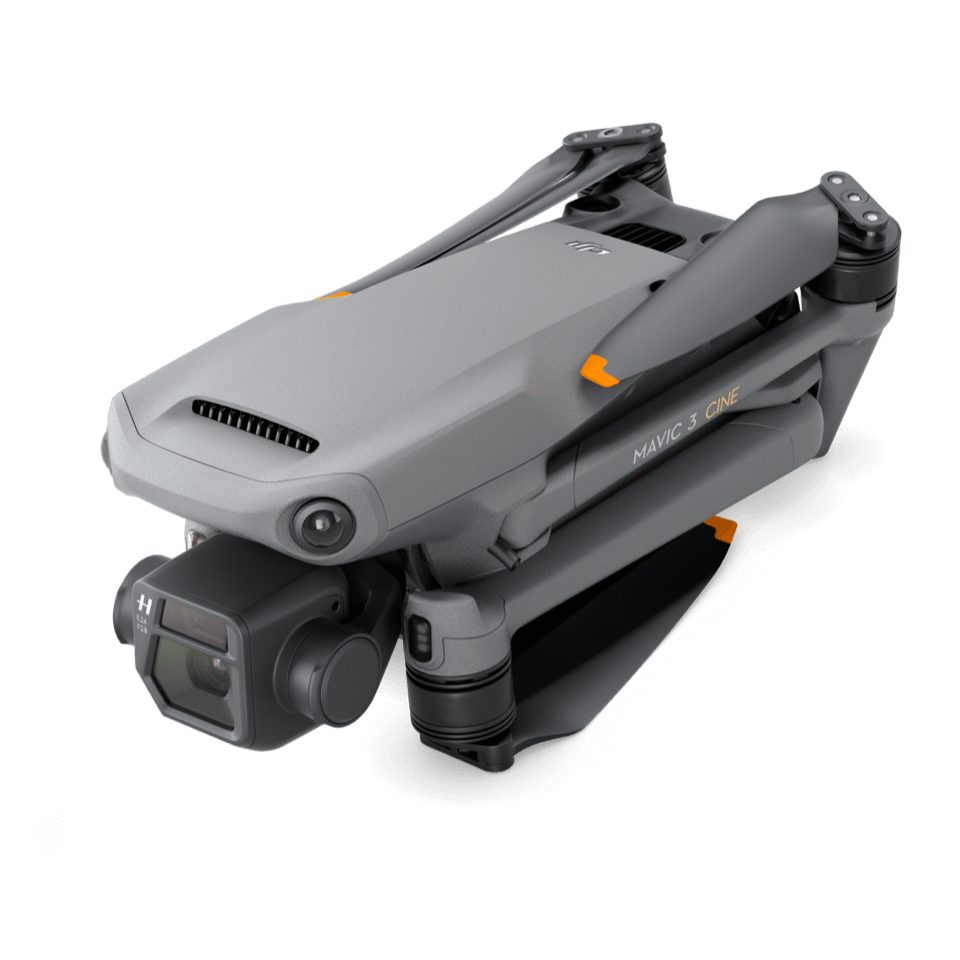
\includegraphics[width=0.75\linewidth]{images/mavic3} 

}

\caption{The Mavic 3 is the newest model, but is it the best drone for you?}\label{fig:drone3}
\end{figure}

\hypertarget{what-drone-should-be-get}{%
\section{What Drone should be get?}\label{what-drone-should-be-get}}

\hypertarget{essential-supplemental-drone-equipment}{%
\section{Essential Supplemental Drone Equipment}\label{essential-supplemental-drone-equipment}}

As you build out your drone program, don't forget that you'll need more than just your drone. Here is a list of our most useful supplemental drone equipment

\textbf{Sunshade} - A protective sunshade for your tablet or phone screen while flying a drone is a must-have. Not only will this help you see your screen better in bright sunlight, it will also significantly reduce the risk of your tablet or phone overheating on those hot summer days.

\textbf{MicroSD cards} - Pick up the right microSD card for your drone. High speed writing is key to ensuring you're getting all of your data. At a minimum pick up an SD card with a V30 rating or above (\href{https://www.amazon.com/SanDisk-Extreme-microSDXC-Memory-Adapter/dp/B07FCMKK5X?th=1}{SanDisk Extreme 128GB U3/V30}). V60 or above is prefered for 4K60fps (\href{https://www.amazon.com/Lexar-microSDXC-Professional-Adapter-Class10/dp/B09FJHMLC6/}{Lexar 256 GB V60}).

\textbf{SD card holder} - At some point, you'll have an abundance of unlabeled microSD cards. Keep yourself organized with this handy \href{https://www.amazon.com/Holder-Storage-Organizer-Lightweight-Portable/dp/B07T6SWXK5/}{microSD card holder}. Small form factor and a spot to label each card will help keep you organized in the field.

\textbf{Windmeter} - A handheld windmeter is another must-have when operating in the country. We recommend a full weather meter such as the \href{https://kestrelmeters.com/collections/all-kestrel-meters/products/kestrel-2500-weather-meter}{Kestrel 2500 Weather Meter} - this will provide wind, temperature and barometric pressure measurements. Remember that most drones use a barometric pressure sensor to help with altitude measurements - by keeping track of the outside barometric pressure, you can determine whether your altitude measurement has drifted up or down during your flight.

\textbf{Wristband Playbook} - Pre-flight checklists are an important part of drone safety, but they don't have to be an easily lost sheet of paper on a clip board. For regular operations or all-day affairs, we recommend using a \href{https://www.amazon.com/dp/B01DJJW8QW}{wristband playbook} instead. Place your checklist inside of the playbook and never lose it or forget it again.

\textbf{Whistle} - At some point you're going to need to communicate across the field. And when time is of the essence, there's no time to fumble with a radio. A whistle is a great tool to have in the field. Any whistle will do, but we like these Whistles for Life Tri-Power Safety Whistle - \href{https://www.amazon.com/Whistles-Life-Tri-Power-Whistle-Snorkelers/dp/B004RRZIUO/}{Purchase from Amazon (\$10)} or bulk-purchase from \href{https://whistlesforlife.com/}{WhistlesforLife.com}

\hypertarget{other-information}{%
\chapter{Other Information}\label{other-information}}

Do you have other questions? That's ok - there's a lot of information and this guide only covers the big items. Here are some other pieces of information that you might find useful.

But don't forget, if you have a question that is not answered here, you can always reach out to us as \href{mailto:UASsafety@ucmerced.edu}{\nolinkurl{UASsafety@ucmerced.edu}} or schedule an online appointment with our \href{https://outlook.office365.com/owa/calendar/UCCenterofExcellenceonUASSafety@merced.onmicrosoft.com/bookings/}{Booking link}

\begin{figure}

{\centering 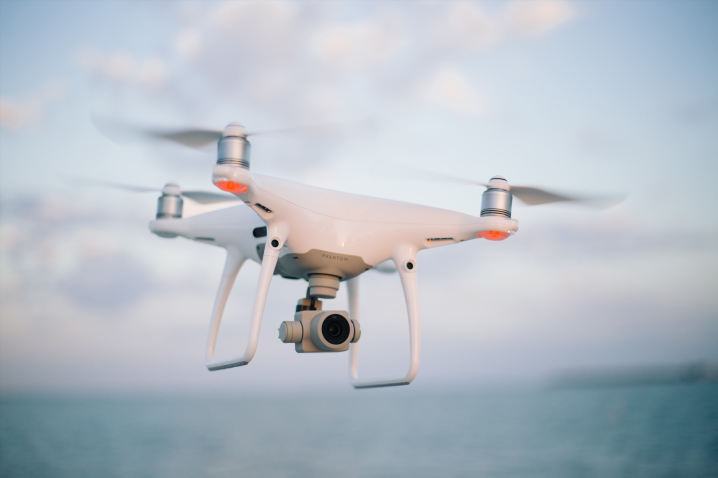
\includegraphics[width=0.75\linewidth]{images/phantom_1} 

}

\caption{Flying drones is fun but can be complicated}\label{fig:drone2}
\end{figure}

\hypertarget{common-UAS-violations}{%
\section{Common UAS Regulation Violations}\label{common-UAS-violations}}

Unless given special permission by the FAA under Part 107 regulations, you are only allowed to operate

\begin{itemize}
\tightlist
\item
  Within Visual Line of Sight
\item
  Not Over People
\end{itemize}

Unfortunately, these are two of the most common UAS violations that we see, especially with videos on the internet. Within the UC system, we are obligated to follow all applicable regulations. So even if you see someone else fly in violation of the laws, it's not ok for you to replicate it.

\hypertarget{visual-line-of-sight}{%
\subsection{Visual Line of Sight}\label{visual-line-of-sight}}

Visual line of sight means that the pilot of the drone must be able to see the drone throughout the entire flight in order to

\begin{itemize}
\tightlist
\item
  know the drone's location
\item
  determine the drone's attitude (orientation), altitude, and direction of flight
\item
  observe the airspace for other air traffic or hazards
\item
  determine that the drone does not endanger the life or property of another
\end{itemize}

The pilot must be \textbf{able} to do the above at all times, but doesn't have to be at all times - meaning he or she may glance at other objects, as long as the drone never leaves the pilot's ability to resume looking at the drone at any time.

At any given time, at least the pilot or any visual observers must maintain visual line of sight - meaning while the pilot is looking away, there must be a visual observer to watch the drone during that time.

\hypertarget{a-speck-in-the-sky-is-not-sufficient}{%
\subsubsection{A Speck in the Sky is not Sufficient}\label{a-speck-in-the-sky-is-not-sufficient}}

At all times, your drone must be close enough that you can tell which direction the drone is facing, how high it is and whether there are any hazards. If all you can see of your drone is a small dot, it means you've gone too far. In practice, your visual distance may be significantly impaired by trees or buildings in the horizon that may make it difficult to see the drone.

Common Drones and recommended max visual distance (on a clear day in a rural location)

\begin{itemize}
\tightlist
\item
  \textbf{DJI Mavic Series} 900 ft horizontal distance
\item
  \textbf{DJI Phantom Series} 1200 ft horizontal distance
\item
  \textbf{DJI Matrice 600 Pro} 3000 ft horizontal distance
\item
  \textbf{Fixed-wing (10ft wingspan)} 5000 ft horizontal distance
\end{itemize}

\hypertarget{you-must-be-able-to-assess-risk}{%
\subsubsection{You must be able to assess risk}\label{you-must-be-able-to-assess-risk}}

If you can't see the sky around the drone or the ground below the drone as in Figure \ref{fig:vlos}, you're not within visual line of sight.

\begin{figure}

{\centering 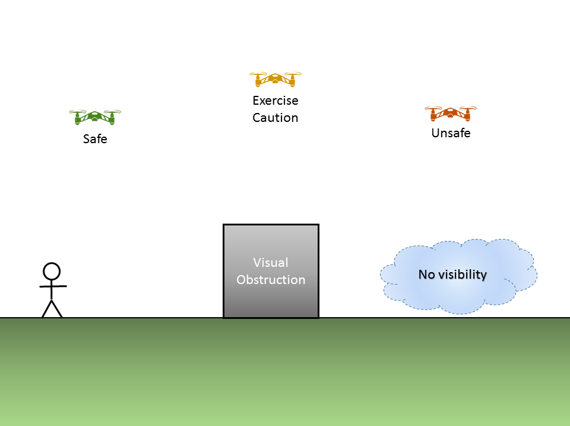
\includegraphics[width=0.8\linewidth]{images/VLOS_G} 

}

\caption{Visual Line of Sight}\label{fig:vlos}
\end{figure}

If this is a scenario that you're looking to do, you may be able to deploy a helper to assist to maintaining a clear flight operational area. However, at no point is the drone allowed to be not viewable by the pilot.

\hypertarget{operations-over-human-beings}{%
\subsection{Operations over Human Beings}\label{operations-over-human-beings}}

Starting April 2021, drones may be issued a special Category certification that allows for operations over people. Table \ref{tab:OOPS} contains an overview of the requirements and restrictions for flight operations over people.

\textbf{Category 0, or Unlisted}

Drones that do not have the Category certification are prohibited from operations over people. In addition to your drone not being allowed to be flown directly over people (107.39), they are prohibited from flying in a manner that poses a hazard to other people in the event of a loss of control of the drone for any reason (107.19(c)). The combination of the two regulations form the majority of the restrictions around people. For drones without the correct Category Certification, you may only fly above people who are part of the immediate flight crew and whose tasks include ensuring flight safety. It is not sufficient to provide spectators with personal protective equipment (PPE), or ask spectators to sign waivers.

\textbf{Category 1}

Category 1 classification is for drones that weigh less than 0.55 lbs and have rotor protection, such as prop guards. These are assumed to have minimal safety risk for operations over people and moving vehicles, and as such, they are allowed to operate in transit over people. This means that the drone can pass over other people, but may not hover over them. If the drone is equipped with Remote ID, then the drone may hover over people, or open air assemblies of people. Starting in September 2023, all drones that do not have Remote ID will be restricted to special zones known as FAA Recognized Identification Areas.

\textbf{Category 2}

Category 2 classification is for drones that have been granted a certificate that they will not cause a severe injury and include rotor protection, such as prop guards. The FAA provides a list of all models of drones that are certified for Category 2 operations. Similarly to Category 1, these are assumed to have safety risk for operations over people and moving vehicles, and as such, they are allowed to operate in transit over people. This means that the drone can pass over other people, but may not hover over them. If the drone is equipped with Remote ID, then the drone may hover over people, or open air assemblies of people. Starting in September 2023, all drones that do not have Remote ID will be restricted to special zones known as FAA Recognized Identification Areas.

\textbf{Category 3}

Category 3 classification is for drones that have been granted a certificate that they will not cause a fatal injury and include rotor protection, such as prop guards. The FAA provides a list of all models of drones that are certified for Category 2 operations. Category 3 is the highest level of allowable risk and are restricted to only in transit flights over people with or without Remote ID. Flying over open air assemblies of people is prohibited unless the drone is equiped with Remote ID and the all persons the drone is flying over has consented.

\textbf{Category 4}

Category 4 classification is a special authorization case for drones that have obtained a Part 21 Airworthiness Certification. The airworthiness certificate will specify the requirements and restrictions for operations over people.

\begin{longtable}[]{@{}
  >{\raggedleft\arraybackslash}p{(\columnwidth - 6\tabcolsep) * \real{0.1795}}
  >{\centering\arraybackslash}p{(\columnwidth - 6\tabcolsep) * \real{0.2308}}
  >{\centering\arraybackslash}p{(\columnwidth - 6\tabcolsep) * \real{0.2308}}
  >{\centering\arraybackslash}p{(\columnwidth - 6\tabcolsep) * \real{0.3590}}@{}}
\caption{\label{tab:OOPS} Operations Over People}\tabularnewline
\toprule
\begin{minipage}[b]{\linewidth}\raggedleft
Category
\end{minipage} & \begin{minipage}[b]{\linewidth}\centering
Requirements
\end{minipage} & \begin{minipage}[b]{\linewidth}\centering
With Remote ID
\end{minipage} & \begin{minipage}[b]{\linewidth}\centering
Without Remote ID
\end{minipage} \\
\midrule
\endfirsthead
\toprule
\begin{minipage}[b]{\linewidth}\raggedleft
Category
\end{minipage} & \begin{minipage}[b]{\linewidth}\centering
Requirements
\end{minipage} & \begin{minipage}[b]{\linewidth}\centering
With Remote ID
\end{minipage} & \begin{minipage}[b]{\linewidth}\centering
Without Remote ID
\end{minipage} \\
\midrule
\endhead
\textbf{Cat 0} & None & Not allowed & Not allowed \\
\textbf{Cat 1} & Under 0.55 lbs Prop Guards & In transit flights over people Flights over open air assemblies & In transit flights over people Only in FRIAs (2023) \\
\textbf{Cat 2} & FAA certification Not cause a severe injury Prop Guards & In transit flights over people Flights over open air assemblies & In transit flights over people Only in FRIAs (2023) \\
\textbf{Cat 3} & FAA certification Not cause a fatal injury Prop Guards & In transit flights over people Flights over consenting open air assemblies & In transit flights over people Only in FRIAs (2023) \\
\textbf{Cat 4} & FAA Airworthiness Certification & In transit flights over people Flights over open air assemblies & In transit flights over people Only in FRIAs (2023) \\
\bottomrule
\end{longtable}

\hypertarget{local-regulations}{%
\section{Local UAS Regulations}\label{local-regulations}}

Any regulatory agency or private property owner can make rules and regulations within their jurisdiction (within reason). The FAA's jurisdiction is the sky and aviation support (licensing, registration, infrastructure).

However, there are other aspects of UAS activity that may be subject to local rules and regulations.

State and local powers include

\begin{itemize}
\tightlist
\item
  Land Use
\item
  Trespass
\item
  Privacy
\item
  Noise ordinances
\item
  Wildlife conservation
\item
  Insurance
\end{itemize}

It is allowed for a State, county or city to place restrictions on where and when drones may take off and land (land use jurisdiction), to define what constitutes invasion of privacy, or to require insurance to operate for or within a jurisdiction. It is your responsibility to

The UC Center of Excellence will help assist you in identifying applicable local regulations, however you are responsible for ensuring your regulatory compliance with all local regulations.

\hypertarget{searching-for-local-uas-regulations}{%
\subsection{Searching for Local UAS Regulations}\label{searching-for-local-uas-regulations}}

There is no easy database for applicable UAS regulations - you will likely have to search multiple locations. Most county and state owned land that is set aside for conservation often have established processes for research permits that are good starting points for UAS use.

Some good resources:

\begin{itemize}
\tightlist
\item
  The \href{https://ucdrones.github.io/map/}{Drone Map of California} lists all of the City and County drone regulations in California
\item
  State level regulations are typically associated with state managed lands, wildlife conservation, privacy and insurance.
\item
  County and Municipal Codes often include regulations for city/county parks and open spaces, typically on land use, trespass and privacy.
\item
  Directors or on-site managers are often good people to ask for permit processes and costs
\end{itemize}

\hypertarget{no-drone-zones}{%
\subsection{No Drone Zones}\label{no-drone-zones}}

Please respect local ordinances, even if you do not agree with them. Do not look for ways to circumvent or utilize a loophole if it is counter to the local communities desires. If you are operating for research or education, you are acting as a representative of the University of California, and we strive to be good neighbors and collaborative with all communities.

\begin{figure}

{\centering 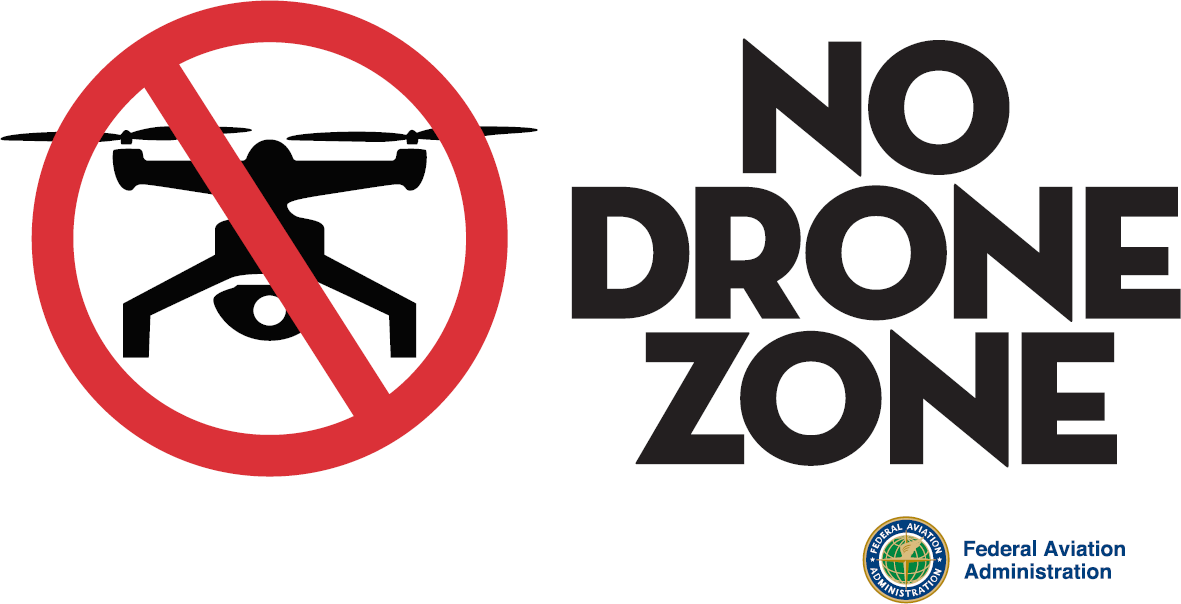
\includegraphics[width=0.8\linewidth]{images/no-drone-zone} 

}

\caption{No Drone Zone Sign}\label{fig:no-drone-zone}
\end{figure}

If you feel strongly, engage the local community in outreach and discussion and work to change their views. But recognize that what you want may not ever be what they want, and you may not be able to change their minds. If you are struggling to get access to your desired site, feel free to reach out to us and we'll see if we can find an alternative location.

\hypertarget{replace-license}{%
\section{Update or Replace a License}\label{replace-license}}

Did you move or change names? Remember that you must inform the FAA within 30 days.

The easiest way to update your information with the FAA is through the Airmen Services page: \url{https://amsrvs.registry.faa.gov/amsrvs/default.asp} (Figure \ref{fig:airmen-services})

On this page, you can

\begin{itemize}
\tightlist
\item
  Change your address
\item
  Order a replacement certificate (\$2)
\item
  Change status of address releasability (by default, all addresses on pilot licenses, including drone licenses are public)
\item
  Remove SSN as certificate number (for those with older manned aviation licenses)
\item
  Request verification of certificate privileges
\end{itemize}

\begin{figure}

{\centering 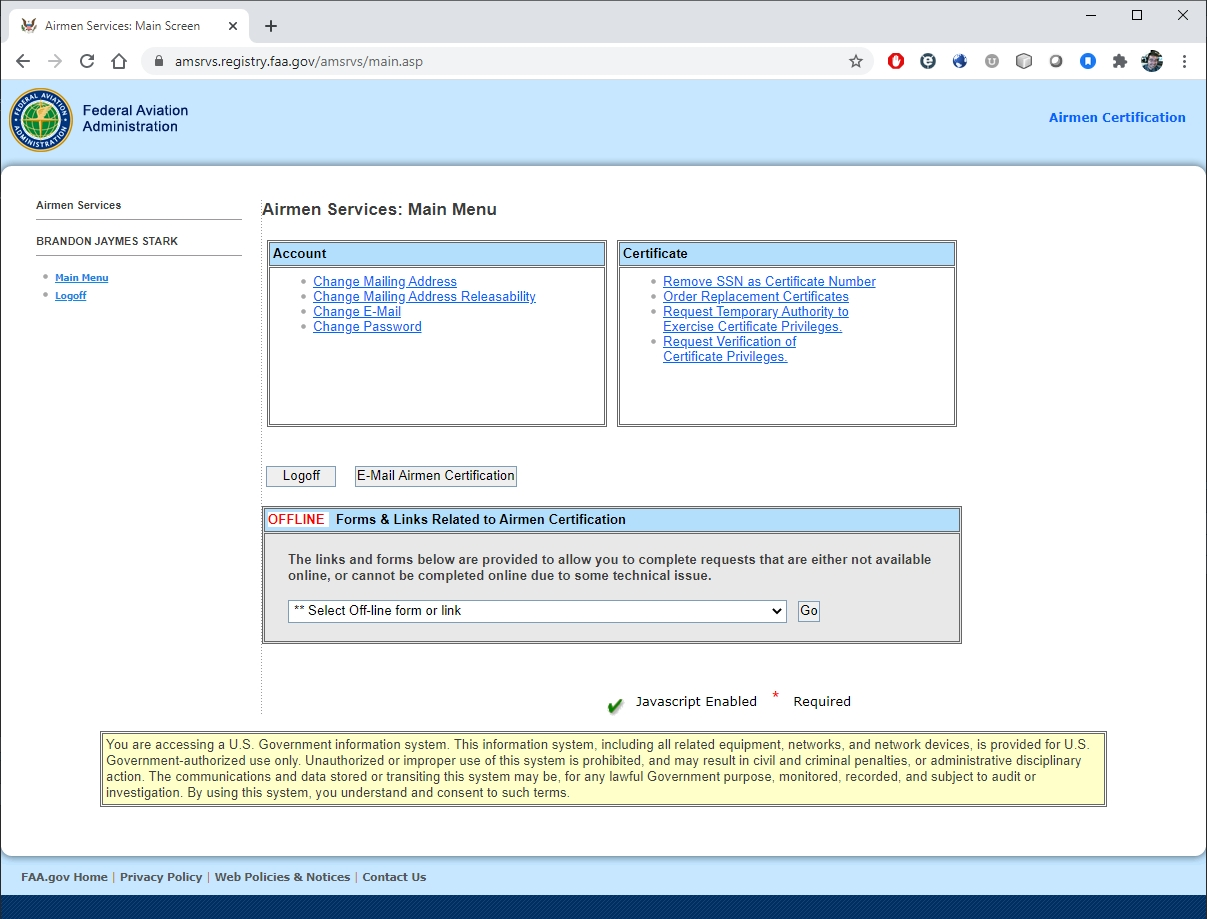
\includegraphics[width=0.7\linewidth]{images/airmen-services} 

}

\caption{FAA Airmen Services Web Page}\label{fig:airmen-services}
\end{figure}

You do not need to order a new Remote Pilot Certificate when you update your address, but ordering a replacement certificate is the only way that you'll get a new copy of your certificate with your new address.

\end{document}
